\documentclass[12pt,a4paper]{report}
\usepackage{changepage}
\usepackage{graphicx}
\usepackage{setspace}
\usepackage[a4paper,
            left=1in,
            right=1in,
            top=1in,
            bottom=1in]{geometry}
            


\let\proof\relax
\let\endproof\relax
\usepackage{amsthm}
\usepackage{amssymb}
\usepackage{thmtools,thm-restate}
\usepackage{xcolor}
\usepackage{tikz}
\usepackage{xspace}

\usepackage{booktabs}   %% For formal tables:
                        %% http://ctan.org/pkg/booktabs
\usepackage{subcaption} %% For complex figures with subfigures/subcaptions
                        %% http://ctan.org/pkg/subcaption


\usepackage{enumitem} 
\usepackage{makecell} 
\usepackage{mathtools}
\usepackage{wrapfig}

\usepackage{amsmath}
\usepackage{pifont}
\usepackage{thm-restate}
\usetikzlibrary{arrows,automata,shapes,decorations,decorations.markings,calc, matrix,decorations.pathmorphing, patterns,backgrounds,shapes.misc,arrows.meta,positioning}

\usepackage{xspace}

\usepackage[ruled,vlined,resetcount,linesnumbered,noend]{algorithm2e}

\usepackage{parskip}

\usepackage{comment}


\usepackage{arydshln}
 \usepackage{multicol}
 \usepackage{multirow}


\usepackage{hyperref}
\usepackage[capitalise]{cleveref}



\usepackage{varwidth}

\usepackage{array}
\newcolumntype{H}{>{\setbox0=\hbox\bgroup}c<{\egroup}@{}}

\usepackage{ifthen}
\usepackage{stackengine}

\usepackage[normalem]{ulem} 

\let\todo\relax
\usepackage{todonotes}
  \newcounter{todocounter}
  \newcommand{\notego}[2][]{\stepcounter{todocounter}\todo[color=red!20, #1]{\thetodocounter: #2}}
  \newcommand{\govind}[1]{{\color{purple}#1}}

\newtheorem{theorem}{Theorem}
\newtheorem{lemma}{Lemma}
\newtheorem{claim}{Claim}
\newtheorem{proposition}{Proposition}
\newtheorem{example}{Example}
\newcommand\xvar{x}
\newcommand\yvar{y}
\newcommand\pb{c}
\newcommand\varset{{\mathbb X}}
\newcommand\regset{{\mathcal R}}
\newcommand\zeroval{0}
\newcommand\valset{{\mathbb V}}
\newcommand\threadset{{\mathcal T}}
\newcommand\procset{{\mathcal T}}
\newcommand\lbl\ell
\newcommand\action\lbl
\newcommand\movesto[1]{\xrightarrow{#1}{}}
\newcommand\lmovesto[1]{\stackrel{#1}\leadsto}
\newcommand\runs{{\it Runs}}
\newcommand\truns{{\it TRuns}}
\newcommand{\setcomp}[2]{\left\{{#1}\mid {#2}\right\}}
\newcommand\succof[1]{{\tt succ}\!\left(#1\right)}
\newcommand\run\rho
\newcommand\thread{S} 
\newcommand\program{\mathsf{Prog}}
\newcommand{\inter}{\rho} 
\newcommand\hh{h}
\newcommand\ii{i}
\newcommand\jj{j}
\newcommand\kk{k}
\newcommand\mm{m}
\newcommand\nn{n}
\newcommand{\init}{\mathsf{init}}
\newcommand{\prem}{\mathsf{P}}
\newcommand{\unn}{\mathsf{U}}
\newcommand{\subb}{\mathsf{Sub}}

\newcommand{\pp}{\pi} 
\newcommand{\vscp}{\textsf{VSC}$^\pp$}
\newcommand{\points}{\mathcal{P}}
\newcommand{\opset}{\Sigma}
\newcommand{\eventset}{\Sigma_{\program}}
\newcommand{\enabled}{\mathsf{Enabled}}
\newcommand{\cgraph}{\mathsf{ConflictGraph}}

\newcommand{\gord}{G^{\mathsf{ord}}}
%% Colors

\colorlet{colorPO}{darkgray!80!black}
\colorlet{colorRF}{blue}
\colorlet{colorOB}{orange}
\colorlet{colorCO}{red!80!black}
\colorlet{colorMO}{red!80!black}
\colorlet{colorFR}{olive}
\colorlet{colorECO}{orange}
\colorlet{colorCOM}{magenta}
\colorlet{colorSW}{teal}
\colorlet{colorHB}{green!40!black}
\colorlet{colorPPO}{magenta}
\colorlet{colorRSEQ}{green!40!black}
\colorlet{colorSC}{violet}
\colorlet{colorHBMO}{brown}
\colorlet{colorPSC}{violet}
\colorlet{colorREL}{olive}
\colorlet{colorWB}{olive}
\colorlet{colorRMW}{brown}
\newcommand\prog{{\mathcal P}}
\newcommand\memmodel{{\mathcal M}}
\newcommand\conf\gamma
\newcommand\terminatedconf{\conf_\downarrow}

\tikzset{
   every path/.style={>=stealth},
   po/.style={->,draw=colorPO,shorten >=-0.5mm,shorten <=-0.5mm},
   ppo/.style={->,draw=colorPPO,shorten >=-0.5mm,shorten <=-0.5mm},
   sw/.style={->,draw=colorSW,shorten >=-0.5mm,shorten <=-0.5mm},
   rf/.style={->,draw=colorRF,dashed,shorten >=-0.5mm,shorten <=-0.5mm},
   mo/.style={->, draw=colorMO,dotted,shorten >=-0.5mm,shorten <=-0.5mm},
    mrf/.style={->,draw=colorRF,dashed,shorten >=-0.5mm,shorten <=-0.5mm},   
   urf/.style={->,draw=colorRF,shorten >=-0.5mm,shorten <=-0.5mm},
   fr/.style={->,draw=colorFR,dashed,shorten >=-0.5mm,shorten <=-0.5mm},
   hb/.style={->,draw=colorHB,thick,shorten >=-0.5mm,shorten <=-0.5mm},
   co/.style={->,draw=colorCO,dotted,very thick,shorten >=-0.5mm,shorten <=-0.5mm},
   rmw/.style={->,draw=colorRMW,thick,shorten >=-0.5mm,shorten <=-0.5mm},
   rseq/.style={->,draw=colorRSEQ,thick,dotted,shorten >=-0.5mm,shorten <=-0.5mm},
   com/.style={->,draw=colorCOM,thick,shorten >=-0.5mm,shorten <=-0.5mm},
}

\newcommand\inarr[1]{\begin{array}{@{}l@{}}#1\end{array}}
\newcommand\inarrC[1]{\begin{array}{@{}c@{}}#1\end{array}}
\newcommand\inpar[1]{\left(\begin{array}{@{}l@{}}#1\end{array}\right)}
\newcommand\inparII[2]{\begin{array}{@{}l@{~~}||@{~~}l@{}}\inarr{#1}&\inarr{#2}\end{array}}
\newcommand\inparIII[3]{\begin{array}{@{}l@{~~}||@{~~}l@{~~}||@{~~}l@{}}\inarr{#1}&\inarr{#2}&\inarr{#3}\end{array}}
\newcommand\inparIV[4]{\begin{array}{@{}l@{~~}||@{~~}l@{~~}||@{~~}l@{~~}||@{~~}l@{}}
\inarr{#1}&\inarr{#2}&\inarr{#3}&\inarr{#4}\end{array}}
\newcommand\inparV[5]{\begin{array}{@{}l@{~~}||@{~~}l@{~~}||@{~~}l@{~~}||@{~~}l@{~~}||@{~~}l@{}}
\inarr{#1}&\inarr{#2}&\inarr{#3}&\inarr{#4}&\inarr{#5}\end{array}}
\newcommand\mytag[1]{\tag{\textsf{#1}}}
\newcommand\inparVI[6]{\begin{array}{@{}l@{~~}||@{~~}l@{~~}||@{~~}l@{~~}||@{~~}l@{~~}||@{~~}l@{~~}||@{~~}l@{}}
\inarr{#1}&\inarr{#2}&\inarr{#3}&\inarr{#4}&\inarr{#5}&\inarr{#6}\end{array}}

%% Math
\newcommand{\set}[1]{\{#1\}}
\newcommand{\setpred}[2]{\{#1 \,|\, #2\}}
\newcommand{\tup}[1]{\langle#1\rangle}
\newcommand{\acyclic}{\mathsf{acyclic}}
\newcommand{\dom}{\mathsf{dom}}
\newcommand{\codom}{\mathsf{codom}}
\newcommand{\imm}{\mathsf{imm}}
\renewcommand{\emptyset}{\varnothing}
\newcommand{\nats}{\mathbb{N}}

%% common events and relations
\newcommand{\R}{\mathsf{R}}
\newcommand{\W}{\mathsf{W}}
\newcommand{\E}{\mathsf{E}}
\newcommand{\F}{\mathsf{F}}
\newcommand{\RMW}{\mathsf{RMW}}
\newcommand{\phase}{\mathsf{phase}}



\newcommand{\RRMW} {\R\cup\RMW}

\newcommand{\WRMW} {\W\cup\RMW}


%% C11

\newcommand{\scmm}{\mathsf{SC}}
\newcommand{\wramm}{\mathsf{WRA}}
\newcommand{\ramm}{\mathsf{RA}}
\newcommand{\rlxmm}{\mathsf{Relaxed}}
\newcommand{\sramm}{\mathsf{SRA}}
\newcommand{\rcmm}{\mathsf{RC20}}
\newcommand{\psmm}{\mathsf{PS}}
\newcommand{\cmmm}{\mathsf{CM}}
\newcommand{\ccmm}{\mathsf{CC}}
\newcommand{\cvmm}{\mathsf{CCv}}
\newcommand{\ctmm}{\mathsf{C11tester}}
\newcommand{\mmorder}{\preccurlyeq}
%

\newcommand{\MOna}{\textsc{na}}
\newcommand{\MOrlx}{\textsc{rlx}}
\newcommand{\MOacq}{\textsc{acq}}
\newcommand{\MOcon}{\textsc{con}}
\newcommand{\MOacqrel}{\textsc{acq-rel}}
\newcommand{\MOacqrlx}{\textsc{acq-rlx}}
\newcommand{\MOrlxrel}{\textsc{rlx-rel}}
\newcommand{\MOrlxrlx}{\textsc{rlx-rlx}}
\newcommand{\MOrel}{\textsc{rel}}
\newcommand{\MOsc}{\textsc{sc}}
\newcommand\oRna   {\mathsf{R}_{\MOna}}
\newcommand\oRrlx  {\mathsf{R}_{\MOrlx}}
\newcommand\oRacq  {\mathsf{R}_{\MOacq}}
\newcommand\oRsc   {\mathsf{R}_{\MOsc}}
\newcommand\oRacqsc {\mathsf{R}_{\sqsupseteq\MOacq}}
\newcommand\oWna  {\mathsf{W}_{\MOna}}
\newcommand\oWrlx  {\mathsf{W}_{\MOrlx}}
\newcommand\oWrel  {\mathsf{W}_{\MOrel}}
\newcommand\oWsc   {\mathsf{W}_{\MOsc}}
\newcommand\oWrelsc {\mathsf{W}_{\sqsupseteq\MOrel}}
\newcommand\Facq{\mathsf{F}_{\MOacq}}
\newcommand\Frel{\mathsf{F}_{\MOrel}}
\newcommand\oCAS{\mathsf{CAS}}
\newcommand{\tuple}[1]{\left\langle#1\right\rangle}
\newcommand{\tuplee}[1]{\left\langle#1\right\rangle}


%% Relations
\newcommand{\po}{\mathsf{\color{colorPO}po}}
\newcommand{\poloc}{\mathsf{\color{colorPO}poloc}}
\newcommand{\rf}{\mathsf{\color{colorRF}rf}}
\newcommand{\rfinv}{\rf^{-1}}
\newcommand{\rv}{\mathsf{\color{colorRF}rv}}
%\newcommand{\co}{\mathsf{\color{colorCO}co}}
\newcommand{\eco}{\mathsf{\color{colorECO}eco}}
\newcommand{\mo}{\mathsf{\color{colorMO}mo}}
\newcommand{\mopartial}{\overline{\mo}}
\newcommand{\frpartial}{\overline{\fr}}
\newcommand{\rfpartial}{\overline{\rf}}
\newcommand{\co}{\mathsf{\color{colorMO}mo}}
\newcommand{\fr}{\mathsf{\color{colorFR}fr}}

\newcommand{\SC}{\mathsf{\color{colorSC}sc}}
\newcommand{\hb}{\mathsf{\color{colorHB}hb}}
\newcommand{\hbloc}{\mathsf{\color{colorHB}hbvar}}
\newcommand{\rfe}{\mathsf{\color{colorRF}rfe}}
\newcommand{\coe}{\mathsf{\color{colorCO}coe}}
\newcommand{\fre}{\mathsf{\color{colorFR}fre}}
\newcommand{\hbmo}{\mathsf{\color{colorHBMO}hbmo}}
\newcommand{\wb}{\mathsf{\color{colorWB}wb}}
\newcommand{\sw}{\mathsf{\color{colorSW}sw}}
\newcommand{\rfi}{\mathsf{\color{colorRF}rfi}}
\newcommand{\coi}{\mathsf{\color{colorCO}coi}}
\newcommand{\fri}{\mathsf{\color{colorFR}fri}}
\newcommand\rloc[1]{{{#1}|_\lloc}}
\newcommand\locx[1]{{{#1}_{x}}}
\newcommand{\ob}[1]{\mathsf{{\color{colorOB}ob}_{#1}}}

%% Program constructs and constants
\newcommand{\bfalse}{\mathsf{false}}
\newcommand{\btrue}{\mathsf{true}}
\newcommand{\Cif}{\mathbf{if}}
\newcommand{\Celse}{\mathbf{else}}
\newcommand{\Cwhile}{\mathbf{while}}
\newcommand{\Cassert}{\mathbf{assert}}
\newcommand{\nw}{\mathbf{new}}
\newcommand{\nul}{\mathbf{NULL}}

\newcommand{\irr}{\mathsf{irr}}
\newcommand{\acy}{\mathsf{acy}}

%% Events and Execution
\newcommand{\op}{\mathsf{op}}
\newcommand{\tid}{\mathsf{tid}}
\newcommand{\event}{e}
\newcommand{\id}{\mathsf{id}}
\newcommand{\llab}{\mathsf{lab}}
\newcommand{\lloc}{\mathsf{var}}
\newcommand{\ord}{\mathsf{ord}}
\newcommand{\val}{\mathsf{val}}
\newcommand{\bottom}{\perp}
\newcommand{\rd}{\mathtt{r}}
\newcommand{\wt}{\mathtt{w}}
\newcommand{\fence}{\mathtt{fence}}
\newcommand{\ud}{\mathtt{rmw}}
\newcommand{\rmw}{\ud}
\newcommand{\fnc}{\mathtt{F}}
\newcommand{\ex}{\mathsf{\color{black}X}}
\newcommand{\partialtext}{\mathsf{partial}}
\newcommand{\expartial}{\overline{\ex}}
\newcommand{\chainid}{\mathsf{chainId}}
\newcommand{\chainhead}{\mathsf{chainHead}}
\newcommand{\ypartial}{\overline{\mathsf{\color{black}Y}}}

%% Complexity
\newcommand{\WComplexity}[1]{\mathcal{W}[#1]}
\newcommand{\NP}{\mathsf{NP}}
\newcommand{\poly}[1]{\text{poly}(#1)}
\newcommand{\NumEvents}{n}
\newcommand{\NumMemory}{d}
\newcommand{\NumThreads}{k}

%% Comments

% PS 

\newcommand\fulfill{\mathsf{fulfill}}

\newcommand{\Path}{\rightsquigarrow}
\newcommand\mapto{\mathsf{mapsTo}}
\newcommand\wtomsg{\mathbb{W}}
\newcommand\rmsg{\mathsf{rmsg}}
\newcommand\wmsg{\mathsf{wmsg}}
\newcommand\ptoe{\mathsf{P2E}}
\newcommand\stepptoe{\mathsf{T}}
\newcommand\stateptoe{\mathbb{S}}
\newcommand\simurel{\mathbb{S}}
\newcommand\gstep{\mathsf{Gstep}}
\newcommand\TS{TS}
\newcommand{\ts}{\mathsf{TS}}
\newcommand\promises{\mathsf{P}}
\newcommand\promise{\mathsf{promise}}
\newcommand\MS{\mathsf{MS}}
\newcommand\TSmap{\mathcal{T\!S}}
\newcommand\M{\mathsf{M}}
\newcommand\TM{\mathsf{TM}}

\newcommand\wmap{\mathbb{W}}

\newcommand\timestamp{\mathsf{ts}}
\newcommand\mbbp{\mathbb{P}}
\newcommand\maxmsg{\mathsf{maxmsg}}



\newcommand\np{\mathsf{NP}}

\newcommand\promisem{\textsc{promise}}

\newcommand\scal{\mathcal{S}}
\newcommand\N{\mathsf{N}}

\newcommand\sstate{\mathsf{state}}

\newcommand\future{\mathsf{future}}
\newcommand\silent{\mathsf{silent}}

\newcommand\allbold[1]{{\boldmath\textbf{#1}}}

\renewcommand{\thefootnote}{\fnsymbol{footnote}}

\newcommand{\MemModel}{\mathcal{M}}
\newcommand{\cg}{\mathsf{CG}}

\newcommand{\celeventester}{\textsf{C11Tester}\xspace}
\newcommand{\Trust}{\textsf{TruSt}\xspace}
\newcommand{\bname}[1]{\textsf{#1}}

% experiments
\newcommand*\circled[1]{\tikz[baseline=(char.base)]{
\node[shape=circle,draw=colorMO,inner sep=2pt] (char) {\tiny{\textcolor{colorMO}{\textbf{#1}}}};}}
\newcommand{\maxspeedup}{$99.3$}
\newcommand{\avgspeedup}{$13.9$}
\newcommand{\expsetone}{\textsf{S1}\xspace}
\newcommand{\expsettwo}{\textsf{S2}\xspace}
\newcommand{\crefrangeconjunction}{-}


\newcommand{\tsomm}{\mathsf{TSO}}
\newcommand{\psomm}{\mathsf{PSO}}
\newcommand{\powermm}{\mathsf{POWER}}





\newcommand{\finegrained}{\mathsf{Fine-grained}}

\newcommand{\Sel}{\mathsf{Sel}}
\newcommand{\Checker}{\mathsf{Checker}}
\newcommand{\BB}{\mathsf{B}}
\newcommand{\Start}{\mathsf{Start}}
\newcommand{\Finish}{\mathsf{Finish}}


\newcommand{\w}{\mathsf{write}}
\newcommand{\re}{\mathsf{read}}
\newcommand{\Ins}{\operatorname{Ins}}
%variable
\newcommand{\var}{\operatorname{var}}
%execution
\newcommand{\Execution}{\mathsf{E}}

%relations and colours

\newcommand{\gw}{\text{GoodW}}


%operations
\newcommand{\plus}{\raisebox{.5\height}{\scalebox{.6}{+}}}

\newcommand{\xra}{\xrightarrow}


\newcommand{\Prog}{\mathsf{Prog}}
\newcommand{\Pp}{\mathcal{P}}
%process
\newcommand{\Proc}{\mathsf{Proc}}
%process name
\newcommand{\process}{\mathsf{P}}
%rf relation set
\newcommand{\relationset}{\mathsf{R}}
\newcommand{\rfFunc}[0]{\mathsf{R_F}}
\newcommand{\Gg}{\mathcal{G}}
\newcommand{\RF}{\mathsf{RF}}
\newcommand{\LW}{\mathsf{LW}}
\newcommand{\TC}{\mathbb{TC}}
\newcommand{\PC}{\mathbb{PC}}
\newcommand{\HB}{\mathbb{HB}}
\newcommand{\THB}{\mathbb{THB}}
\newcommand{\Hh}{\mathbb{H}}
\newcommand{\PO}{\mathsf{PO}}

\newcommand{\LRFH}{\mathbb{LRFH}}
\newcommand{\LRFArr}{\mathsf{LRF}}
\newcommand{\SW}{\mathbb{SW}}
\newcommand{\Uu}{\mathsf{RMW}_{\mathsf{sw}}}
\newcommand{\LWB}{\mathsf{LWB}}
\newcommand{\LRB}{\mathsf{LRB}}
\newcommand{\glw}{\textsf{lastWriteBefore}}
\newcommand{\glwv}{\textsf{lastWriteVBefore}}
\newcommand{\gfwv}{\textsf{firstWriteVAfter}}
\newcommand{\glr}{\textsf{lastReadBefore}}
\newcommand{\glrelw}{\textsf{lastRELWBefore}}
\newcommand{\glrelf}{\textsf{lastRELFBefore}}
\newcommand{\toprfchain}{\textsf{topOfWRfChain}}
\newcommand{\HBMO}{\mathsf{HBMO}}
\newcommand{\PHBMO}{\mathsf{PredHBMO}}
\newcommand{\hbt}{\mathsf{HB}}
\newcommand{\lwbhb}{\mathsf{lastWriteBeforeHB}}
\newcommand{\fwahb}{\mathsf{firstWriteVAfterHB}}

\newcommand{\AcqLst}{\mathsf{CSHist}}
\newcommand{\AccLst}{\mathsf{AccessHist}}
\newcommand{\RdLst}{\mathbb{RList}}
\newcommand{\WtLst}{\mathbb{WList}}

\newcommand{\mx}{\sqcup}
\newcommand{\cle}{\sqsubseteq}
\newcommand{\Cc}{\mathbb{C}}
\newcommand{\CC}{\mathsf{C}}

\newcommand{\Ii}{\mathbb{I}}
\newcommand{\gId}{\mathbbm{g}}
\newcommand{\lastGID}{\gId\mathsf{\_max}}
\newcommand{\lastRelTime}{\mathsf{RelTime\_max}}
\newcommand{\exec}{\mathsf{exec}}
\newcommand{\view}[3]{{#1}_{#2}^{#3}}
\newcommand{\last}{\mathsf{readable}}

\newcommand{\krish}[1]{\textcolor{blue!80!green}{K:#1}}
\newcommand{\sanch}[1]{\textcolor{red!50!black}{SS:#1}}

%%%%%% Macros for algorithms %%%%%%%%
\SetKwProg{myfun}{function}{}{}
\SetKwProg{myhandler}{handler}{}{}
\SetKwFunction{init}{Initialization}
\SetKwFunction{getLW}{getLastWriteBeforeOffline}
\SetKwFunction{poprop}{poPropagate}
\SetKwFunction{joinchangedindex}{pairwiseMaxIndexes}
\SetKwFunction{getLWB}{getLastWriteBefore}
\SetKwFunction{getLRB}{getLastReadBefore}
\SetKwFunction{getLRWB}{getLastReadWriteBefore}
\SetKwFunction{initWtLst}{initWtLst}
\SetKwFunction{initRdLst}{initRdLst}
\SetKwFunction{initWtRdLst}{initWtRdLst}
\SetKwFunction{get}{get}
\SetKwFunction{getHBTS}{getHBTimestamps}
\SetKwFunction{getTCPC}{getTopAndPositionInRFChain}
\SetKwFunction{checkRace}{checkRace}
\SetKwFunction{rdhandler}{readHandler}
\SetKwFunction{wthandler}{writeHandler}
\SetKwFunction{acqhandler}{acquire}
\SetKwFunction{relhandler}{release}
\SetKwInput{Input}{Input}
\SetKwInOut{Output}{Output}
\SetKw{Let}{let}
\SetKw{Break}{break}
\SetKw{NOT}{not}
\SetKw{declare}{declare}
\SetKw{exit}{exit}
\SetKw{Continue}{continue}
\SetKw{Return}{return}
\SetKwFor{Foreach}{for each}{}{}%
\DontPrintSemicolon
\newcommand\mycommfont[1]{\footnotesize\ttfamily\textcolor{blue}{#1}}
\SetCommentSty{mycommfont}
\SetNoFillComment

\def\WCoh{write-coherence}
\def\SWCoh{strong-write-coherence}
\def\RCoh{read-coherence}
\def\WRCoh{weak-read-coherence}
\def\RlxWCoh{relaxed-write-coherence}
\def\RlxRCoh{relaxed-read-coherence}
\def\PORF{porf-acyclicity}
\def\OB{ob-acyclicity}
\def\atomi{atomicity}

\tikzset{
   every path/.style={>=stealth},
   po/.style={->,color=colorPO, thick},
   ppo/.style={->,color=colorPPO, thick},
   sw/.style={->,color=colorSW, thick},
   rf/.style={->,color=colorRF,dashed, thick},
   mrf/.style={->,color=colorRF,dashed, thick},   
   urf/.style={->,color=colorRF, thick},
   fr/.style={->,color=colorFR,dashed, thick},
   hb/.style={->,color=colorHB,thick, thick},
   mo/.style={->,color=colorMO,dotted, very thick},
   dob/.style={->,color=colorDOB, very thick},
   ob/.style={->,color=colorOB, very thick},
   rmw/.style={->,color=colorRMW,thick, thick},
   rseq/.style={->,color=colorRSEQ,thick,dotted, thick},
   com/.style={->,color=colorCOM,thick, thick},
}
\newcommand\initeventset{\E_{\it init}}
\newcommand\initof[1]{\init_{#1}}
\newcommand\initx{\initof\xvar}
\newcommand{\veryshortarrow}[1][3pt]{\mathrel{%
   \hbox{\rule[\dimexpr\fontdimen22\textfont2-.2pt\relax]{#1}{.4pt}}%
   \mkern-4mu\hbox{\usefont{U}{lasy}{m}{n}\symbol{41}}}}


\makeatletter
\newcommand{\labitem}[2]{%
\def\@itemlabel{\textbf{#1}}
\item
\def\@currentlabel{#1}\label{#2}}
\makeatother



\newcommand{\Init}{\mathsf{Init}}
\newcommand{\Fin}{\mathsf{Fin}}



%Single Writer

\SetKwFunction{ChCon}{CheckConsistency}
\SetKwFunction{ChPCon}{CheckPreemptionBoundedConsistency}
\SetKwComment{Comment}{/* }{ */}
\SetKwFunction{Explore}{Explore}
\SetKwFunction{ExploreSC}{ExploreSC}
\SetKwFunction{enable}{EnableEvent}
\SetKwFunction{enableth}{EnableThread}
\SetKwFunction{enablethsc}{EnableThreadSC}
\SetKwFunction{buildgraph}{BuildGraph}
\SetKwProg{Fn}{Function}{:}{}
\newcommand{\pid}[1]{pc_{#1}}
\newcommand{\vu}[2]{Pointer_{#2}^{#1}}
\newcommand{\writer}[1]{\mathsf{Writer}(#1)}
\newcommand{\thr}[1]{#1.thread}
\newcommand{\eventid}[1]{#1.id}
\newcommand{\evar}[1]{#1.var}
\newcommand{\eval}[1]{#1.val}
\newcommand{\AND}{\textbf{and}}
\newcommand{\OR}{\textbf{or}}
\newcommand{\src}[1]{\rf(#1)}
\newcommand{\CheckConsistency}{\textbf{CheckConsistencyRF}}
\newcommand{\rval}[1]{#1.val_{rd}}
\newcommand{\wval}[1]{#1.val_{w}}
\newcommand{\wlast}{\mathsf{Last}}


\newcommand{\threewriter}{\textsc{3-Writer}}
\newcommand{\twowriter}{\textsc{2-Writer}}
\newcommand{\onewriter}{\textsc{1-Writer}}


\newcommand{\update}{\mathsf{Update}}
\newcommand{\Initialize}{\mathsf{Initialize}}
\newcommand{\CheckC}{\mathsf{CheckConsistency}}

 \newcommand*\circl[1]{\tikz[baseline=(char.base)]{
    \node[shape=circle,draw,inner sep=2pt] (char) {#1};}}           
\date{\today}
 
\begin{document}
\makeatletter
\begin{titlepage}


\centering{\Huge\bfseries
Studying Complexity for the Bounded Consistency Testing problem under Weak Memory Models
}

\vspace{1cm}

\begin{center}
A Thesis submitted in partial fulfillment of the requirements for the award of the degree of \bfseries
Doctor of Philosophy in Computer Science 



\vspace{0.3cm}

to

\vspace{0.3cm}

{\Large\bfseries
Chennai Mathematical Institute
}
\vspace{.3cm}


\medskip
\bigskip
%%%%%%%%Author%%%%%%%%
Submitted by

\vspace{0.4cm}

{\Large\bfseries
Sanchari Sil
}



\vspace{1.4cm}

%%%%%%%%%Supervisors%%%%%%%%

Under the supervision of

\vspace{0.4cm}

{\large\bfseries
B. Srivathsan, CMI
\smallskip

and
\medskip

S Krishna, Indian Institute of Technology, Bombay
}


\vfill

\medskip

\Large 
\includegraphics[width=3.5cm]{cmilogo.png}
\medskip

\begin{adjustwidth}{5cm}{5cm}
\centering\small H1 SIPCOT IT Park, Siruseri,  Kelambakkam, \\Tamil Nadu-603103, India
\end{adjustwidth}
\vspace{0.5cm}

{\large\bfseries
\@date
}

\end{center}

\end{titlepage}


\pagenumbering{roman}



\newpage

\chapter*{Declaration}
\addcontentsline{toc}{chapter}{Declaration}



\newpage

\chapter*{Acknowledgements}
\addcontentsline{toc}{chapter}{Acknowledgements}



\newpage

\chapter*{Abstract}
\addcontentsline{toc}{chapter}{Abstract}

 
 
\newpage

\chapter*{List of Publications}
\addcontentsline{toc}{chapter}{List of Publications}



%%%%%%%%%%%%%%%%%%%%%%%%
% TABLE OF CONTENTS
%%%%%%%%%%%%%%%%%%%%%%%%

\tableofcontents

\newpage



%%%%%%%%%%%%%%%%%%%%%%%
% MAIN THESIS
%%%%%%%%%%%%%%%%%%%%%%%

\newpage
\pagenumbering{arabic}

%%%%%%%%%%%%%%%%%%%%%%%%%%%%%%%%%%%%%%%%%%%%%%%%%%
\chapter{Introduction}

 
 
 When a multi-threaded program with a shared memory executes, the order in which memory operations become visible can affect the behavior of the program. The easiest reasoning for such behaviour is to assume that all memory operations occur in a single global order. This assumption is captured by Sequential Consistency (SC)[\cite{SC-Lamport78}]. Under SC, the operations of all processors can be viewed as being interleaved in some sequential order, while the order of operations within each processor is preserved. However, implementing sequential consistency at the hardware level is expensive. Modern processors use several techniques to improve performance, such as store buffers, caches, pipelining, and out-of-order execution. Example, under a memory model called Total Store Order (TSO) \cite{sun1991sparc}, a processor may temporarily keep a store in a buffer while continuing to execute later instructions.  Therfore, the order in which memory operations are observed by different processors may not  always correspond to a single global order. This motivated the development of weak memory models. A weak memory model deviates from SC by setting rules that allow specific memory operations to be observed in an order different from their program order. This encourages hardware optimization while still providing certain guarantees to the programmer.

Several hardware memory models were proposed. Examples include processor consistency (PC) \cite{gharachorloo1990memory}, release consistency (RC) \cite{gharachorloo1990memory}, Weak Ordering \cite{dubois1986memory}, Total Store Order (TSO), Partia Store Order (PSO) \cite{sun1991sparc,sparc1994architecture}.  
Different architecture provided different guarantees. Gharachorloo in 1992  \cite{GHARACHORLOO1992399} summarized the behviours of all these models.

 Besides hardwares, compilers also perform optimizations that can change the order of memory operations thus introducing  additional behaviors that need to be considered. This led to the development of weak memory models extended to programming languages. But weaker model led to more behaviours of the concurrent program. Now it became necessary to check if an observed behaviour is faithful to the permitted model. 
 In 1997, Gibbons and Korach had  studied the problem of testing whether an observed execution of a shared-memory system is consistent with Sequential Consistency. Given the observed reads and writes, their problem asks whether there exists a sequential ordering of these operations that respects the program order of each processor and explains the observed behavior. They showed that this problem is computationally difficult in general, establishing NP-completeness results for several variants. There are several works on testing consistency of SC by varying . \cite{CantinLS05} proved that the problem remains NP-complete even with a single memory
 
 
 
 
location (but with unboundedly many threads), which also implies NP-completness for all memory
models that adhere to the “SC-per-location” property, such as TSO, PSO, RA, SRA and Relaxed 

This led to the development of programming-language memory models, where the language specification itself defines the behavior of concurrent programs. Example include Java Memory Model (JMM), 


. The Java memory model was revised significantly in Java 5, providing a formal description of how threads interact through shared memory. This work highlighted the importance of distinguishing ordinary memory operations from synchronization operations. Similar issues later became central to the design of the C and C++ memory models.


This approach became an important part of the C11 and C++11 memory models. These standards introduced atomic operations with different memory-ordering constraints, including relaxed, acquire, release, acquire-release, and sequentially consistent orderings. Consequently, programmers can select the amount of ordering required for a particular operation instead of having every operation follow sequential consistency.

With the development of formal memory models, the way in which executions are represented has also changed. In earlier discussions, weak memory behavior was often described informally as a processor "reordering" instructions. Modern approaches generally describe an execution using a set of memory events together with relations between those events. For example, program order captures the order of operations within a thread, while a reads-from relation identifies the write from which a read obtains its value. Other relations are used to represent synchronization and ordering constraints. A memory model then specifies which combinations of these events and relations constitute a valid execution.

This formal view is particularly useful for verification. Given an observed execution of a concurrent program, one can ask whether the execution is allowed by a particular memory model. This is the basis of the memory consistency checking problem. Such questions are important because an execution that appears impossible under sequential consistency may nevertheless be valid under a weaker model. Determining whether an observed behavior is consistent with the underlying memory model therefore becomes an important problem in the verification of concurrent programs.

The history of weak memory models can thus be viewed as a gradual movement from a simple global-order view of concurrency towards more flexible and formal descriptions of concurrent executions. Sequential consistency provided a simple starting point, while hardware memory models introduced controlled relaxations to improve performance. Programming-language memory models subsequently had to account for compiler optimizations and synchronization. More recently, formal execution-based models have provided a common framework for studying these behaviors and for developing algorithms to verify them.

Overall, the development of weak memory models reflects a fundamental trade-off between performance and programmability. Stronger memory ordering makes concurrent programs easier to reason about, but it can restrict hardware and compiler optimizations. Weaker ordering provides greater freedom for optimization, but makes reasoning about program behavior more difficult. The study of weak memory models is therefore not only about describing hardware behavior; it is also about finding an appropriate balance between these two requirements.
 

\section{Background and Related Work}

\subsection{Verifying Memory Models}

\section{Contributions}

\section{Organization of the Thesis}

%%%%%%%%%%%%%%%%%%%%%%%%%%%%%%%%%%%%%%%%%%%%%%%%%%
\chapter{Preliminaries}\label{prelim}




This chapter contains all auxiliary definitions to intoduce  the problem of Verifying  Sequential Consistency as appeared in \cite{gibbons}. Particularly it introduces the problem of interest and the relevant theorems for Part A of the thesis. We later shall explore a variant of the VSC problem under weak memory models in Part B. 


\section{Concurrent Programming}

We will fix a finite set $\varset$ of variables (also called memory locations) and a finite value set $\valset$ representing the domain of the variables. There are two kinds of \emph{memory operations}: reading value $d$ on variable $x$, denoted succinctly as $\rd(x, d)$, and writing value $d$ on variable $x$, denoted as $\wt(x, d)$. Let $\opset$ denote the set of memory operations. Since $\varset$ and $\valset$ are finite, $\Sigma$ is finite, and can be seen as a finite alphabet. We make use of standard notations $\Sigma^*$ (resp. $\Sigma^+$) to denote the set of words (resp. non-empty words) from the alphabet $\Sigma$. 

\noindent{\bf{Threads}} A \emph{thread} $\thread$ is a finite (non-empty) sequence of memory operations. In order to distinguish between memory operations appearing in different threads, we equip threads with a unique identifier. Throughout, we assume there are $k$ threads, for some $k \in \nats$, and each thread has an identifier in $\{1, 2, \dots, k\}$. Hence, a thread with identifier $i$ can be seen as a word in $(\{i\} \times \Sigma)^+$. An example of a thread with identifier $2$ would be: 
\begin{align*}
(2: \wt(x, 4)) (2: \rd(y, 3)) (2: \rd(x, 1))
\end{align*}
where $x, y \in \varset$ and $4, 3, 1 \in \valset$. For convenience of exposition, we will call a pair consisting of an identifier and a memory operation as an \emph{event}. Therefore, each thread is a sequence of events with each of them having the same identifier. Since it is a sequence, there is a natural \emph{program order} associated with the events appearing in a thread.

\smallskip 

\noindent{\bf{Concurrent Programs}} A \emph{concurrent program} $\program$ is given by a set of threads $S_1, \dots, S_k$, with $S_i$ having identifier $i$. Let $\eventset$ be the set of all events appearing in $\prog$.  There is a natural \emph{program order} $\po$ induced on $\eventset$: for $e_1, e_2 \in \eventset$, we say $e_1~\po~e_2$ if $e_1, e_2$ belong to the same thread, and $e_1$ immediately precedes $e_2$ in the thread sequence. An \emph{interleaving} $\inter$ of $\program$ is an enumeration of $\eventset$ such that the program order is maintained. A \emph{partial interleaving} is an interleaving of some subset of $\eventset$. Any interleaving is also a partial interleaving.


\smallskip 

\noindent{\bf{Conflicting Pair of Read and Write}} A write $\wt(x,d)$ and a read $\rd(x,d')$ are said to be in conflict when they are on the same variable $x$ 
and $d \neq d'$. 
 
\section{Sequential Consistency}

The model has been first proposed by \cite{SC-Lamport78}. Under  sequentially consistent memory any write or read operations  involving the memory is immediately visible to all the processes of the program. Also, the execution of events in a thread sequence respects the program order ($\po$).
Any partial interleaving $\sigma$ is \emph{sequentially consistent} (SC) if for every $\rd(x, d)$ operation appearing in $\sigma$, there is a preceding $\wt(x, d)$ in $\sigma$ with no other writes conflicting with $\rd(x, d)$ in between. Alternatively, in any interleaving, each read observes the value of the last write (in this interleaving) made to the memory location.  

\paragraph*{Verifying Sequential Consistency} Any memory model is  implemented via hardware or software protocols. As the correctness of concurrent  programs depends on the chosen memory model, a faithful implementation of memory models is essential. 
 Gibbons and Korach~\cite{gibbons} in  \emph{testing shared memories},  presents a way to test whether an observed execution of a multi-threaded program \emph{is consistent with} the (rules of the) underlying memory model. The work by Gibbons and Korach is on SC. 
Let us recall the probem of verifying sequential consistency (VSC) as given in \cite{gibbons}

\begin{center}
  \fbox{%
    \begin{minipage}{0.98\textwidth}
      \noindent \textsc{\textbf{VSC-problem}: Verifying Sequential Consistency} 

      \medskip

     
      \noindent \textbf{Instance:} A concurrent program $\program$. 

      \medskip

      \noindent \textbf{Question:} Is there an interleaving of $\program$ which is sequentially consistent?
    \end{minipage}%
  }
\end{center}

The set of sequences $S_1, \dots, S_k$ forms our observed execution. A ``Yes'' answer to the question above indicates that the observed execution admits an SC behaviour, while a ``No'' answer shows the memory implementation can violate sequential consistency.

Gibbons and Korach~\cite{gibbons} established that the VSC problem is $\NP$-complete. It seems exhaustively exploring all exponentially many possible interleavings is unavoidable. Naturally one might try to find some tractable fragmant of the VSC-problem by bounding other parameters of the program like threads or variables. But the problem still remained hard (see Table 1 of [\cite{gibbons}]).

In Part A of this thesis we have studied the problem by restricting the number of preemtions to be allowed in an interleaving. A preemption occurs when the control switches from one  process to another process without completely executing  the former process. The following definition would make the concept clear. 

\noindent{\bf{Preemptions}} Take a concurrent program $\prog = (S_1, \dots, S_k)$. Let $\sigma = a_1 a_2 \dots a_m$, with each $a_j \in \eventset$, be a partial interleaving of $\prog$. We say that a \emph{preemption} occurs at position $j \in \{1, \dots, m-1\}$ if $a_j$ and $a_{j+1}$ belong to different threads, and $a_j$ is not the last event of its thread. For $\pp \in \nats$, we say that $\sigma$ has $\pp$ preemptions if there are exactly $\pi$ positions in $\sigma$ where preemptions occur. Figure~\ref{fig-onewriter-example} shows some examples.

\begin{figure}[h]
   \def\ystep{0.5}

\centering
	\scalebox{.7}{
\begin{tikzpicture}[yscale=1]
\node (t01) at (-.2, 1.5*\ystep) {$P_1$};
\node (t02) at (1.5, 1.5*\ystep) {$P_2$};
\node (t03) at (3.2, 1.5*\ystep) {$P_3$};



  \node (t11) at (-.2, 0*\ystep) {$1:\wt(x,1)$};
    \node (t12) at (1.5, 0*\ystep) {$2:\rd(x,2)$};
  
    \node (t13) at (3.2, 0*\ystep) {$3:\rd(x,1)$};
    
    \node (t21) at (-.2, -2*\ystep) {$1:\wt(x,2)$};
    \node (t22) at (1.5, -2*\ystep) {$2:\wt(y,1)$}; 
    
  
    
    
    \node (t31) at (-.2, -4*\ystep) {$1:\rd(y,1)$};
   
 
    \draw[po] (t11) -- (t21);
    \draw[po] (t21) -- (t31); 
    
    \draw[po] (t12) -- (t22);
    \end{tikzpicture}}
    
     \caption{The partial interleaving $(1:w(x,1))(3:r(x,1))(1:w(x,2))$ has only one preemption  at $(1:w(x,1))$ while the interleaving $(1:w(x,1))(3:r(x,1))(1:w(x,2)) (2:r(x,2)) (2:w(y,1)) (1:r(y,1))$ has two preemptions at $(1:w(x,1))$ and $(1:w(x,2))$.}\label{fig-onewriter-example}
     
\end{figure}

But why shall we bound preemptions?

Empirical evidence showed that several bugs in multithreaded programs can be caught with very
few preemptions  \cite{QadeerMusuvati}\cite{DBLP:conf/tacas/QadeerR05}   which has resulted in the study of DPOR methods geared
towards finding interleavings with bounded preemptions \cite{vafaedis}.  

With this motivation let us define the following variation of VSC-problem $\pi$.

 

\begin{center}
  \fbox{%
    \begin{minipage}{0.98\textwidth}
      \noindent \textsc{\textbf{VSC$^\pp$-problem}: Verifying Sequential Consistency under $\pp$ preemptions} 

      \medskip

      \noindent \textbf{Fixed:} A constant $\pp \in \mathbb{N}\cup\{0\}$

      \medskip 

      \noindent \textbf{Instance:} A concurrent program $\program$. 

      \medskip

      \noindent \textbf{Question:} Is there an interleaving of $\program$ containing at most $\pp$ preemptions which is sequentially consistent?
    \end{minipage}%
  }
\end{center}

The complexity of the above problem differs with the structure of the program. We have classified the programs into \onewriter~, \twowriter~, and \threewriter~ and studied the corresponding complexity.   

\noindent{\bf{Classification of programs}} In our analysis, we classify programs based on the number of threads that write to a variable. A concurrent program is said to be \onewriter\ if for every variable $x$, there is a single thread with write operations of the form $\wt(x, d)$. Multiple threads can have read operations $\rd(x, d)$ though. Similarly, a concurrent program is said to be \twowriter\ (resp. \threewriter) if there are at most two (resp. three) threads with write operations to each variable. Figures~\ref{fig-onewriter-example} and \ref{fig:example-algo} give examples of \onewriter\ programs.

In later chapters we shall show how the  the complexity of VSC$^\pp$ differs based on whether the program of interest is \onewriter{} or \twowriter{} or \threewriter{} and prove the following theorems. 


First theorem is a tractable result for VSC$^\pp$ when the progam is  \onewriter{}. Note that the VSC-problem for \onewriter{} was $\np$-hard \cite{gibbons}.

\begin{theorem}\label{th:onewriter} \vscp  admits a polynomial-time solution for \onewriter\ programs.  
\end{theorem}

The second theorem states that for multiple writers the VSC$^\pp$ problem becomes $\np$-hard.

\begin{theorem}\label{th:NPhardness}
\vscp is $\NP$-complete, for all $\pi \ge 0$. Hardness holds even for \twowriter\ programs. 
\end{theorem}

The third result gives a conditional lower bound under the Exponential Time Hypothesis (ETH). ETH states that there is no $2^{o(k)} \cdot (k + m)^{\mathcal{O}(1)}$ algorithm for 3-CNF satisfiability, with $k$ being the number of variables and $m$ the number of clauses. 

\begin{theorem} \label{scFinegrained}\label{th:Finegrained}
Under ETH, there is no $2^{o(k)} \cdot n^{\mathcal{O}(1)}$ algorithm for \vscp where $k$ is the number of threads, $n$ is the total number of operations.
\end{theorem}


The proofs of all the above theorem constitute of Part A of this thesis. Part B shall deal with the VSC problem through the lense of weak memory model. These memory models may deviate from stringent SC behaviour and allow re-ordering of memory operations to enhance performance. This would lead to more possible interleavings of a concurrent program as was allowed under $\scmm$.

We particularly care about C-11  memory models in this thesis and shall formally define all the axioms along with the C-11 variant of the problem later in Part B. 


 
\begin{center}
    \chapter*{\centering Part A}
    \addcontentsline{toc}{chapter}{Part A}
\end{center}





%%%%%%%%%%%%%%%%%%%%%%%%%%%%%%%%%%%%%%%%%%%%%%%%%%

\chapter{VSC$^\pp$ Verifying Sequential Consistency under fixed preemptions} \label{sc-1}

The general VSC problem as given in chapter~\ref{prelim} was first studied in \cite{gibbons} to test if shared memory multiprocessors provide a sequentially consistent memory. The problem is in general hard even with restrictions such as bounded threads, bounded variables or just one writer. Later Qadeer and Musuvathi \cite{musuvathi} showed that most  concurrency bugs can manifest within a few number of  preemptions. Also, bounding preemption decreases the state space exploration significantly. So a naural question is what happens to the complexity of the VSC-problem when number of  preemptions is fixed?
We study how the complexity varies across \onewriter{}, \twowriter{} and \threewriter{} programs and discuss the proofs of all the relevant theorems introduced in Chapter~\ref{prelim}.

\section{VSC under fixed preemptions}\label{VSCp}

Recall the VSC$^\pp$-problem from last chapter: given a concurrent program $\program$ and a fixed constant $\pp$, is there an interleaving of $\program$ containing at most $\pp$ preemptions which is sequentially consistent? 

The complexity for VSC$^\pp$ is polynomial for $\onewriter$ programs as given in the next section. The following sections show the hardness results for \twowriter{} and \threewriter{} programs.

\subsection{Results for Single Writer}

We intend to prove the following theorem. 
\begin{theorem}\label{th:onewriter} \vscp  admits a polynomial-time solution for \onewriter\ programs.  
\end{theorem}

For the rest of this section, fix a \onewriter\ program $\program$ with $k$ threads having a total of $n$ events across all threads, 
and a constant $\pp \geq 0$. Here is an overview of our algorithm. 
\begin{description}
\item[Step 1.] Guess a set $\points$ of at most $\pi$ events.
\item[Step 2.] Decide whether there exists an SC interleaving of $\program$ where the preemptions occur exactly after the events in $\points$.
\end{description}
Step 1 can be done in $\mathcal{O}(n^{\pp})$.  For Step 2, we present an algorithm that has complexity $\mathcal{O}(n^3 \cdot k^2 \cdot \pp \cdot \pp!)$.  Hence, the overall complexity  comes to $\mathcal{O}(n^{\pp + 3} \cdot k^2 \cdot \pp \cdot \pp!)$. Since $\pi$ is fixed, we get a polynomial-time algorithm for the \vscp\ problem for \onewriter\ programs. We now present our algorithm with examples.  

 \begin{figure}[t]
 \centering
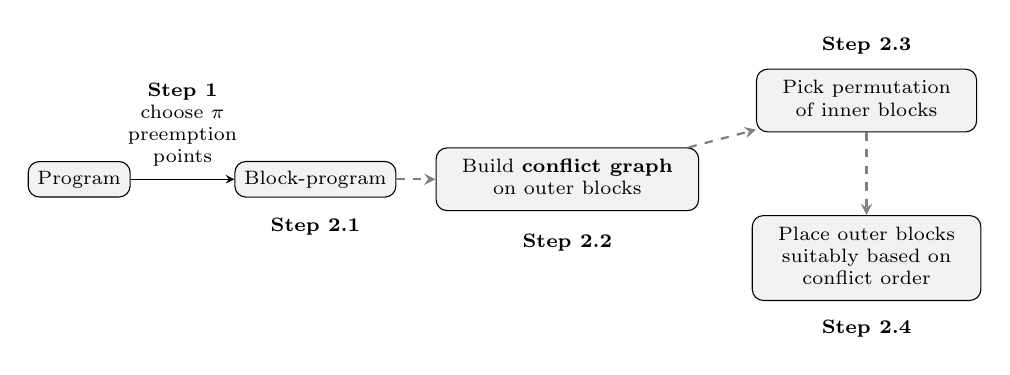
\begin{tikzpicture}[box/.style={rectangle, rounded corners, fill=gray!10, draw}]
  \node [box]  (a) at (0,0) {\scriptsize Program};
  \node [box] (b) at (3,0) {\scriptsize Block-program};
  \node [box] (c) at (6.2,0) {\scriptsize \begin{tabular}{c} Build \textbf{conflict graph} \\ on outer blocks \end{tabular}};
  \node [box] (d) at (10,1) {\scriptsize \begin{tabular}{c} Pick permutation \\ of inner blocks \end{tabular}};
  \node [box] (e) at (10,-1) {\scriptsize \begin{tabular}{c} Place outer blocks \\ suitably based on \\ conflict order \end{tabular}};
 
  

  \begin{scope}[->]
   \draw [>=stealth] (a) to node [above] {\scriptsize \begin{tabular}{c} \textbf{Step 1} \\ choose $\pi$ \\  preemption  \\ points \end{tabular}} (b);
   \draw [thick, dashed, gray] (b) to (c);
   \draw [thick, dashed, gray] (c) to (d);
   \draw [thick, dashed, gray] (d) to (e);
  \end{scope}

  \node at (3, -0.6) {\scriptsize \textbf{Step 2.1}};
  \node at (6.2, -0.8) {\scriptsize \textbf{Step 2.2}};
  \node at (10, 1.7) {\scriptsize \textbf{Step 2.3}};
  \node at (10, -1.9) {\scriptsize \textbf{Step 2.4}};
\end{tikzpicture}
\caption{Schema for the algorithm for \onewriter\ programs}
\label{fig:schema-one-writer}
 \end{figure}

 
The general VSC problem as given in chapter~\ref{prelim} was first studied in \cite{gibbons} to test if shared memory multiprocessors provide a sequentially consistent memory. The problem is in general hard even with restrictions such as bounded threads, bounded variables or just one writer. Later Qadeer and Musuvathi \cite{musuvathi} showed that most  concurrency bugs can manifest within a few number of  preemptions. Also, bounding preemption decreases the state space exploration significantly. So a naural question is what happens to the complexity of the VSC-problem when number of  preemptions is fixed?
We study how the complexity varies across \onewriter{}, \twowriter{} and \threewriter{} programs and discuss the proofs of all the relevant theorems introduced in Chapter~\ref{prelim}.

\section{VSC under fixed preemptions}\label{VSCp}

Recall the VSC$^\pp$-problem from last chapter: given a concurrent program $\program$ and a fixed constant $\pp$, is there an interleaving of $\program$ containing at most $\pp$ preemptions which is sequentially consistent? 

The complexity for VSC$^\pp$ is polynomial for $\onewriter$ programs as given in the next section. The following sections show the hardness results for \twowriter{} and \threewriter{} programs.

\subsection{Results for Single Writer}

We intend to prove the following theorem. 
\begin{theorem}\label{th:onewriter} \vscp  admits a polynomial-time solution for \onewriter\ programs.  
\end{theorem}

For the rest of this section, fix a \onewriter\ program $\program$ with $k$ threads having a total of $n$ events across all threads, 
and a constant $\pp \geq 0$. Here is an overview of our algorithm. 
\begin{description}
\item[Step 1.] Guess a set $\points$ of at most $\pi$ events.
\item[Step 2.] Decide whether there exists an SC interleaving of $\program$ where the preemptions occur exactly after the events in $\points$.
\end{description}
Step 1 can be done in $\mathcal{O}(n^{\pp})$.  For Step 2, we present an algorithm that has complexity $\mathcal{O}(n^3 \cdot k^2 \cdot \pp \cdot \pp!)$.  Hence, the overall complexity  comes to $\mathcal{O}(n^{\pp + 3} \cdot k^2 \cdot \pp \cdot \pp!)$. Since $\pi$ is fixed, we get a polynomial-time algorithm for the \vscp\ problem for \onewriter\ programs. We now present our algorithm with examples.  

 \begin{figure}[t]
 \centering
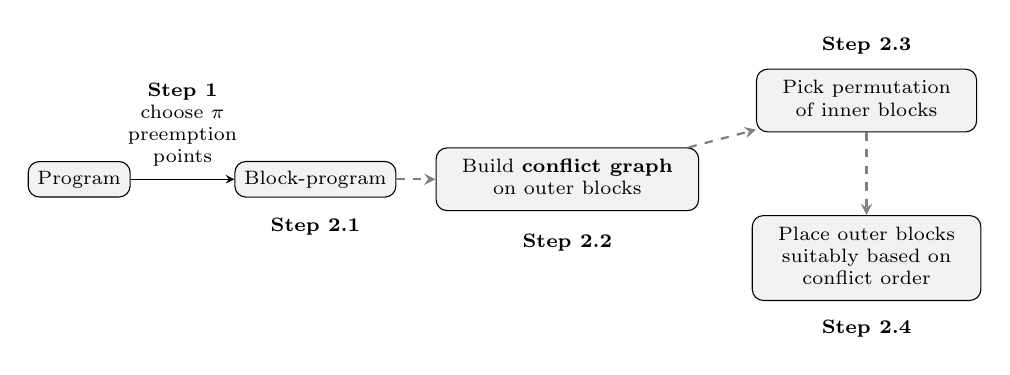
\begin{tikzpicture}[box/.style={rectangle, rounded corners, fill=gray!10, draw}]
  \node [box]  (a) at (0,0) {\scriptsize Program};
  \node [box] (b) at (3,0) {\scriptsize Block-program};
  \node [box] (c) at (6.2,0) {\scriptsize \begin{tabular}{c} Build \textbf{conflict graph} \\ on outer blocks \end{tabular}};
  \node [box] (d) at (10,1) {\scriptsize \begin{tabular}{c} Pick permutation \\ of inner blocks \end{tabular}};
  \node [box] (e) at (10,-1) {\scriptsize \begin{tabular}{c} Place outer blocks \\ suitably based on \\ conflict order \end{tabular}};
 
  

  \begin{scope}[->]
   \draw [>=stealth] (a) to node [above] {\scriptsize \begin{tabular}{c} \textbf{Step 1} \\ choose $\pi$ \\  preemption  \\ points \end{tabular}} (b);
   \draw [thick, dashed, gray] (b) to (c);
   \draw [thick, dashed, gray] (c) to (d);
   \draw [thick, dashed, gray] (d) to (e);
  \end{scope}

  \node at (3, -0.6) {\scriptsize \textbf{Step 2.1}};
  \node at (6.2, -0.8) {\scriptsize \textbf{Step 2.2}};
  \node at (10, 1.7) {\scriptsize \textbf{Step 2.3}};
  \node at (10, -1.9) {\scriptsize \textbf{Step 2.4}};
\end{tikzpicture}
\caption{Schema for the algorithm for \onewriter\ programs}
\label{fig:schema-one-writer}
 \end{figure}

\subsubsection*{Step 2.1. Partition the program $\program$ into Blocks : Block Programs}

A subset of events $\points \subseteq \eventset$ represents \emph{preemption points} if no event in $\points$ is the last event of its thread. Assume we have chosen a specific set $\points$ of preemption points. Note that when $\pi=0$, $\points$ is the emptyset.


Let $c^\points_i \ge 0$ be the number of events of thread $i$ in $\points$. 
We will omit the superscript and simply write $c_i$ when $\points$ is clear from the context. Furthermore,  $\sum_{i} c_i \le \pp$. Each thread $S_i$ can then be divided into blocks, based on the events of $S_i$ that are in $\points$, as explained next.


Consider thread $S_i$ as 

 $S_i = a_1 a_2 \dots a_m$.

Assume we guess events $a_{j_1}, a_{j_2}, a_{j_3}$ with $1 \le j_1 < j_2 < j_3 < m$ to be the events after which preemptions occur (in general, we guess $c_i$ events in thread $S_i$; we have taken $c_i = 3$ just as an example). This divides the thread into four blocks:
\begin{align*}
b^i_1: a_1 \dots a_{j_1} \qquad b^i_2: a_{j_1 + 1} \cdots a_{j_2} \qquad b^i_3: a_{j_2 + 1} \cdots a_{j_3} \qquad b^i_4: a_{j_3 + 1} \cdots a_m
\end{align*}
Each block is a contiguous set of events of a thread, and in every interleaving where the preemption points for $S$ occur at $a_{j_1}, a_{j_2}, a_{j_3}$, the events within a block appear contiguously, and moreover no two consecutive blocks of a thread appear next to each other. 

We denote the thread $S_i$ partitioned into blocks as $S_i^\points$. 
\begin{align*}
    \thread^\points_i = b^i_1 \cdot b^i_2 \cdots b^i_{c_i + 1}
\end{align*}
where each block $b^i_j$ is a contiguous sequence of events of $\thread_i$ ending in a preeemption point, as explained above. We call $\thread^\points_i$ as a \emph{block-thread}, and the set of block-threads $\thread^\points_1, \thread^\points_2, \dots, \thread^\points_k$ a \emph{block-program}, which we denote by $\program^\points$.

\begin{example}\label{eg:block-program}
In Figure~\ref{fig-onewriter-example} if $\points_1=\{(1:w(x,1)), (2:r(x,2))\}$ be the preemption points, then the block-program w.r.t. $\points_1$ would look as follows: 
\begin{alignat*}{2}
    \thread^{\points_1}_1 &=b^1_1\cdot b_2^1 &&=(1:w(x,1)) ~\cdot~ (1:w(x,2))(1:r(y,1))\\
     \thread^{\points_1}_2 
     &= b^2_1\cdot b_2^2 &&=(2:r(x,2)) ~\cdot~ (2:w(y,1))\\
      \thread^{\points_1}_3 &=b^3_1 &&=(3:r(x,1))
\end{alignat*}
where the first thread $\thread^{\points_1}_1$ is partitioned as  $b_1^1=(1:w(x,1))$, $b_2^1=(1:w(x,2))(1:r(y,1))$, and similarly for the other threads. 

Likewise, for the set $\points_2=\{(1:w(x,1)), (1:w(x,2))\}$ of preemption points, the block-program w.r.t. $\points_2$ would look as follows: 
\begin{alignat*}{2}\label{blockpartition}
    \thread^{\points_2}_1 &= b^1_1\cdot b_2^1\cdot b_3^1 &&=(1:w(x,1)) ~\cdot~(1:w(x,2))~\cdot~ (1:r(y,1))\\
     \thread^{\points_2}_2 
     &=b_1^2 &&=(2:r(x,2))(2:(w(y,1)))\\
      \thread^{\points_2}_3 &=b_1^3 &&= (3:r(x,1))
\end{alignat*}
Finally, for the set $\points_3=\emptyset$, $\thread^{\points_3}_1{=} b^1_1 {=} \thread_1$,  
$\thread^{\points_3}_2{=} b^2_1 {=} \thread_2$ and $\thread^{\points_3}_3{=} b^3_1 {=} \thread_3$ consist of a single block each.
\end{example}

A better illustration is given in right side of Figure~\ref{fig:example-algo} 
\subsubsection*{Sequential Consistency for Block Programs} We extrapolate the notion of sequential consistency in a natural way to the obtained block-program. A partial interleaving $\sigma^\points$ of $\program^\points$ is sequentially consistent if the partial interleaving $\sigma$ of the original program $\program$ obtained by expanding each block of $\sigma^\points$ into the contiguous sequence of events that it represents, is sequentially consistent. 

\begin{example}\label{eg:sc-for-block-programs}
Consider the program in Figure~\ref{fig-onewriter-example}. Let us call it $\program$. Then if we choose the set of preemption points $\points_1$ as in Example~\ref{eg:block-program}, $\sigma^{\points_1}=b^1_1\cdot b^3_1 \cdot b_1^2\cdot b_2^1\cdot b_2^2 $ is an interleaving for the block-program $\program^{\points_1}$. Note that this is not sequentially consistent as the last write on $x$ before $\rd(x,2)$ in $\sigma^{\points_1}$ is $\wt(x,1)$, which conflicts with $\rd(x,2)$. 
 Hence $\rd(x,2)$ has no write to read from.  
An example of a sequentially consistent interleaving of blocks from $\program^{\points_2}$ is: $\sigma^{\points_2}=b_1^1\cdot b_1^3\cdot b_2^1\cdot b_1^2\cdot b_3^1$.
\end{example}


\begin{figure}[t]
 \centering
 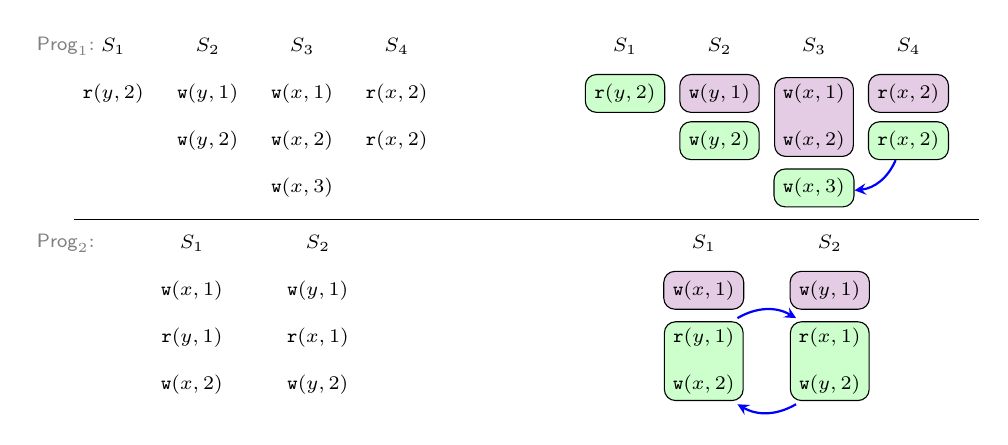
\begin{tikzpicture}
\begin{scope}
 \node at (0,0) {\scriptsize $S_1$};
 \node at (0,-0.6) {\scriptsize $\rd(y,2)$};
 \node at (1.2, 0) {\scriptsize $S_2$};
 \node at (1.2, -0.6) {\scriptsize $\wt(y,1)$};
 \node at (1.2, -1.2) {\scriptsize $\wt(y,2)$};
 \node at (2.4, 0) {\scriptsize $S_3$};
 \node at (2.4, -0.6) {\scriptsize $\wt(x,1)$};
 \node at (2.4, -1.2) {\scriptsize $\wt(x,2)$};
 \node at (2.4, -1.8) {\scriptsize $\wt(x,3)$};
 \node at (3.6, 0) {\scriptsize $S_4$};
 \node at (3.6, -0.6) {\scriptsize $\rd(x, 2)$};
 \node at (3.6, -1.2) {\scriptsize $\rd(x, 2)$};
\end{scope}

\begin{scope}[xshift=6.5cm, outer/.style={rectangle, rounded corners, fill=green!20, draw}, inner/.style={rectangle, rounded corners, fill=violet!20, draw}]
\node at (0,0) {\scriptsize $S_1$};
 \node [outer] at (0,-0.6) {\scriptsize $\rd(y,2)$};
 \node at (1.2, 0) {\scriptsize $S_2$};
 \node [inner] at (1.2, -0.6) {\scriptsize $\wt(y,1)$};
 \node [outer] at (1.2, -1.2) {\scriptsize $\wt(y,2)$};
 \node at (2.4, 0) {\scriptsize $S_3$};
 \draw [rounded corners, fill=violet!20] (1.9, -0.4) rectangle (2.9, -1.4);
 \node  at (2.4, -0.6) {\scriptsize $\wt(x,1)$};
 \node  at (2.4, -1.2) {\scriptsize $\wt(x,2)$};
 \node [outer] (b) at (2.4, -1.8) {\scriptsize $\wt(x,3)$};
 \node at (3.6, 0) {\scriptsize $S_4$};
 \node [inner] at (3.6, -0.6) {\scriptsize $\rd(x, 2)$};
 \node [outer] (a) at (3.6, -1.2) {\scriptsize $\rd(x, 2)$};
\end{scope}

\draw [->, thick, blue] (a) to [bend left] (b);

\draw (-0.5,-2.2) -- (11,-2.2);

%\node at (1.8, -2.2) {\scriptsize $\program_1$};
\node [left, thick, gray] at (-0.1, 0) {\scriptsize $\program_1$:};
\node [left, thick, gray] at (-0.1, -2.5) {\scriptsize $\program_2$:};

\begin{scope}[yshift=-2.5cm]
\node at (1, 0) {\scriptsize $S_1$};
\node at (1, -0.6) {\scriptsize $\wt(x,1)$};
\node at (1, -1.2) {\scriptsize $\rd(y,1)$};
\node at (1, -1.8) {\scriptsize $\wt(x,2)$};

\node at (2.6, 0) {\scriptsize $S_2$};
\node at (2.6, -0.6) {\scriptsize $\wt(y,1)$};
\node at (2.6, -1.2) {\scriptsize $\rd(x,1)$};
\node at (2.6, -1.8) {\scriptsize $\wt(y,2)$};

%\node at (1.8, -2.2) {\scriptsize $\program_2$};
\end{scope}

\begin{scope}[xshift = 6.5cm, yshift=-2.5cm, outer/.style={rectangle, rounded corners, fill=green!20, draw}, inner/.style={rectangle, rounded corners, fill=violet!20, draw}]
\node at (1, 0) {\scriptsize $S_1$};
\node [inner] at (1, -0.6) {\scriptsize $\wt(x,1)$};
\draw [rounded corners, fill = green!20] (0.5, -1) rectangle (1.5, -2);
\node (c) at (1, -1.2) {\scriptsize $\rd(y,1)$};
\node (e) at (1, -1.8) {\scriptsize $\wt(x,2)$};

\node at (2.6, 0) {\scriptsize $S_2$};
\node [inner] at (2.6, -0.6) {\scriptsize $\wt(y,1)$};
\draw [rounded corners, fill = green!20] (2.1, -1) rectangle (3.1, -2);
\node (d) at (2.6, -1.2) {\scriptsize $\rd(x,1)$};
\node (f) at (2.6, -1.8) {\scriptsize $\wt(y,2)$};

\draw [thick, blue, ->] (c) to [bend left] (d);
\draw [thick, blue, ->] (f) to [bend left] (e);
\end{scope}

\end{tikzpicture}
\caption{Programs $\program_1$ and $\program_2$ on the left, their corresponding block-programs on the right w.r.t. chosen preemption points. Inner blocks are coloured in violet, and outer blocks in green. The blue edges denote edges in the conflict graph of the outer nodes.}
\label{fig:example-algo}
\end{figure}

\begin{figure}[t]
\centering
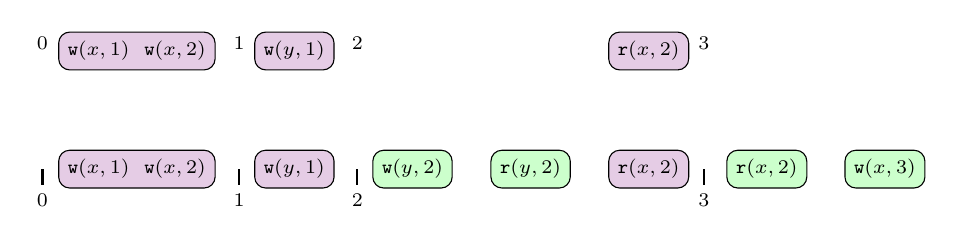
\begin{tikzpicture}[outer/.style={rectangle, rounded corners, fill=green!20, draw}, inner/.style={rectangle, rounded corners, fill=violet!20, draw}]

 \node [inner] (a1) at (0,1.5) {\scriptsize $\wt(x,1)~~\wt(x,2)$};
 % \draw [thick] (-1.2, 2) -- (-1.2, -0.2);
  \node at (-1.2, 1.6) {\scriptsize $0$};
  %\node at (0,-0.6) {\scriptsize $\wt(x,2)$};
  
  
  \node [inner] (b1) at (2,1.5) {\scriptsize $\wt(y,1)$};
%\draw [thick] (1.3, 0) -- (1.3, -0.2);
  \node at (1.3, 1.6) {\scriptsize $1$};

 % \draw [thick] (2.8, 0) -- (2.8, -0.2);
  \node at (2.8, 1.6) {\scriptsize $2$};

  \node [inner] (c1) at (6.5,1.5) {\scriptsize $\rd(x, 2)$};
  %\draw [thick] (7.2, 0) -- (7.2, -0.2);
  \node at (7.2, 1.6) {\scriptsize $3$};

  %\node [outer] at (3.5, 0) {\scriptsize $\wt(y, 2)$};
  %\node [outer] at (5, 0) {\scriptsize $\rd(y, 2)$};
  %\node [outer] at (8, 0) {\scriptsize $\rd(x,2)$};
  %\node [outer] at (9.5, 0) {\scriptsize $\wt(x,3)$};


  %\node [rectangle, rounded corners, fill=red!20, minimum size=1cm, draw] (a) at (0,-0.3) {};
  \node [inner] (a) at (0,0) {\scriptsize $\wt(x,1)~~\wt(x,2)$};
  \draw [thick] (-1.2, 0) -- (-1.2, -0.2);
  \node at (-1.2, -0.4) {\scriptsize $0$};
  %\node at (0,-0.6) {\scriptsize $\wt(x,2)$};
  
  
  \node [inner] (b) at (2,0) {\scriptsize $\wt(y,1)$};
\draw [thick] (1.3, 0) -- (1.3, -0.2);
  \node at (1.3, -0.4) {\scriptsize $1$};

  \draw [thick] (2.8, 0) -- (2.8, -0.2);
  \node at (2.8, -0.4) {\scriptsize $2$};

  \node [inner] (c) at (6.5,0) {\scriptsize $\rd(x, 2)$};
  \draw [thick] (7.2, 0) -- (7.2, -0.2);
  \node at (7.2, -0.4) {\scriptsize $3$};

  \node [outer] at (3.5, 0) {\scriptsize $\wt(y, 2)$};
  \node [outer] at (5, 0) {\scriptsize $\rd(y, 2)$};
  \node [outer] at (8, 0) {\scriptsize $\rd(x,2)$};
  \node [outer] at (9.5, 0) {\scriptsize $\wt(x,3)$};

  
\end{tikzpicture}
\caption{A permutation of inner blocks (above), and an interleaving obtained by 
inserting outer blocks at appropriate positions (below).}
\label{fig:example-algo-final-step}
\end{figure}


Thus,  there is a direct correspondence between interleavings of $\program$ and interleavings of a block-program $\program^\points$. When consecutive blocks within a thread do not appear together in an interleaving, then, it represents an interleaving of $\program$ where the preemptions occur exactly at $\points$.  We state this observation in the following lemma, whose proof follows directly from the definition of block-programs.


\begin{lemma}
Let $\points$ be a set of preemption points of $\program$. Then, $\program$ has a sequentially consistent interleaving where the preemptions occur at $\points$, iff the block-program $\program^{\points}$ has a sequentially consistent interleaving where no two consecutive blocks come from the same thread. 
\end{lemma}

The question therefore boils down to checking whether there is a sequentially consistent interleaving of $\program^{\points}$.

\noindent{\bf{Finding a sequentially consistent interleaving of a block-program}}.  
Recall that each thread has been divided into $c_i + 1$ blocks. A naive solution would be to enumerate all possible orderings of the $\sum_i (c_i + 1)$ blocks satisfying the program order and verify sequential consistency of each of them. However:
\begin{equation} 
  \sum_i (c_i + 1) = \sum_i c_i + \sum_i 1 \le \pp + k  \label{eq:naive} 
\end{equation} 
This only gives a complexity bounded by $(\pp + k)!$ which is not polynomial-time  when $\pp$ is the only fixed parameter.
Therefore, we propose a different procedure. 

\paragraph*{Dividing the block program into inner blocks and outer blocks.} Suppose $\program^{\points}$ is a block-program defined on the set of preemption points $\points$. We call the last block of any thread in $\program^{\points}$ as outer block and all other non-last blocks as inner blocks. In Figure~\ref{fig:example-algo}, all the violet blocks are inner blocks while the green blocks are outer blocks. As each inner block ends with a preemption point in $\points$, there are total $\pp$ inner blocks. Then the total number of outer blocks is $k$. We then  do a pre-processing that would add some ordering among the outer blocks of $\program^{\points}$ and discard the chosen set of preemptions $\points$ immediately if a cycle is found. 



\subsubsection*{Step 2.2. Conflict graph analysis on outer blocks}

By the end of Step 2.2, we have now identified the inner blocks and the outer blocks of $\program^{\points}$. 

We say the block $b_w$ conflicts block $b_r$ if (1) they belong to different threads, (2) there is a variable $x$ such that last write on $x$ in $b_w$ is in conflict with some read on $x$ in $b_r$. Then we order them as $b_r \to b_w$. Now look at the set of all outer blocks of $\program^{\points}$. For each outer block $b_w$, find if it is in conflict with some other outer block $b_r$. If yes, put the the order of conflict $b_r \to b_w$. This says that in any interleaving, $b_r$ appears before $b_w$. As $b_w$ is the last block of its thread, if $b_w$ writes to $x$ and is in conflict with $b_r$, $b_w$ cannot be executed before $b_r$. The blue edges in Figure~\ref{fig:example-algo} represents conflict order among the outer blocks. 

We can construct a conflict graph $G^{\program
^{\points}}$ as follows: For each outer block there is a node in $G$. For each outer block $b_w$ if it conflicts some other outer block $b_r$, we put the edge $b_r \to b_w$. In Figure~\ref{fig:example-algo},  for $\program_1$, $\rd(x, 2)$ should appear before $\wt(x, 3)$; for $\program_2$, there are two induced orderings due to the different variables $x$ and $y$.

If there is a cycle in the conflict graph (as in $\program_2$) we declare that there exists no SC interleaving for the chosen set of preemptions $\points$. If there is no such cycle (for instance, $\program_1$), we move to Step 2.3. 

\paragraph*{Complexity}: For each of the $k$ outer blocks we check if it conflicts some other outer block. To do this, given an outer block $b$, for every variable $x$ that the block writes, we check if the last write on $x$ in $b$ is in conflict with any read of other outer blocks. Thus constructing the graph takes $\mathcal{O}(n\cdot k)$ time. Next we check for a cycle. This takes not more than $\mathcal{O}(k^2)$ time. As $k< n$, Step 2.2 would take $\mathcal{O}(n\cdot k)$ time to run. 

\subsubsection*{Step 2.3. Placing outer blocks in a Permutation of Inner Blocks.}

Consider all possible permutations of the inner blocks. Since there are at most $\pp$ in number, there are at most $\pp!$ permutations. The goal is to check if we can place the $k$ outer blocks between these inner blocks so as to obtain an SC interleaving. In Figure~\ref{fig:example-algo-final-step}, the top illustrates an ordering for inner blocks.  We have also marked the positions around the inner blocks (in the figure, they are marked as $0, 1, 2$ and $3$). The outer blocks need to be placed appropriately.

\subsubsection*{Step 2.4. Placing the outer blocks respecting conflict}

After the conflict analysis returns no cycle for the conflict graph $G^{\program
^{\points}}$, in Step 2.3 we choose a permutation $p$ of the inner blocks. On each of these $\pp!$ permutations we now call Algorithm~\ref{pseudocode:vscp-interleaving}. This is the final step which returns an SC interleaving of the blocks of $\program^{\points}$. For this section $\program$ refers to $\program^{\points}$ and $G$ refers to $G{\program
^{\points}}$. We omit the superscript of the notations.



\begin{algorithm}[h]
\caption{Module to obtain an $\scmm$-consistent block interleaving from a given block program $\program$}\label{pseudocode:vscp-interleaving}

\Input{A block-program $\program$ of a $\onewriter$ program, a permutation $\sigma=\{b_1,b_2,\cdots,b_{\pp}\}$  on inner blocks and an acyclic conflict graph $G$ on the outer blocks}
\Output{an $\scmm$ consistent interleaving of blocks}
\smallskip

\Fn{CheckSC($\program$, $\sigma$, $G$)}{

    $G'=$ a linearization of $G$;
    
    $test=0$;
    
    $b'=\epsilon$;
    
    Add dummy block $b_{\pp+1}$ to $\sigma$;
    
    \For{$i\gets0$ \KwTo $\pp+1$}{\label{for-loop-outer}
        
        \While{there exists an outer block which is enabled}{\label{While-loop}
        
        Choose the earliest enabled block $b$ in $G'$;
        
        \For{$j\gets i+1$ \KwTo $\pp$}{\label{For-loop-iner}
                \If{$b$ conflicts $b_j$} {\label{if-conflict}
                
                test$=1$; 
                
                \Break;}
            
            }
            
            \If{$test=0$}{
            
            Place $b$ between $b'$ and $b_{i+1}$ in $\sigma$;
            
            $b'=b$;
            
            Remove $b$ from $G'$;}
        
        }
        
        $b'=b_{i+1}$;
        

    }
    
    \If{$\sigma$ is $\scmm$-consistent and $G'$ is empty}{\Return 1;}
}


\end{algorithm}

Algorithm~\ref{pseudocode:vscp-interleaving} describes Step 2.4 of the polynomial time algorithm for \vscp. The input is a block-program of a single writer system  divided into inner and outer blocks, a permutation of the inner blocks $\sigma$ and a conflict graph $G$ on the outer blocks. Recall that outer blocks are the last blocks of each block sequence. It takes a linearization $G'$ of $G$ and uses it to place the outer blocks in their correct position in $\sigma$ so that the resulting interleaving is $\scmm$-consistent. 

Description: The algorithm~\ref{pseudocode:vscp-interleaving} chooses a linearization $G'$ of $G$. For each position between the consecutive inner block in $\sigma$, beginning from the left to $b_1$, the algorithm places all enabled outer blocks such that the conflict order of $G$ is satisfied. Note that any outer  block $b$ is enabled at some position only if (1) all blocks above it in its thread are already in sigma before the currently considered position (2) if the last block before the current position is $b'$ and the prefix of $\sigma$ upto $b'$ is $\sigma'$, then $\sigma'\cdot b$ should be $\scmm$-consistent. The variable $b'$ captures the last position in $\sigma$ where a block has been inserted. Moreover, $b$ should not conflict any inner block of $\sigma$ at any later position. This is captured by the condition of the \emph{If} statement in line~\ref{if-conflict}. At the end of the outer for-loop, if no more outer blocks remain to be inserted in $\sigma$, and the resulting interleaving $\sigma$ is $\scmm$-consistent, return 1.

Continuing with our running example $\program_1$ in Figure~\ref{fig:example-algo-final-step}, at position $0$, none of the outer blocks is enabled: the outer block in $S_1$ requires a writing source, and the outer blocks in the other threads cannot be scheduled unless earlier blocks in the program order are completed. So we move to position $1$. At position $1$, the outer block $\wt(x, 3)$ of $S_3$ is enabled since the inner block $\wt(x,1).\wt(x,2)$ of $S_3$ 
appears already.  However, we cannot place it at position 1 for two reasons: firstly, it conflicts the inner block $\rd(x, 2)$ that appears in front of position 3 to the right; and secondly there is an outer $\rd(x,2)$ block which needs to appear before $\wt(x, 3)$ according to the ordering induced by the conflict. Therefore, we do not place it at position $1$ and move on to position $2$. At position $2$, the enabled outer blocks are $\wt(y, 2)$ and $\wt(x, 3)$. We place $\wt(y, 2)$ and not $\wt(x, 3)$ for the same reasons as above. Once $\wt(y, 2)$ is placed, the outer block $\rd(y, 2)$ is also enabled. We place it and move on to position $3$. Here, both $\wt(x, 3)$ and the outer block $\rd(x, 2)$ are enabled. Based on the conflict ordering, we place $\rd(x, 2)$ followed by $\wt(x, 3)$. 

Thus, at each position in a given permutation of inner blocks,
 we find the enabled outer blocks among the ones yet to be scheduled, and  place them according to the ordering induced by the conflicts. Moreover, we place an outer block at a position only if it does not conflict any inner block appearing later. Placing an outer block at a position may enable more outer blocks. We finish with the position only when there are no more outer blocks that can be placed at that position.  
 
\noindent{\bf{A final check}.} If some outer blocks cannot be placed, we conclude that an SC interleaving is not possible for the chosen permutation of the inner blocks. Otherwise, all outer blocks have been placed. Still, we need to do a final check to ensure SC. This is because, we had chosen an arbitrary permutation of inner blocks. There could be reads in inner blocks with no writing source, even after the placement of outer blocks; and secondly there could be reads in inner blocks which contradict later reads in an inner block, even after the outer blocks are all placed. If the interleaving satisfies SC, we are done. Else, we move to another permutation of inner blocks, until we exhaust all of them.


Complexity: Finding a linearization of $G$ requires $O(k^2)$ time. Note that the for-loop in line~\ref{for-loop-outer} runs $\mathcal{O}(\pp)$ times while testing the while loop condition takes $\mathcal{O}(n)$ time units. The inner for-loop takes no more than $\mathcal{O}(n)$ time to run. Any other statements inside the while-loop does not take more than $\mathcal{O}(n)$ time. The while-loop can atmost run $k$ times as there are atmost $k$ outer  threads. Thus the total complexity of the procedure is  $\mathcal{O}(\pp nk+k^2)=\mathcal{O}(\pp nk)$ as $k<n$.  


\begin{theorem}
 A block program $\program$ has an $\scmm$-consistent interleaving of all its blocks if and only if the  algorithm~\ref{pseudocode:vscp-interleaving} returns 1 for some permutation of the inner blocks of $\program$.
\end{theorem}

\begin{proof}
$(\Leftarrow)$ This direction is direct. Whenever the algorithm returns 1 for some permutation of the inner blocks of $\program$, there is an $\scmm$-consistent execution of $\program$. This is because we insert any outer block at some position if and only if it does not conflict any inner block later to that position and it is enabled there. Also any conflict between the outer blocks is respected while the placing the outer blocks. This is supported by the fact that only the earliest enabled block of $G'$, a linearization of the conflict graph $G$, is chosen at each iteration of the while-loop in algorithm~\ref{pseudocode:vscp-interleaving}. Also the last check for $\scmm$-consistency strengthens our claim.

 $(\Rightarrow)$ Let $\program$ has an $\scmm$ consistent interleaving $\sigma$  for some permutation of its inner block $p$. We shall show that with $p$ as an input, the algorithm will return 1. Note that there must be no conflicting cycle among the outer blocks or else $\prog$ wouldn't have any $\scmm$-consistent execution. Let us define a few auxiliary notions. 
 
 Let $P=\{b_1,b_2,\cdots,b_{\pp}\}$ be a permutations of the $\pp$ inner blocks of $\program$. $S_P$ be the set of all $\scmm$-consistent interleavings of $\program$ with order of inner blocks $p$. 
 Let $\sigma_1,\sigma_2\in S_P$. We say $\sigma^b$ is a prefix of $\sigma$ upto block $b$. Then we say $\sigma_1<\sigma_2$ if $\sigma_1^{b}$ has equal or more number of blocks than $\sigma_2^{b}$ for all blocks $b$ in $p$. Then there exists an interleaving $\sigma'$ such that $\sigma'<\sigma$ for all $\sigma\in S_P$. We call such an interleaving a `nice' interleaving. We shall show that a nice interleaving can be generated by our algorithm. 

 Let $R$ be the set of all interleavings obtained from our algorithm on $p$. 
Let $b$ be the first block of $\sigma$. If $b$ is an inner block, the prefix of $\sigma$ upto $b$ matches all interleavings of $\sigma$. Else if $b$ is an outer block, $b$ must be enabled at the first iteration of the while-loop in algorithm~\ref{pseudocode:vscp-interleaving}. As $b$ is an outer block, it must not conflict any $inner$ block of $p$ or else it would have been not placed as the first block in $\sigma$. Note that this could be said only because we are dealing with $\onewriter$. For multiple writers there would be more outer blocks that can conflict some inner blocks on the same variable as $b$. Thus $b$'s place would not be determined. 

Let $\sigma^b$ be the longest prefix that matches some interleaving in $R$. Surely, Let us look at $\sigma^b.b'$. If $b'$ is an inner block, there must not be any enabled outer block that does not conflict with the inner blocks not included in $\sigma^b$. Otherwise, $\sigma^b$ would not be `nice'. There would be an interleaving $\sigma'$ in $R$ such that $\sigma'<\sigma$. But then there must be an interleaving in $R$ with prefix $\sigma^b.b'$. 

On the other hand if $b'$ is an outer block, (1) $\sigma^b.b'$ must be $\scmm$-consistent (2) $b'$ cannot conflict any block not in $\sigma^b$. Our algorithm then is free to choose $b'$ after $\sigma^b$. Hence $\sigma^b.b'$ must be the prefix of some interleaving in $R$. By induction, our claim follows.
\end{proof}
 
\subsubsection*{Why the conflict analysis does not work for inner blocks and \twowriter\ programs?}

Let us once again consider the $\program_1$ example from Figure~\ref{fig:example-algo}. There $\rd(x,2)$ is in conflict with $\wt(x,3)$. If $\wt(x, 3)$ is not an outer block, it may still be possible to have an interleaving where $\wt(x,3)$ appears before $\rd(x,2)$ as long as there is a later block below $\wt(x,3)$ with a matching $\wt(x,2)$. So, there is no forced order. A similar phenomenon happens for \twowriter\ systems too. We cannot force an order between two blocks just because there is conflict in the read and write. This leads to a blow-up in the permutations. Infact the next chapter indicates that VSC$^\pp$-problem is $\np$-Complete for programs with multiple writers even with $\pp = 0$. This exemplifies the crucial advantage of the conflict analysis in \onewriter\ systems.


  





%Now why would the conflict analysis not work for more than one threads? Try to understand why it did work for \onewriter{}. 
%In \onewriter{} programs all writes on the same variable are in the same thread. Hence,  in any  block program, there is only one outer block that writes to a particular variable. For a given block program and for a given permutation of inner blocks, we just need to seek the appropriate position of the reads, with the help of the conflict graph. But if there are multiple outer blocks writing to the same variable, the conflict graph may not help. We do not know the order among the writer blocks now. Example, if there are three outer blocks representing only the events $\wt(x,d)$, $\wt(x,d')$ and $\rd(x,d'')$ respectively,  then $\rd(x,d'')$ is in conflict with both of them, but how do we order $\wt(x,d)$ and $\wt(x,d')$?

%%%%%%%%%%%%%%%%%
%%%%%%%%%%%%%%%%%
%%%%%%%%%%%%%%%%%

\endinput
 
\chapter{Hardness Results for VSC$^\pp$}

In the last chapter we have encountered how the VSC$^\pp$-problem becomes tractable for \onewriter{} programs with a complexity $\mathcal{O}(n^{\pp + 1} \cdot k \cdot \pp \cdot \pp!)$. Here are two observations about this complexity: the exponent on $k$ is a constant, whereas the exponent on $n$ is the parameter $\pp$. We remark that to achieve the polynomial-time complexity, we had restricted to \onewriter{}  programs and also assumed that the parameter $\pp$ is fixed. 

Our goal in this chapter is to investigate what happens when we perturb these restrictions. Figure~\ref{fig:results-overview} presents an overview of the complexity results.

\begin{figure}[h]
\centering
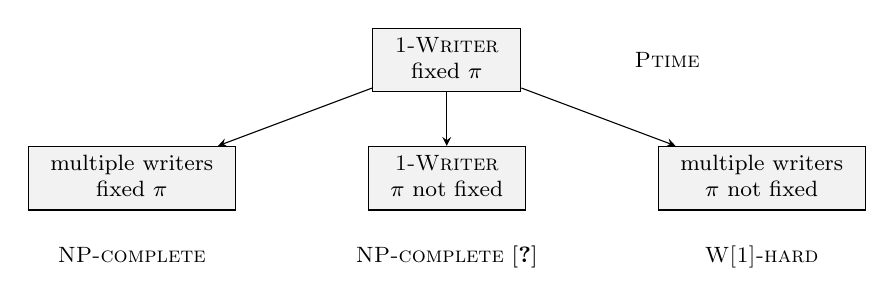
\begin{tikzpicture}[box/.style={rectangle, fill=gray!10, draw, inner sep=2pt}]
  \node[box] (a) at (0,0) {\footnotesize \begin{tabular}{c} \onewriter \\ fixed $\pp$ \end{tabular}};
  \node[box] (b) at (-4,-1.5) {\footnotesize \begin{tabular}{c} multiple writers \\ fixed $\pp$ \end{tabular}};
  \node[box] (c) at (0, -1.5) {\footnotesize \begin{tabular}{c} \onewriter \\ $\pp$ not fixed \end{tabular}};
  \node[box] (d) at (4, -1.5) {\footnotesize \begin{tabular}{c} multiple writers \\ $\pp$ not fixed \end{tabular}};
  
  \begin{scope}[->]
    \draw (a) to (b);
    \draw (a) to (c);
    \draw (a) to (d);
  \end{scope}
 
  \node at (2.8, 0) {\footnotesize \textsc{Ptime} };
  \node at (-4, -2.5) {\footnotesize \begin{tabular}{c} \textsc{NP-complete}  \\  \end{tabular}};
  \node at (0, -2.5) {\footnotesize \textsc{NP-complete}~\cite{gibbons}};
  \node at (4, -2.5) {\footnotesize \begin{tabular}{c} \textsc{W[1]-hard} \\ \end{tabular}}; 
\end{tikzpicture}
\caption{Illustration of the various complexity results}
\label{fig:results-overview}
\end{figure}

We shall discuss the complexity results when multiple writer programs are involved and what happens when $\pp$ is an input parameter. 

\paragraph*{Multiple writers, fixed $\pp$.} When multiple writers are allowed, \vscp\ becomes $\np$-complete, even with \twowriter\ programs (Theorem~\ref{th:NPhardness}). Furthermore, under the Exponential-Time-Hypothesis~\cite{ImpagliazzoPZ01}, we prove that VSC$^\pp$ cannot have a $2^{o(k)} \cdot n^{\mathcal{O}(1)}$ algorithm, even for $0$ preemptions and \threewriter\ programs (Theorem~\ref{th:Finegrained}). Contrast this with \onewriter\ where the exponent on $k$ was a constant $1$, thanks to the conflict analysis. Our hardness results therefore give strong evidence that the presence of multiple writers may introduce an unavoidable exponential on the number of threads $k$. 

\paragraph*{One writer, $\pp$ not fixed.} Now, if we continue with \onewriter\ but assume that $\pp$ is also part of the instance input, then Theorem~4.3 of \cite{gibbons} shows $\NP$-completeness. In their proof, an instance of 3-CNF-SAT with $k$ variables and $m$ clauses is reduced to a \onewriter\ program, where $\pp$ can be taken to be $\mathcal{O}(m + k)$. This is sufficient to prove $\NP$-hardness, when $\pp$ is not fixed. This hardness result provides evidence that having either $n^\pp$ or $k^\pp$ or some exponential function with $\pp$ could be unavoidable -- in our algorithm for Section~\ref{sec:one-writer}, we have $n^\pp$ and $\pp!$ in the running time. 

\paragraph*{Multiple writers, $\pp$ not fixed.} Finally, when we consider multiple writers, and do not fix $\pp$, we show W[1]-hardness (Section~\ref{sec:w1-hard}). W[1] is a complexity class studied in parameterized complexity, which intuitively provides evidence that we cannot have an algorithm with running time $f(\pp) \cdot (k + n)^{\mathcal{O}(1)}$ for our problem when multiple writers are allowed. In other words, we cannot separate out the influence of $\pp$ from $n$ and $k$. In contrast, consider the standard \emph{vertex cover} problem for graphs: given a graph of size $n$ is there a vertex cover of size $\le k$? This is an $\NP$-complete problem, but it has an algorithm of the form $f(k) \cdot n^{\mathcal{O}(1)}$ and hence is called fixed-parameter-tractable (FPT). On the other hand, deciding whether a graph of size $n$ has an \emph{independent set} of size $\ge k$ is known to be W[1]-hard (hence unlikely to be FPT). In Section~\ref{sec:w1-hard}, we reduce the independent set problem to our VSC problem, where the $k$ of the independent set translates to the $\pp$ of our VSC problem. We refer the reader to~\cite{DowneyFellows1999} for an exposition of parameterized complexity classes.

We divide the chapter into three sections. In the firts  begin by showing hardness result for \twowriter{}. The following section gives a lower bound result for \threewriter{} programs assuming ETH. In the last section of this chapter we shall show how the complexity of VSC$^\pp$ becomes \textsc{W[1]}-hard when $\pp$ is a parameter of the problem and not fixed. The results from this chapter are the following

\begin{restatable}{theorem}{scFinegrained}\label{th:Finegrained}
Under ETH, there is no $2^{o(k)} \cdot n^{\mathcal{O}(1)}$ algorithm for \vscp where $k$ is the number of threads, $n$ is the total number of operations.

The result holds even when the input instance is a \threewriter\ program.
\end{restatable}

\begin{restatable}{theorem}{scFinegrained}\label{th:NPhardness}
\vscp is $\NP$-complete, for all $\pi \ge 0$. Hardness holds even for \twowriter\ programs. 
\end{restatable}

\begin{restatable}{theorem}{wonehardness}\label{thm:w1-hard}
When $\pp$ is not fixed, and is treated as a parameter in the input, the \vscp\ problem is W[1]-hard.
\end{restatable} 
 


In the last chapter we have encountered how the VSC$^\pp$-problem becomes tractable for \onewriter{} programs with a complexity $\mathcal{O}(n^{\pp + 1} \cdot k \cdot \pp \cdot \pp!)$. Here are two observations about this complexity: the exponent on $k$ is a constant, whereas the exponent on $n$ is the parameter $\pp$. We remark that to achieve the polynomial-time complexity, we had restricted to \onewriter{}  programs and also assumed that the parameter $\pp$ is fixed. 

Our goal in this chapter is to investigate what happens when we perturb these restrictions. Figure~\ref{fig:results-overview} presents an overview of the complexity results.

\begin{figure}[h]
\centering
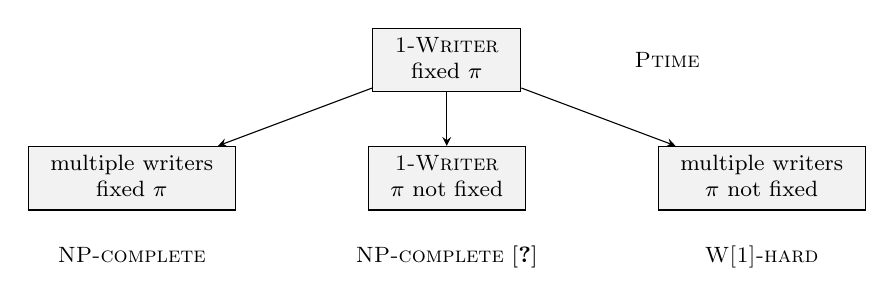
\begin{tikzpicture}[box/.style={rectangle, fill=gray!10, draw, inner sep=2pt}]
  \node[box] (a) at (0,0) {\footnotesize \begin{tabular}{c} \onewriter \\ fixed $\pp$ \end{tabular}};
  \node[box] (b) at (-4,-1.5) {\footnotesize \begin{tabular}{c} multiple writers \\ fixed $\pp$ \end{tabular}};
  \node[box] (c) at (0, -1.5) {\footnotesize \begin{tabular}{c} \onewriter \\ $\pp$ not fixed \end{tabular}};
  \node[box] (d) at (4, -1.5) {\footnotesize \begin{tabular}{c} multiple writers \\ $\pp$ not fixed \end{tabular}};
  
  \begin{scope}[->]
    \draw (a) to (b);
    \draw (a) to (c);
    \draw (a) to (d);
  \end{scope}
 
  \node at (2.8, 0) {\footnotesize \textsc{Ptime} };
  \node at (-4, -2.5) {\footnotesize \begin{tabular}{c} \textsc{NP-complete}  \\  \end{tabular}};
  \node at (0, -2.5) {\footnotesize \textsc{NP-complete}~\cite{gibbons}};
  \node at (4, -2.5) {\footnotesize \begin{tabular}{c} \textsc{W[1]-hard} \\ \end{tabular}}; 
\end{tikzpicture}
\caption{Illustration of the various complexity results}
\label{fig:results-overview}
\end{figure}

We shall discuss the complexity results when multiple writer programs are involved and what happens when $\pp$ is an input parameter. 

\paragraph*{Multiple writers, fixed $\pp$.} When multiple writers are allowed, \vscp\ becomes $\np$-complete, even with \twowriter\ programs (Theorem~\ref{th:NPhardness}). Furthermore, under the Exponential-Time-Hypothesis~\cite{ImpagliazzoPZ01}, we prove that VSC$^\pp$ cannot have a $2^{o(k)} \cdot n^{\mathcal{O}(1)}$ algorithm, even for $0$ preemptions and \threewriter\ programs (Theorem~\ref{th:Finegrained}). Contrast this with \onewriter\ where the exponent on $k$ was a constant $1$, thanks to the conflict analysis. Our hardness results therefore give strong evidence that the presence of multiple writers may introduce an unavoidable exponential on the number of threads $k$. 

\paragraph*{One writer, $\pp$ not fixed.} Now, if we continue with \onewriter\ but assume that $\pp$ is also part of the instance input, then Theorem~4.3 of \cite{gibbons} shows $\NP$-completeness. In their proof, an instance of 3-CNF-SAT with $k$ variables and $m$ clauses is reduced to a \onewriter\ program, where $\pp$ can be taken to be $\mathcal{O}(m + k)$. This is sufficient to prove $\NP$-hardness, when $\pp$ is not fixed. This hardness result provides evidence that having either $n^\pp$ or $k^\pp$ or some exponential function with $\pp$ could be unavoidable -- in our algorithm for Section~\ref{sec:one-writer}, we have $n^\pp$ and $\pp!$ in the running time. 

\paragraph*{Multiple writers, $\pp$ not fixed.} Finally, when we consider multiple writers, and do not fix $\pp$, we show W[1]-hardness (Section~\ref{sec:w1-hard}). W[1] is a complexity class studied in parameterized complexity, which intuitively provides evidence that we cannot have an algorithm with running time $f(\pp) \cdot (k + n)^{\mathcal{O}(1)}$ for our problem when multiple writers are allowed. In other words, we cannot separate out the influence of $\pp$ from $n$ and $k$. In contrast, consider the standard \emph{vertex cover} problem for graphs: given a graph of size $n$ is there a vertex cover of size $\le k$? This is an $\NP$-complete problem, but it has an algorithm of the form $f(k) \cdot n^{\mathcal{O}(1)}$ and hence is called fixed-parameter-tractable (FPT). On the other hand, deciding whether a graph of size $n$ has an \emph{independent set} of size $\ge k$ is known to be W[1]-hard (hence unlikely to be FPT). In Section~\ref{sec:w1-hard}, we reduce the independent set problem to our VSC problem, where the $k$ of the independent set translates to the $\pp$ of our VSC problem. We refer the reader to~\cite{DowneyFellows1999} for an exposition of parameterized complexity classes.

We divide the chapter into three sections. In the firts  begin by showing hardness result for \twowriter{}. The following section gives a lower bound result for \threewriter{} programs assuming ETH. In the last section of this chapter we shall show how the complexity of VSC$^\pp$ becomes \textsc{W[1]}-hard when $\pp$ is a parameter of the problem and not fixed. The results from this chapter are the following

\begin{restatable}{theorem}{scFinegrained}\label{th:Finegrained}
Under ETH, there is no $2^{o(k)} \cdot n^{\mathcal{O}(1)}$ algorithm for \vscp where $k$ is the number of threads, $n$ is the total number of operations.

The result holds even when the input instance is a \threewriter\ program.
\end{restatable}

\begin{restatable}{theorem}{scFinegrained}\label{th:NPhardness}
\vscp is $\NP$-complete, for all $\pi \ge 0$. Hardness holds even for \twowriter\ programs. 
\end{restatable}

\begin{restatable}{theorem}{wonehardness}\label{thm:w1-hard}
When $\pp$ is not fixed, and is treated as a parameter in the input, the \vscp\ problem is W[1]-hard.
\end{restatable} 
We now move on to present the hardness results. Firstly, we note that \vscp\ is in $\NP$, since we can guess an interleaving and check sequential consistency and the preemption bound $\pp$ in linear time. 
We present two hardness results for the case of fixed $\pp$. To show hardness, we provide reductions from 3-CNF-SAT. Given a Boolean formula $\varphi$ over variables $x_1, \dots, x_k$ and clauses $C_1, \dots, C_m$, where each clause is a disjunction of three literals, we ask whether $\varphi$ admits a satisfying assignment. We will start with the reduction to \threewriter\ systems and then adapt the reduction to \twowriter\ systems. The constructions for both the reductions are adapted from Theorem 2.1 of~\cite{Gibbons}. Let us first recall the Exponential Time Hypothesis that we make use of, to deduce a conditional lower bound.



\textbf{Exponential Time Hypothesis (ETH).}~\cite{ImpagliazzoPZ01}
There is no $2^{o(k)}\cdot (k+m)^{\mathcal{O}(1)}$ algorithm for 3-CNF-SAT, where $k$ is the number of variables and $m$ is the number of clauses.



For the reduction to $\threewriter$, we construct a concurrent program consisting of $\mathcal{O}(k)$ threads, i.e., linear in the number of variables of the 3-CNF-SAT instance, and no dependence on the number of clauses $m$. This yields a parameterized reduction and implies the desired conditional lower bound under ETH. In contrast, the reduction to $\twowriter$ uses $\mathcal{O}(k+m)$ threads and is therefore, not a parameterized reduction. Sections~\ref{sec:finegrained} and~\ref{sec:np} describe these reductions in detail.

\paragraph{Notation.}
Let $\varphi$ be a 3-CNF formula over variables $x_1, \dots, x_k$ and clauses $C_1, \dots, C_m$. Each clause $C_j$ consists of three literals $(\ell_j^1, \ell_j^2, \ell_j^3)$, where each literal is either a variable $x_i$ or its negation $\neg x_i$.

For each variable $x_i$, define:
\[
S_{x_i} := \{ j \mid C_j \text{ contains } x_i \}, \qquad
S_{\neg x_i} := \{ j \mid C_j \text{ contains } \neg x_i \}.
\]

Note that for ease of presentation, we omit thread identifiers in events when they are clear from the context.


\section{Fine-grained Hardness under ETH for \threewriter}\label{sec:finegrained}

Given a 3-CNF-SAT instance $\varphi$ in $k$ variable and $m$ clauses, we  construct a \vscp~ instance $\program$ in $\mathcal{O}(k)$ threads and $\mathcal{O}(k+m)$ operations, in $\mathcal{O}(k + m)$ time, such that for every variable only three threads write to it. Therefore, a $2^{o(k)} \cdot n^{\mathcal{O}(1)}$ algorithm for \vscp\ would contradict ETH.
 
\scFinegrained*


Say $\varphi=C_1\land C_2\land \dots \land C_m$. 
The construction for the reduction from $\varphi$, illustrated in Table~\ref{tab:reduction-threads-scmm} shows a program $\program_{\varphi}$ with $6k+1$ threads and $k+m+1$ variables. Variables $v_i, i=1,2,\dots,k$ correspond to $k$ variables of $\varphi$ while variables $c_i, i=1,2,\dots m$ correspond to the clauses. The variable $x$ is a guard to ensure all clause variables $c_i$ are set. Variable $x$ is written only once in $S_f$ while threads writing to $v_i$ are $S_i^0$ and $S_i^1$. Variable $c_i$ is written by $S_{x_i}$ if the clause $C_i$ contains $x$. If clause $C_i$ contains $\neg v_i$, then $c_i$ is written by $S_{\neg x_i}$. As a clause can have at most 3 literals in a 3-CNF-SAT instance, each $c_i$ will be written by at most 3 threads (hence we get a \threewriter\ program). We also pick $\pp$ to be $0$.

\begin{table}[h]
    \caption{Threads in the reduction to \threewriter\ programs}
    \label{tab:reduction-threads-scmm}
    \noindent
    \begin{minipage}{0.38\textwidth}
    \centering
    \begin{tabular}{c | c | c | c}
        $S_i^0$ & $H_i^0$ & $S_i^1$ & $H_i^1$ \\
        $\wt(v_i, 0)$ & $\rd(x, 1)$ & $\wt(v_i, 1)$ & $\rd(x, 1)$ \\
        & $\rd(v_i, 0)$ & & $\rd(v_i, 1)$ 
    \end{tabular}
    \end{minipage}
    \hfill
    \begin{minipage}{0.32\textwidth}
    \centering
    \begin{tabular}{c | c }
        $S_{x_i}$ & $S_{\neg x_i}$ \\
        $\rd(v_i, 1)$ & $\rd(v_i, 0)$ \\
        $\wt(c_j, 1)$ & $\wt(c_j, 1)$ \\
        $\forall j \in C_{x_i}$ & $\forall j \in C_{\neg x_i}$ 
    \end{tabular}
    \end{minipage}
    \hfill
    \begin{minipage}{0.22\textwidth}
    \centering
    \begin{tabular}{c}
        $S_f$ \\
        $\rd(c_1, 1)$ \\
        $\cdots$ \\
        $\rd(c_m, 1)$ \\
        $\wt(x, 1)$
    \end{tabular}
    \end{minipage}
\end{table}

Here is the main idea. In any (complete) $0$-preemption interleaving of $\program_\varphi$, the \emph{helper} threads $H_i^0$ and $H_i^1$ can be executed only after $S_f$ (due to the read-write on variable $x$). This ensures that only one of $S_i^0$ or $S_i^1$ can be executed before $S_f$: otherwise, if both are executed above $S_f$, only the helper thread corresponding to the last write on $v_i$ can be executed after $S_f$. Therefore, since a unique thread between $S_i^0$ or $S_i^1$ appears before $S_f$, we obtain an assignment for the variables. Moreover, as all the clauses have been set to true (thanks to $\rd(c_i, 1)$ in $S_f$), we can conclude that the assignment is satisfying. This leads to the following lemma.

\begin{restatable}{lemma}{threeWriterLemma}\label{lem:eth-sc}
    $\varphi$ is satisfiable iff there exists a sequentially consistent partial interleaving $\sigma$ of $\program_\varphi$ with $0$ preemptions.
\end{restatable}

\begin{proof}
    ($\Rightarrow$)
    Suppose $A$ is a satisfying assignment for $\varphi$. We construct a partial interleaving $\sigma$ as follows. Note that since we want $\sigma$ to have $0$ preemptions, each thread appears as a contiguous block.

    First, for each variable $x_i$, add the events of the thread $S^{A(x_i)}$, in some arbitrary order over $i$. 
    Next, for each $i$, add the thread $S_{x_i}$ if $A(x_i)=1$, and include $S_{\neg x_i}$ if $A(x_i)=0$. 
%    Note that since $\sigma$ has $0$ preemptions, each thread appears as a contiguous block.
%   Again, these threads are appended as contiguous blocks in $\sigma$.
    Since $A$ satisfies $\varphi$, for every clause $C_j$, at least one of the above threads writes $\wt(c_j,1)$ before any read of $c_j$ occurs (see Table~\ref{tab:reduction-threads-scmm}).
    Now add the thread $S_f$ to the interleaving. 
    By construction, for each read $\rd(c_j,1)$ in $S_f$, there is a preceding write $\wt(c_j,1)$ in $\sigma$ with no intervening conflicting write. Therefore, these reads respect the $\scmm$ semantics. The final write $\wt(x,1)$ in $S_f$ ensures that subsequent reads on $x$ read the value $1$.

    Next, for each $i$, add the helper thread $H_i^{A(x_i)}$. 
    Each such thread contains a read $\rd(x,1)$, which reads the value written by the write $\wt(x,1)$ in $S_f$, and a read $\rd(v_i, A(x_i))$, which reads the value written by  the earlier write in $S_i^{A(x_i)}$.
    Finally, add the remaining threads: for each $i$, include $S_i^{\neg A(x_i)}$, $H_i^{\neg A(x_i)}$, and the literal thread corresponding to the negation of $A(x_i)$. All reads in these threads reads the value written by earlier writes in $\sigma$.

    By construction, every read in $\sigma$ has the value written by the most recent preceding write to the same variable with the same value. Hence, $\sigma$ is sequentially consistent. Further, since each thread appears as a contiguous block, $\sigma$ has $0$ preemptions.

    ($\Leftarrow$) Suppose there exists a sequentially consistent partial interleaving $\sigma$ of $\program_\varphi$ with $0$ preemptions.
    Since $\sigma$ has $0$ preemptions, $\sigma$ is essentially just a concatenation of the threads in some order. 

    Each helper thread $H_i^0$ and $H_i^1$ contains a read $\rd(x,1)$, and hence must appear after the write $\wt(x,1)$ in $S_f$.

    Consider a variable $x_i$. If both $S_i^0$ and $S_i^1$ appear before $S_f$ in $\sigma$, then both $\wt(v_i,0)$ and $\wt(v_i,1)$ occur before $S_f$. Since no further writes to $v_i$ occur before the helper threads, only one of the reads $\rd(v_i,0)$ or $\rd(v_i,1)$ can have a preceding matching write with no intervening conflicting write. Thus, at most one of $H_i^0$ or $H_i^1$ can appear after $S_f$, contradicting completeness of $\sigma$. Hence, for each $i$, at most one of $S_i^0$ or $S_i^1$ appears before $S_f$.

From the construction of $\sigma$, we obtain the following assignment
\[
A(x_i) =
\begin{cases}
0 & \text{if } S_i^0 \text{ appears before } S_f \text{ in } \sigma,\\
1 & \text{otherwise.}
\end{cases}
\]
Now consider any clause $C_j$. The read $\rd(c_j,1)$ in $S_f$ requires a preceding write $\wt(c_j,1)$ in $\sigma$ with no intervening conflicting write. Such a write can only come from a thread corresponding to a literal of $C_j$ scheduled before $S_f$. By definition of $A$, this literal evaluates to true. Thus, each clause of $\varphi$ is satisfied.
\end{proof}



\section{NP-Hardness for \twowriter}\label{sec:np}

Here, our objective is to prove hardness even when at most two threads write to each variable. We reduce 3-CNF-SAT to \vscp\ for \twowriter\ programs. In this reduction, a formula $\varphi$ with $k$ variables and $m$ clauses yields a program $\program_\varphi$ with $\mathcal{O}(k+m)$ threads. While this suffices to show $\NP$-hardness, it does not yield the stronger ETH-based lower bound, which requires $\mathcal{O}(k)$ threads (and that does not depend on the number of clauses $m$).


The key challenge here is to reduce the number of threads writing to each clause variable $c_j$ from three (one for each literal in the clause) to at most two, while still encoding the satisfiability of the 3-CNF formula.
For each clause $C_j = (\ell_j^1 \vee \ell_j^2 \vee \ell_j^3)$, we introduce an additional auxiliary variable $d_j$, and modify the construction as follows.

\begin{itemize}[left=0.5em]
\item In the thread corresponding to the third literal $\ell_j^3$, replace the write $\wt(c_j,1)$ with $\wt(d_j,1)$.
\item Introduce a new thread with two events as follows:
\[
S_j = (j : \rd(c_j,1)) \cdot (j : \wt(d_j,1)).
\]
\item In the thread $S_f$, replace each $\rd(c_j,1)$ with $\rd(d_j,1)$.
\end{itemize}

This results in the same outcome. Either clause $C_j$ is set to true due to the third literal (and hence $\wt(d_j, 1)$ happens), or if it needs to be true due to the first or second literal, then $S_j$ comes into effect and performs $\wt(d_j, 1)$.
Let $\program_\varphi$ denote the resulting program. Note that due to the additional threads $S_j$, the total number of threads now also depends on $m$, the number of clauses. 


\begin{restatable}{lemma}{twoWriterLemma}\label{lem:np-two-writer}
$\varphi$ is satisfiable iff there exists a sequentially consistent partial interleaving $\sigma$ of $\program_\varphi$ with $0$ preemptions.
\end{restatable}

\begin{proof}
    The proof follows the same structure as Lemma~\ref{lem:eth-sc}.

    ($\Rightarrow$) Suppose that $A$ is a satisfying assignment for $\varphi$. We construct a partial interleaving $\sigma$ with $0$ preemptions.
    For each variable $x_i$, add the thread $S_i^{A(x_i)}$ and the corresponding literal thread ($S_{x_i}$ if $A(x_i)=1$, otherwise $S_{\neg x_i}$).

    Now, consider a clause $C_j$. If the third literal $\ell_j^3$ is true under $A$, include the thread corresponding to $\ell_j^3$ before $S_f$. Then the write $\wt(d_j,1)$ appears before $S_f$, and the read $\rd(d_j,1)$ in $S_f$ is satisfied.
    Otherwise, one of $\ell_j^1$ or $\ell_j^2$ is true. 
    Include the corresponding literal thread (which writes $\wt(c_j,1)$), followed by $S_j$. Then the read $\rd(c_j,1)$ in $S_j$ has a preceding write with no intervening conflicting write, and $\wt(d_j,1)$ in $S_j$ appears before $S_f$.
    After handling all clauses, add the thread $S_f$. Finally, add all remaining threads. By construction, each read has a preceding matching write with no intervening conflicting write, and $\sigma$ has $0$ preemptions.

\medskip

    ($\Leftarrow$) Suppose there exists a sequentially consistent partial interleaving $\sigma$ with $0$ preemptions. Then $\sigma$ is a concatenation of threads. As in Lemma~\ref{lem:eth-sc}, for each variable $x_i$, at most one of $S_i^0$ or $S_i^1$ appears before $S_f$. Define
\[
A(x_i) =
\begin{cases}
0 & \text{if } S_{i}^0 \text{ appears before } S_f,\\
1 & \text{otherwise.}
\end{cases}
\]

    Consider a clause $C_j$. The read $\rd(d_j,1)$ in $S_f$ must have a preceding write $\wt(d_j,1)$ in $\sigma$ with no intervening conflicting writes. This write can either copme from the thread corresponding to $\ell_j^3$, or from $S_{j}$. If it comes from the thread for $\ell_j^3$, then that thread appears before $S_f$, and hence $\ell_j^3$ evaluates to true under $A$.
    Otherwise, it comes from $S_{j}$. In this case, the read $\rd(c_j,1)$ in $S_{j}$ must have a preceding write $\wt(c_j,1)$ in a literal thread corresponding to $\ell_j^1$ or $\ell_j^2$ that appears before $S_{j}$, and hence before $S_f$. The corresponding literal is therefore true under $A$.

    Thus, in all cases, at least one literal in $C_j$ is true under $A$. Hence $\varphi$ is satisfiable.\qedhere
\end{proof}






Thus, we have shown that the preemption-bounded consistency problem is $\NP$-hard for \twowriter~programs. 



%%%%%%%%%%%%
%%%%%%%%%%%%

\section{W[1]-hardness for VSC$^\pp$ when $\pp$ is an input parameter}\label{sec:w1-hard}


In parameterized complexity, W-hierarchy is a well-known concept. It helps organize parameterized problems according to their level of difficulty. One can refer to  \cite{DowneyFellows1999} for a clear understanding. As discussed earlier, it is believed that $\textsc{FPT} \neq W[1]$. One well known problem in the $W[1]$ class is the $k$-independent set problem.

\textbf{$k$-independent set problem}: Let $G = (V,E)$ be a connected graph with vertex set $V$ and edge set $E$. The $k$-independent set problem asks if there exists a set of vertices $V_k \subseteq V$ of size $k$ such that no two vertices share a common edge.

We will use parameterized reduction to reduce an instance $(G, k)$ of the independent set problem to an instance $(\program_G, \pp)$ with $\pp = 3k$, of the \vscp\ problem and prove the following theorem. 

\wonehardness*


\paragraph*{Construction.} The program $\program_G$ is depicted in Table~\ref{tab:independent-set}. It has an $\Init$ thread, $k$ checker threads $\Checker_1, \Checker_2, \dots, \Checker_k$, and $k$ selector threads $\Sel_1, \Sel_2, \dots, \Sel_k$. There is a variable $y_e$ corresponding to each edge $e \in E$, variables $x_1, x_2, \dots, x_k$ to help pick $k$ vertices, and some book-keeping variables $s, p_0, \dots, p_k$. Figure \ref{fig:Example-w1} may  enhance the understanding of the the construction. The graph at the bottom right of the figure has three vertices \circl{1}, \circl{2} and \circl{3} with edges between \circl{1}, \circl{2} and \circl{2}, \circl{3}. The corresponding edge  varibles are $y_{12}$ and $y_{23}$. We have assumed $k=2$. Hence,  there are two selector threads $S_1$, $S_2$, two checker threads and two variables $x_1$ and $x_2$ to help select a vertex set of size 2 as discussed earlier.



\begin{figure}[!htbp]
    %\begin{wrapfigure}[32]{l}{0.5\columnwidth}
        %\resizebox{0.5\columnwidth}{!}{%
        \newcommand{\xdisposition}{0}
        \newcommand{\ydisposition}{0}
        \newcommand{\xtstep}{0.3}
        \newcommand{\ytstep}{0.7}
        \newcommand{\ybias}{-0.3 }
        \newcommand{\xstep}{2}
        \newcommand{\ystep}{-0.6}
        \newcommand{\xtscale}{0.8}
        \def\crossoutopacity{0.3}
        \def \numevents{29}
        \def\scale{0.8}
        \centering
    %    \resizebox{\columnwidth}{!}{%
        \begin{tikzpicture}[thick, font=\footnotesize,
        pre/.style={<-,shorten >= 2pt, shorten <=2pt, very thick},
        post/.style={->,shorten >= 3pt, shorten <=3pt,   thick},
        seqtrace/.style={line width=1},
        und/.style={very thick, draw=gray},
        virt/.style={circle,draw=black!50,fill=black!20, opacity=0}]
    
        \tikzstyle{event} = [rectangle, fill=white, inner sep=0, minimum height=4.6mm, minimum width=25mm, rounded corners]
    
    
        \node[] (S11) at (.5*\xstep,2*\ystep) {\normalsize $\Sel_{1}$};
        \node[] (S12) at (.5*\xstep,\numevents*\ystep) {};
        \draw[seqtrace] (S11) to (S12);
     
        \node[] (S21) at (2*\xstep,2*\ystep) {\normalsize $\Sel_{2}$};
        \node[] (S22) at (2*\xstep,\numevents*\ystep) {};
        
        
         \draw[seqtrace] (S21) to (S22);
         
    %%%%S1%%%%
       % \node[event, draw=black] (11) at (.5*\xstep, 1*\ystep + 0*\ybias) {$\rd(s, \top)$};
    
        \node[event, draw=green] (12) at (.5*\xstep, 3*\ystep + 0*\ybias) {$\rd(y_{12}, 0)$};
         \node[event, draw=green] (13) at (.5*\xstep, 4*\ystep + 0*\ybias) {$\wt(y_{12}, 1)$};
        
        \node[event, draw=black] (14) at (.5*\xstep, 5*\ystep + 0*\ybias) {$\rd(s, 1)$};
        \node[event, draw=black] (15) at (.5*\xstep, 6*\ystep + 0*\ybias) {$\wt(x_1, 0)$};
        \node[event, draw=black] (16) at (.5*\xstep, 7*\ystep + 0*\ybias) {$\wt(x_1, 1)$};
        
        \node[event, draw=green] (17) at (.5*\xstep, 8*\ystep + 0*\ybias) {$\rd(y_{12},1)$};
        \node[event, draw=green] (18) at (.5*\xstep, 9*\ystep + 0*\ybias) {$\wt(y_{12},0)$};
        
        
    
        \node[event, draw=red] (19) at (.5*\xstep, 11*\ystep + 0*\ybias) {$\rd(y_{12}, 0)$};
        \node[event, draw=red] (20) at (.5*\xstep, 12*\ystep + 0*\ybias) {$\wt(y_{12}, 1)$};
        \node[event, draw=red] (21) at (.5*\xstep, 13*\ystep + 0*\ybias) {$\rd(y_{23}, 0)$};
        \node[event, draw=red] (22) at (.5*\xstep, 14*\ystep + 0*\ybias) {$\wt(y_{23}, 1)$};
        
        
        
        
        
        \node[event, draw=black] (23) at (.5*\xstep, 15*\ystep + 0*\ybias) {$\rd(s, 1)$};
        \node[event, draw=black] (24) at (.5*\xstep, 16*\ystep + 0*\ybias) {$\wt(x_1, 0)$};
        \node[event, draw=black] (25) at (.5*\xstep, 17*\ystep + 0*\ybias) {$\wt(x_1, 1)$};
        
        
        \node[event, draw=red] (26) at (.5*\xstep, 18*\ystep + 0*\ybias) {$\rd(y_{12}, 1)$};
        \node[event, draw=red] (27) at (.5*\xstep, 19*\ystep + 0*\ybias) {$\wt(y_{12}, 0)$};
        \node[event, draw=red] (28) at (.5*\xstep, 20*\ystep + 0*\ybias) {$\rd(y_{23}, 1)$};
        \node[event, draw=red] (29) at (.5*\xstep, 21*\ystep + 0*\ybias) {$\wt(y_{23}, 0)$};
        
        
        
       \node[event, draw=blue] (31) at (.5*\xstep, 23*\ystep + 0*\ybias) {$\rd(y_{23}, 0)$};
        \node[event, draw=blue] (32) at (.5*\xstep, 24*\ystep + 0*\ybias) {$\wt(y_{23}, 1)$};
        \node[event, draw=black] (33) at (.5*\xstep, 25*\ystep + 0*\ybias) {$\rd(s, 1)$};
        \node[event, draw=black] (34) at (.5*\xstep, 26*\ystep + 0*\ybias) {$\wt(x_1, 0)$};
        \node[event, draw=black] (35) at (.5*\xstep, 27*\ystep + 0*\ybias) {$\wt(x_1, 1)$};\node[event, draw=blue] (36) at (.5*\xstep, 28*\ystep + 0*\ybias) {$\rd(y_{23}, 1)$};
        \node[event, draw=blue] (37) at (.5*\xstep, 29*\ystep + 0*\ybias) {$\wt(y_{23}, 0)$};
    
       
    %%%%S2%%%%%
    
    
    % \node[event, draw=black] (11) at (2*\xstep, 1*\ystep + 0*\ybias) {$\rd(s, \top)$};
    
        \node[event, draw=green] (12) at (2*\xstep, 3*\ystep + 0*\ybias) {$\rd(y_{12}, 0)$};
         \node[event, draw=green] (13) at (2*\xstep, 4*\ystep + 0*\ybias) {$\wt(y_{12}, 2)$};
        
        \node[event, draw=black] (14) at (2*\xstep, 5*\ystep + 0*\ybias) {$\rd(s, 1)$};
        \node[event, draw=black] (15) at (2*\xstep, 6*\ystep + 0*\ybias) {$\wt(x_2, 0)$};
        \node[event, draw=black] (16) at (2*\xstep, 7*\ystep + 0*\ybias) {$\wt(x_2, 1)$};
        
        \node[event, draw=green] (18) at (2*\xstep, 8*\ystep + 0*\ybias) {$\rd(y_{12},2)$};
        \node[event, draw=green] (19) at (2*\xstep, 9*\ystep + 0*\ybias) {$\wt(y_{12},0)$};
    
        \node[event, draw=red] (19) at (2*\xstep, 11*\ystep + 0*\ybias) {$\rd(y_{12}, 0)$};
        \node[event, draw=red] (20) at (2*\xstep, 12*\ystep + 0*\ybias) {$\wt(y_{12}, 2)$};
        
        \node[event, draw=red] (21) at (2*\xstep, 13*\ystep + 0*\ybias) {$\rd(y_{23}, 0)$};
       
        \node[event, draw=red] (22) at (2*\xstep, 14*\ystep + 0*\ybias) {$\wt(y_{23}, 2)$};
        
        \node[event, draw=black] (23) at (2*\xstep, 15*\ystep + 0*\ybias) {$\rd(s, 1)$};
        \node[event, draw=black] (24) at (2*\xstep, 16*\ystep + 0*\ybias) {$\wt(x_2, 0)$};
        \node[event, draw=black] (25) at (2*\xstep, 17*\ystep + 0*\ybias) {$\wt(x_2, 1)$};
        
        
        \node[event, draw=red] (26) at (2*\xstep, 18*\ystep + 0*\ybias) {$\rd(y_{12}, 2)$};
        \node[event, draw=red] (28) at (2*\xstep, 19*\ystep + 0*\ybias) {$\wt(y_{12}, 0)$};
        \node[event, draw=red] (29) at (2*\xstep, 20*\ystep + 0*\ybias) {$\rd(y_{23}, 2)$};
        \node[event, draw=red] (30) at (2*\xstep, 21*\ystep + 0*\ybias) {$\wt(y_{23}, 0)$};
        
        
       \node[event, draw=blue] (31) at (2*\xstep, 23*\ystep + 0*\ybias) {$\rd(y_{23}, 0)$};
        \node[event, draw=blue] (32) at (2*\xstep, 24*\ystep + 0*\ybias) {$\wt(y_{23}, 2)$};
        \node[event, draw=black] (33) at (2*\xstep, 25*\ystep + 0*\ybias) {$\rd(s, 1)$};
        \node[event, draw=black] (34) at (2*\xstep, 26*\ystep + 0*\ybias) {$\wt(x_2, 0)$};
        \node[event, draw=black] (35) at (2*\xstep, 27*\ystep + 0*\ybias) {$\wt(x_2, 1)$};
         \node[event, draw=blue] (36) at (2*\xstep, 28*\ystep + 0*\ybias) {$\rd(e_{23}, 2)$};
        \node[event, draw=blue] (37) at (2*\xstep, 29*\ystep + 0*\ybias) {$\wt(e_{23}, 0)$};
    
    %%%%%%%%%%%%%%%%%%%%%%%%%%%%%%%%%%%%%%%%%%%%%%%%%%%%%%
            
       
       \def \numevents{4}
      
       \begin{scope}[xshift=0cm,yshift=-2cm]
         
                \node[] (S11) at (3.5*\xstep,0) {\normalsize $\mathsf{Checker_1}$};
                \node[] (S12) at (3.5*\xstep, \numevents* \ystep) {};
            
                \draw[seqtrace] (S11) to (S12);
            
                
                \node[event, draw=black] (11) at (3.5*\xstep, 1*\ystep + 0*\ybias) {$\rd(p_{0}, 1)$};
                \node[event, draw=black] (12) at (3.5*\xstep, 2*\ystep + 0*\ybias) {$\wt(s, 0)$};
                
                \node[event, draw=black] (13) at (3.5*\xstep, 3*\ystep + 0*\ybias) {$\rd(x_1, 0)$};
                \node[event, draw=black] (13) at (3.5*\xstep, 4*\ystep + 0*\ybias) {$\wt(p_1, 1)$};
                
        
        \end{scope}
        
        \begin{scope}[xshift=0cm,yshift=-6cm]
         
                 \node[] (S11) at (3.5*\xstep,0) {\normalsize $\mathsf{Checker_2}$};
                \node[] (S12) at (3.5*\xstep, \numevents* \ystep) {};
            
                \draw[seqtrace] (S11) to (S12);
            
                
                \node[event, draw=black] (11) at (3.5*\xstep, 1*\ystep + 0*\ybias) {$\rd(p_{1}, 1)$};
              \node[event, draw=black] (12) at (3.5*\xstep, 2*\ystep + 0*\ybias) {$\rd(x_2, 0)$};                
                \node[event, draw=black] (13) at (3.5*\xstep, 3*\ystep + 0*\ybias) {$\wt(s, 1)$};                
                \node[event, draw=black] (13) at (3.5*\xstep, 4*\ystep + 0*\ybias) {$\wt(p_2, 1)$};
                
        
        \end{scope}
       
        
        \def \numevents{6}
          \begin{scope}[xshift=3cm,yshift=-2cm]
         
                \node[] (S11) at (3.5*\xstep,0) {\normalsize $\mathsf{Init}$};
                \node[] (S12) at (3.5*\xstep, \numevents* \ystep) {};
            
                \draw[seqtrace] (S11) to (S12);
            
                
                \node[event, draw=black] (11) at (3.5*\xstep, 1*\ystep + 0*\ybias) {$\wt(y_{12}, 0)$};
                \node[event, draw=black] (12) at (3.5*\xstep, 2*\ystep + 0*\ybias) {$\wt(y_{23}, 0)$};
                \node[event, draw=black] (13) at (3.5*\xstep, 3*\ystep + 0*\ybias) {$\wt(x_{1}, 1)$};
                \node[event, draw=black] (14) at (3.5*\xstep, 4*\ystep + 0*\ybias) {$\wt(x_2, 1)$};
                \node[event, draw=black] (15) at (3.5*\xstep, 5*\ystep + 0*\ybias) {$\wt(s, 1)$};
                \node[event, draw=black] (15) at (3.5*\xstep, 6*\ystep + 0*\ybias) {$\wt(p_0, 1)$};
        
        \end{scope}
        
    
                \begin{scope}[xshift=8cm,yshift=-10cm]
                \node[circle, draw=green, minimum size=.3cm] (1) {1};
                \node[circle, draw=red, minimum size=.3cm, right of=1] (2) {2};
                \node[circle, draw=blue, minimum size=.3cm, right of=2] (3) {3};
            
                % Edges
                \draw[-] (1) -- (2);
                \draw[-] (2) -- (3);
                \end{scope}
            
      
        \end{tikzpicture}   
        %}
        %}
        \caption{The $W[1]$-hardness reduction.}
        \label{fig:Example-w1}
    %\end{wrapfigure}
\end{figure}



 

\begin{table}
\centering
\caption{Reduction from $k$-independent set problem. Index $j$ ranges from $1$ to $k$.}
\label{tab:independent-set}
\medskip
\centering
\begin{tabular}{l  @{\qquad} l  @{\qquad} l }
    $\Init$ &  $\Checker_j$ & $~\Sel_j$ \\
    &  & \\
$\wt(y_e, 0)$   &  $\rd(p_{j-1}, 1)$ &   $\forall v \in V:$  \\
$\forall e \in E$  &  $\wt(s, 0)$ when $j \neq k$ &  \\
& & $\rd(y_e, 0);~\wt(y_e, j)$ \quad $\forall e \in E$ containing $v$ \\
$\wt(x_j, 1)$ &  $\rd(x_j, 0)$  &  \\
$\forall 1 \le j \le k$ & $\wt(s, 1)$ when $j = k$  & $\rd(s, 1)$   \\
  & &  $\wt(x_j, 0)$   \\
$\wt(s, 1)$ & $\wt(p_j, 1)$ &  $\wt(x_j, 1)$  \\
$\wt(p_0, 1)$ & &   \\
 & &   $\rd(y_e, j);~\wt(y_e, 0)$ \quad $\forall e \in E$ containing $v$  
\end{tabular}
\end{table}

The $\Init$ thread is self-explanatory from Table~\ref{tab:independent-set}. For the first $k-1$ checker threads $\Checker_j$ (with $1 \le j \le k-1$) the second operation is $\wt(s, 0)$ (depicted as $\wt(s,0)$ when $j \neq k$). These threads do not have a $\wt(s,1)$ instruction at all. For the last checker thread $\Checker_k$, there is no $\wt(s,0)$, and instead there is a $\wt(s, 1)$ right after $\rd(x_j, 0)$. 
with three blocks each corresponding to the three vertices of the given graph
We now explain the selector threads. Each selector thread $\Sel_j$  
has $|V|$ blocks of operations, one block for each $v \in V$. Taking $V = \{u_1, \dots, u_n\}$, the selector thread $\Sel_j$ can be seen as:
\begin{align*}
 \Sel_j: \quad \BB^j_{u_1}~ \BB^j_{u_2}~\cdots~ \BB^j_{u_n}
\end{align*} 
where each $B^j_u$ is a block of operations corresponding to a vertex $u$. This can further be seen as sub-blocks:
\begin{align*}
 \BB^j_u:~~&~  \Start^j_u ~~\rd(s, 1) ~~ \wt(x_j, 0) ~~ \wt(x_j, 1) ~~ \Finish^j_u \\
 \text{ where~} \qquad \qquad \Start^j_u: ~~& ~\rd(y_e, 0) ~ \wt(y_e, j) ~~ \forall e  \text{ incident on } u \\
\Finish^j_u: ~~& ~\rd(y_e, j) ~ \wt(y_e, 0) ~~ \forall e \text{ incident on } u
\end{align*}
Figure~\ref{fig:Example-w1} shows each selector thread with three blocks each, corresponding to the three vertices of the given graph. Example for vertex \circl{1}, $\Sel_1$ has the block 
 $$B_1^1:~\rd(y_{12},0) \wt(y_{12},1) \quad \rd(s,0) \wt(x_1,0) \wt(x_1,1) \quad \rd(y_{12},1) \wt(y_{12},0)$$
 

%%%%%%%%%correctness%%%%%%%%%

The correctness of the construction is explained through the next two lemmas.

\begin{lemma}\label{lem:independent-set-to-SC-interleaving}
If $G$ has an independent set of size $k$, there is an SC interleaving for $\program_G$ with $3k$ preemptions.
\end{lemma}
\begin{proof} 
Suppose $G$ has an independent set $\{v_1, v_2, \dots, v_k\}$ of size $k$. Then $\program_G$ will have $k$ selector threads. 
Consider an SC interleaving of $\program_G$. It begins with the execution of the $\Init$ thread. The checker and selector threads appear later. 
Notice two conflicting events: the $\Init$ thread has $\wt(x_j, 1)$ whereas $\Checker_j$ has a read $\rd(x_j, 0)$. Therefore, a $\wt(x_j, 0)$ has to appear somewhere in between. This can be provided by $\Sel_j$: for $\wt(x_j, 0)$ to be the last write between the conflicting events in $\Init$ and $\Checker_j$, a part of $\Sel_j$ ending at a $\wt(x_j,0)$ operation should appear in between. So, we say that $\Sel_j$ is ``inside'' some block corresponding to a vertex -- call this vertex $v_j$. Intuitively, we require every $\Sel_j$ to have executed upto a $\wt(x_j, 0)$, then wait for $\Checker_j$ to finish, and subequently execute the rest of $\Sel_j$ that starts with $\wt(x_j, 1)$. However, we cannot do this na\"ively. Suppose $\Sel_1$ executes upto $\wt(x_1,0)$ of $\BB^1_{v_1}$. Then at the start of this block, we have writes $\wt(y_e, 1)$ for all $e$ incident on $v_1$. This may disable the execution of $\Sel_2$ -- notice that the beginning of each block contains a read of the form $\rd(y_e, 0)$. Therefore we need to carefully reach to $\wt(x_j, 0)$ in each thread. We do this in phases. 

\begin{figure}[h]
\centering
\scalebox{0.85}{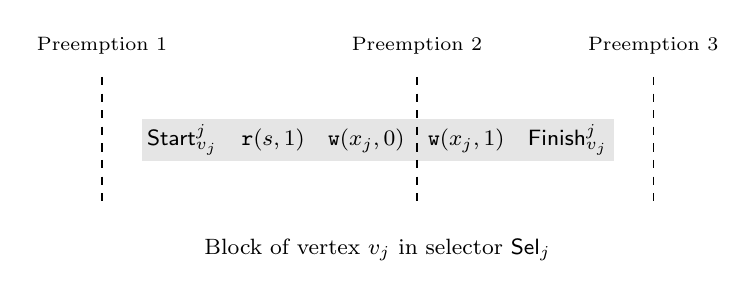
\begin{tikzpicture}[box/.style={rectangle, fill=gray!20, inner sep=2pt}]
\begin{scope}[every node/.style={box}]
  
  \node (b) at (4,0) {\footnotesize $\Start^j_{v_j}~$ $~\rd(s, 1)~$ $~\wt(x_j,0)~$ $~\wt(x_j, 1)~$ $~\Finish^j_{v_j}$ };
\end{scope}
\node at (4, -1.4) {\footnotesize Block of vertex $v_j$ in selector $\Sel_j$};
\draw [dashed] (0.5, 0.8) -- (0.5, -0.8);
\draw [dashed] (4.5, 0.8) -- (4.5, -0.8);
\draw [dashed] (7.5, 0.8) -- (7.5, -0.8);

\node at (0.5, 1.2) {\scriptsize  Preemption $1$};
\node at (4.5, 1.2) {\scriptsize  Preemption $2$};
\node at (7.5, 1.2) {\scriptsize  Preemption $3$};
\end{tikzpicture}}
\caption{Illustrating the preemption points within a selector thread}
\label{fig:w1-illustration}
\end{figure}

%%%%


\begin{description}
\item[Phase 0.] First execute $\Init$ completely.
\item[Phase 1.] We make all the selector threads execute upto the beginning of some block (see preemption $1$ in Figure~\ref{fig:w1-illustration}), one after the other. For example if $v_1=u_m$, execute $\Sel_1$ execute from $\BB^1_{u_1}$ upto $\BB^1_{u_{m-1}}$. Since the end of each block ``resets'' $y_e$ to $0$ (through the $\wt(y_e, 0)$ instruction), such an execution is possible. This phase incurs $k$ preemptions. 

\item[Phase 2.] As a second step, we make every selector $Sel_j$  execute upto $\wt(x_j, 0)$, that is, between preemption points $1$ and $2$ in Figure~\ref{fig:w1-illustration}. The crucial point is that this phase of executions is possible only when the selectors have picked an independent set: on executing $\Sel_j$ upto preemption point $2$, all $y_e$ for edges $e$ incident on $v_j$ have been set to $j$, but since none of these edges is incident on a $v_i$ ($i \neq j$), the selector thread $\Sel_i$ can also pass through its $\rd(y_{e'}, 0)$ operations and execute upto $\wt(x_i, 0)$. Again this phase ends with $k$ preemptions. 

%the $\rd(s,1)$ operation present in block $v_1$, then $\Sel_2$ upto $\rd(s_1)$ in block $v_2$, and so on until $\Sel_k$ upto $\rd(s, 1)$ of block $v_k$. There are $2k$ preemptions so far.
%\item Execute $\Sel_1$ upto $\wt(x_1, 0)$ of block $v_1$. All edges incident on $v_1$ now have a preceding $\wt(y_e, 1)$. Since we started with an independent set, none of these edges are incident on $v_2, \dots, v_k$. Similarly, we can execute $\Sel_2$ upto $\wt(x_2, 0)$, followed by $\Sel_3$, until we finish with $\Sel_k$ upto $\wt(x_k, 0)$. The fact that we started with an independent set allows to parallely execute all the blocks corresponding to $v_1, \dots, v_k$. In this phase, there are $k$ more preemptions.
\item[Phase 3.] Now, we completely execute $\Checker_1$, followed by $\Checker_2$, and so on, until $\Checker_k$. No extra preemptions get added. 
\item[Phase 4.] After all the $k$ checkers are executed, we want to execute the rest of the selector threads after the checker threads are completed. However, executing the full selector may not be possible since some of the $y_e$ variables have current values different from $0$. So to once again reset all $y_e$ to $0$, we execute each selector upto $\wt(y_e, 0)$ at end of the current block. Here we stand at the preemption point $3$ shown in Figure~\ref{fig:w1-illustration}. Total number of preemptions so far is $3k$.

\item[Phase 5. ] Finally, we can execute all the $\Sel_j$ threads one by one without incurring any preemptions. 
\end{description} 

This shows that when the selectors choose an independent set, an SC interleaving with at most $3k$ preemptions is possible, with $3$ preemptions occuring in each selector thread.

Also by construction, the interleaving is sequentially consistent. 
\end{proof}

\begin{lemma}\label{lem:sc-interleaving-to-independent-set}
If $\program_G$ has an SC interleaving, then $G$ has an independent set of size $k$.
\end{lemma}
\begin{proof} 

Suppose there is an SC interleaving of $\program_G$. Here are some observations.
\begin{itemize}
\item Before the $\rd(x_j, 0)$ event of $\Checker_j$, the last write on $x_j$ should be $\wt(x_j, 0)$. Hence $\Sel_j$ should have executed the operations inside some block $\BB^j_{v_j}$ upto $\wt(x_j, 0)$.  
%\item Due to the read $\rd(x_j, 0)$ in $\Checker_j$, the selector thread should be inside a block, and end at $\wt(x_j, 0)$ of some vertex $v_j$, before the $\rd(x_j,0)$.
\item Due to the $p_j$ variables, $\Checker_1$ executes completely before $\Checker_2$. Similarly, $\Checker_2$ executes completely before $\Checker_3$ starts, and so on.
\item Notice the $\wt(s, 0)$ in $\Checker_1$, and a $\rd(s, 1)$ in every block $\BB^j_{v_j}$. Since, (1) all instructions upto $\wt(x_j, 0)$ need to be done before $\Checker_j$, and (2) $\rd(s, 1)$ cannot happen after $\Checker_1$, we deduce that all the selectors have executed atleast upto $\rd(s, 1)$ before the $\wt(s,0)$ of $\Checker_1$. In particular, the block $\Start^j_{v_j}$ is executed before $\wt(s, 0)$ of $\Checker_1$.

%\item Due to the $\wt(s,0)$ in $\Checker_j$, for $j < k$, no selector thread can enter a block between $\Checker_j$ and $\Checker_{j+1}$: that is, the operation $\rd(s,1)$ and the statements above it in every selector should have been executed before $\Checker_1$ begins. 
\end{itemize} 
The crucial point is that: before the $\wt(s,0)$ of $\Checker_1$, we have executed the operation $\wt(y_e, j)$ for all edges incident on $v_j$, due to the block $\Start^j_{v_j}$. We claim that there can be no edge between $v_i$ and $v_j$ when $i \neq j$. Suppose there is an edge $e = (v_i, v_j)$ between two selected vertices. Firstly, when the checkers start executing, all selectors $S_l$ must be inside some block $B^l_{v_l}$. Thread $\Sel_i$ has a $\wt(y_e, i)$ and thread $\Sel_j$ has a $\wt(y_e, j)$ before $\wt(x_i, 0)$ and $\wt(x_j, 0)$ respectively. Notice the reads $\rd(y_e, i)$ in $\Sel_i$ and $\rd(y_e, j)$ in $\Sel_j$ in the $\Finish$ blocks,  which need to be executed, after the $\Checker$ threads. This would not be possible in an SC interleaving. We conclude that there can be no common edge between $v_i$ and $v_j$. This shows that the selected vertices form an independent set, of size $k$. 
\end{proof}

The two lemmas above prove the correctness of our reduction. If $G$ has an independent set of size $k$, we get an interleaving in $\program_G$ with $3k$ preemptions (Lemma~\ref{lem:independent-set-to-SC-interleaving}). If $\program_G$ has an SC interleaving with $3k$ preemptions, in particular, this means there is an SC interleaving. Lemma~\ref{lem:sc-interleaving-to-independent-set} shows there is an independent set of size $k$. 

\section{Discussion}

In the last two chapters, we have studied  the fundamental VSC-problem in the context of bounded preemptions. This is a deviation from the usual parameters
considered in the study of this problem. The results are two-fold: an algorithm
for the single-writer case, and hardness reductions in the presence of multiple
writers, and unbounded preemptions. On the algorithmic front, the key insight is
that for 1-Writer systems the idea of a conflict graph helps to determine order-
ing without having to fall back on a systematic enumeration of all permutations. 
Such a trick is not possible in the case of multiple writers.
In fact the problem seems harder with increase in number of writers. 


Investigating a preemption-bounded version of stateless model-checking under
the reads-value-from equivalence and the impact of incorporating the VSC $\pp$ problem into the procedure, remain directions for future work. Another interesting
direction is to investigate the consistency problem for the Total Store Ordering
(TSO) memory model under the influence of various context-switches \cite{TSO-context-bounding} defined
in the literature.



\endinput










%%%%%%%%%%%%%%%%%%%%%%%%%%%%%%%%%
 





 
\begin{center}
    \chapter*{\centering Part B}
    \addcontentsline{toc}{chapter}{\centering Part B} 
\end{center}
  


\chapter{Weak Memory Models}

Modern hardware and compilers apply various optimizations (like instruction reordering, store buffering, etc.) to enhance performance. These optimizations can cause threads to observe writes to a shared memory location in an order that differs from the program order. \emph{Memory models} formalize the rules to constrain which values reads may observe, and allow the programmer to be aware of the memory behaviour. In this chapter we shall discuss the formalization of certain fragments of C-11 memory models.   The relevant models are `release-acquire' ($\ramm$), `weak release-acquire' ($\wramm$)~\cite{KLSV:popl18} and  `strong release-acquire' ($\sramm$)~\cite{Lahav:2022} and $\rlxmm$~\cite{Margalit:2021:POPL,Norris:2013:OOPSLA}. We shall also revisit sequential concistency and draw a comparison with the `weak' C11-memory models.

We shall formally charaterize the behaviours of these memory models using axiomatic semantics \cite{Margalit:2021:POPL}\cite{Lahav2021}\cite{Tunc2023}. The next section provide relevant preleminaries for the formalization.
 
\section{Preliminaries} 

%\section{Preliminaries}
\label{sec:prelims}

\newcommand{\vm}{\mathrm{V}\MemModel}

A program can be associated with a set of `execution graphs'\cite{lahavveri}, each of which represents a possible run of the program and captures the accesses to shared variables (events), together with the relationships between these accesses. The consistency of each  execution graph is then determined by the rules associated with a memory model.
We shall now define execution graphs and some auxiliary  relations required to check their consistency.

%Unlike SC, where consistency is checked via an interleaving, release-acquire semantics requires reasoning with two special types of relations on the reads and writes: a reads-from relation $\rf$ (mapping each read to the write it observes) and a per-location modification order $\mo$ (ordering writes to the same variable). The verification question becomes: does there exist $\rf$ and $\mo$ on the observed events that satisfy the axioms for the release-acquire memory model? The presentation in this section follows~\cite{Lahav:2022,ChakrabortyKMP24} and introduces these preliminaries.


\noindent \textbf{Events.} An \emph{event} is a memory operation: either a read $\rd(x, v)$ or write $\wt(x, v)$, where $x \in \varset$ is a shared memory location  and $v \in \valset$ is a value that is either read-from or written-to the memory location. These are the analogues of ``$read(x,v)$'' and ``$write(x,v)$'' that were used in~\cite{gibbons} and recalled in the prelimaniries of Part A. We sometimes use the term \emph{variable} for a memory location. For an event $e$, we write $e.\op$, $e.\lloc$ and $e.\val$ respectively for the memory operation ($\rd$ or $\wt$), the shared memory location and the value associated with the event. We sometimes write $\rd(x)$ in short for a read event $\rd(x, v)$ when the value $v$ is not important to the context. Similarly, we write $\wt(x)$ for a write event $\wt(x, v)$. When the variable $x$ is also clear from the context, we simply write $\rd, \wt$ for $\rd(x), \wt(x)$.

Events are spread across a set of \emph{threads}.
For a set of events $\E$, we write $\E.\R$ and $\E.\W$ for the set of all read and write events in $\E$ respectively, and $\E.\R_x, \E.\W_x$ for the read and write events involving variable $x$. When the set of events $\E$ is clear from the context, we simply write $\R_x$ and $\W_x$. 

\noindent \textbf{Execution graph.} An \emph{execution graph} ~\cite{Lahav:2017} (also known as candidate execution~\cite{Batty:2011}) is a tuple $\ex = \tup{\E, \po, \rf, \mo}$  where $\E$ is a set of events and $\po$, $\rf$, $\mo$ are binary relations over $\E$. 
The \emph{program order} $\po$ is a partial order that enforces a total order on events of the same thread. 
The \emph{reads-from relation} $\rf\subseteq (\E.\W \times \E.\R)$ associates write
 events $\event_1$ to read events $\event_2$. It can be seen as an edge $e_1 \xra{~\rf~} e_2$ from (the node corresponding to) $e_1$ to (the node corresponding to) $e_2$ in the execution graph $\ex$. 
Indeed, it must be that $\event_1.\lloc=\event_2.\lloc$, $\event_1.\val=  \event_2.\val$ and every read event has a unique writer ($\rfinv$ is a function). 
The \emph{modification order} $\mo\subseteq (\E.\W\times \E.\W)$ is the union of modification orders $\mo_x$ for $x \in \varset$, where each $\mo_x$ is a total order over the set $\locx{\W}$ of write events that involve variable $x$. For a read $r$, let $\rf^{-1}(r)$ denote the write associated by $\rf$ to $r$, in other words, it is the write from which $r$ reads from according to $\rf$.

A \emph{partial execution graph} $\expartial=\tup{\E, \po}$ is an abstraction of execution graphs which does not contain the modification order and the reads-from relation.

\noindent \textbf{Consistency.} Consistency of an observed execution graph with respect to a weak memory model can be characterized using certain properties of the combination consisting of the $\po$, $\rf$ and $\mo$ relations -- these properties are called \emph{consistency axioms}. In Section~\ref{subsec:consistency_axioms}, we formally define the consistency axioms of release-acquire memory model ($\ramm$) and its close variants strong release-acquire ($\sramm$) and weak release-acquire ($\wramm$) and $\rlxmm$. 

\noindent{\bf{Notations for Relations}}. 
Let $S$ be a binary relation over the set of events $\E$.  The reflexive, transitive, reflexive-transitive closures, and inverse relations of $S$ 
are denoted as $S^?$, $S^+$, $S^*$, $S^{-1}$ respectively. 
The relation $S$ is \emph{acyclic} if $S^+$ is irreflexive. 
We write $\irr(S)$ and $\acy(S)$ to denote that  relation $S$ is irreflexive and acyclic respectively.  The identity relation on a set $B$ is denoted as $[B]$ : 
$[B](x,y) \triangleq x = y \land x \in B$.
The composition of two relations $S_1$ and $S_2$, is denoted by $S_1;S_2$. 
For a shared variable $x$, we let $S_x=[\locx{\E}];S;[\locx{\E}]$ be the restriction of $S$ to all events of $\E$ on $x$, with $\locx{\E} = \{ e \in E \mid e.\var = x \}$.

\noindent \textbf{Derived relations.} The \emph{from-read relation} $\fr \subseteq \R \times \W$ relates every read event to all the write events that are $\mo$-after its own write (olive coloured dotted edges in Figure~\ref{examplesra}(d) are $\fr$ relations). The $\fr$ edge explicitly denotes that in any interleaving with $\wt~\rf~\rd$ and $\wt~\mo~\wt'$ $\wt'$ should be ordered after $\rd$.

The \emph{happens-before relation} $\hb$ is the transitive closure of $\po$ and $\rf$. In our descriptions, we view $\hb$ as a path consisting of $\xra{\po}$ and $\xra{\rf}$ edges.

%Happens-before ($\hb$) where all the $\rf$ edges are projected to an individual variable $x$ is denoted as  $\hb_x$.
 %More precisely: 
 %$\hb \triangleq (\po\cup \rf)^+$, and $\hb_x \triangleq (\po\cup \rf_x)^+$.

 
 \subsection{Consistency Axioms}\label{subsec:consistency_axioms}
The axioms are broadly classified as  
\emph{coherence} and \emph{causality cycles}. We will describe them in detail below. Table~\ref{table:ax:models-2} summarizes the list of axioms and indicates the axioms for each memory model, and Figure~\ref{fig:illust} gives scenarios violating the various axioms.



\noindent{\bf{Coherence}}. The modification order $\mo$ enforces an `SC-per-variable' constraint in any execution $\ex$, that is, memory accesses per shared variable are  totally ordered.  Coherence axioms essentially describe rules on this modification order  $\mo$.
 
\emph{Write-coherence} enforces that $\mo$ agrees with $\hb$ for each variable (denoted as $\irr(\mo_x;\hb)$ in Table~\ref{table:ax:models-2} and a violation of it is shown in Figure~\ref{fig:illust}(b)): intuitively, if a write $\wt(x, v_1)$ happens-before $\wt(x, v_2)$, then $x$ is updated to $v_1$ first, and then $v_2$. As the order of updates to $x$ is encoded by the modification order $\mo_x$, the axiom requires $\mo_x$ to align with $\hb$.  
A stronger version of it, called \emph{strong-write-coherence}, requires the entire $\mo$ (and not just $\mo_x$) to align with $\hb$, in other words, it requires the acyclicity of $\po \cup \rf \cup \mo$ -- again, notice that this requirement is across variables, as $\mo=\bigcup_{x \in \varset}\mo_x$. Execution graph in Figure~\ref{fig:illust}(e) violates strong-write-coherence, while it does not violate write-coherence. A weakened form of write-coherence is
relaxed-write-coherence, where $\hb$ is simply $\po$. Figure~\ref{fig:illust}(g) shows a violation of \RlxWCoh{}.

 \emph{Read coherence}  enforces that a read $\rd(x)$ cannot read from a write $\wt_1(x)$ if 
there is an \emph{intermediate} write $\wt_2(x)$ that happens-before $\rd(x)$, 
i.e. $(\wt_2(x), \rd(x)) \in \hb$ (denoted as $\wt_2(x) \xra{\hb} \rd(x)$), and ``intermediate'' refers to $\mo$,
i.e.,  $(\wt_1(x),\wt_2(x))\in \mo$ (denoted as $\wt_1(x) \xra{\mo} \wt_2(x)$). Said differently, if $\wt_1(x)$ and $\wt_2(x)$ happen-before a read $\rd(x)$, then $\wt_1(x) \xra{\mo} \wt_2(x)$, implies $\rd(x)$ cannot read from $\wt_1(x)$. The $\mo$ relation makes $\wt_1$ stale for $\rd$. Figure~\ref{fig:illust}(c) shows a violation of read-coherence. 
In a weaker form of read-coherence called
\emph{weak-read-coherence}~\cite{Lahav:2022} (Figure~\ref{fig:illust}(d)), 
``intermediate'' relates to $\hb$ (and not $\mo$), i.e., we have $\wt_1(x) \xra{\hb} \wt_2(x)$: in other words, if $\wt_1(x) \xra{\hb} \wt_2(x) \xra{\hb} \rd(x)$, then $\rd$ cannot read from $\wt_1$. Figure~\ref{fig:illust}(f) demonstrates violation of another form of weakening called \emph{relaxed-read-coherence} which involves replacing $\hb$ with just $\po$.
 
\noindent{\bf{Causality cycles}}. A causality cycle consists of $\po$ and $\rf$ orderings.
The C11 models explicitly mandate \PORF{} \cite{Lahav:2022,Luo:2021}, that is, 
$\acy(\po \cup \rf)$ (Figure~\ref{fig:illust}(a)). 

\begin{table*}
  \vspace{-\baselineskip}
  %\caption{Global caption}
  \begin{minipage}{.45\linewidth}
    \caption{\small Coherence Axioms for C11 variants}
    \label{table:ax:models-1}
    %\centering
    \scalebox{0.8}{
    %\small
    \begin{tabular}{lr}
    \multicolumn{2}{c|}{\underline{Release-Acquire}} \\
    $\irr(\mo_x;\hb)$ & (\WCoh{})\\
    $\acy(\hb \cup \mo)$ & (\SWCoh{})\\
    $\irr(\rf^{-1};\mo_x;\hb)$ & (\RCoh{})\\
    $\irr(\hb_x;[\W];\hb;\rf^{-1})$ & (\WRCoh{})\\
    \hline
    \multicolumn{2}{c}{\underline{Relaxed}} \\
    $\irr(\mo_x;\po)$ & (\RlxWCoh{})\\
    $\irr(\rf^{-1};\mo_x;\rf^?;\po)$ & (\RlxRCoh{})\\
    \end{tabular}
    }
    \end{minipage}%
    \hspace{0.1in}
  \begin{minipage}{.45\linewidth}
    %\centering
      \caption{\small The C11 models $\wramm, \ramm, \sramm, \rlxmm$.}
      \label{table:ax:models-2}
      \scalebox{0.7}{
        \setlength\tabcolsep{7.5pt}
      \begin{tabular}{lr|lr}
      \multicolumn{2}{l|}{} & \multicolumn{2}{l}{} \\
      $\wramm$ & \makecell{\PORF{}\\ \WRCoh{}} &$\rlxmm$ & \makecell{\PORF{}\\ \RlxRCoh\\ \RlxWCoh} \\ 
      \hline
      $\ramm$ & \makecell{\PORF{} \\
      \WCoh{}\\ \RCoh{}}   &$\sramm$ & \makecell{\PORF{}\\ \SWCoh{}\\ \RCoh{}}\\ 
      \cline{1-4}
      %$\sramm$ & \makecell{\SWCoh{}\\ \RCoh{}} & & \\ 
      \end{tabular}
      }        
      \end{minipage} 
%      \vspace{-\baselineskip}
  \end{table*}

\iffalse
\begin{table}[t!]
     \caption{\small Models $\wramm, \ramm, \sramm$.}
    \label{table:ax:models-2}  
        \setlength\tabcolsep{7.5pt}
      \begin{tabular}{lr|lr}
      \multicolumn{2}{l|}{} & \multicolumn{2}{l}{} \\
       &  & $\irr(\mo_x;\hb)$  (\WCoh{})~~ & \\
     $\wramm$ & \makecell{\PORF{}\\ \WRCoh{}} &$\irr(\rf^{-1};\mo_x;\hb)$  (\RCoh{})&\\  
      &&$\acy(\hb \cup \mo)$  (\SWCoh{})~~& \\
       && $\irr(\hb;[\W_x];\hb;\rf^{-1}_x)~~~$ (\WRCoh{})& \\
      \hline
      $\ramm$ & \makecell{\PORF{} \\
      \WCoh{}\\ \RCoh{}}   &$\sramm$  \makecell{\PORF{}\\ \SWCoh{}\\ \RCoh{}} &\\ 
      \cline{1-4}
      \end{tabular}
          
  \end{table}
\fi


\begin{figure*}[t]
    \def\ystep{0.4}
     \resizebox{\textwidth}{!}{
	\begin{tikzpicture}[yscale=1]
        \node (t11) at (0,0*\ystep)  {$\rd(x)$};
      \node (t12) at (0,-4*\ystep) {$\wt(y)$};
    %
      \node (t21) at (1.8,0,0*\ystep) {$\rd(y)$};
      \node (t22) at (1.8,-4*\ystep) {$\wt(x)$};
     \node (t23) at (1,-4.9*\ystep) {$(a)$};
    
      \draw[po] (t11) to (t12);
    %  
      \draw[po] (t21) to (t22);
    %
      \draw[rf,bend left=0] (t12) to node[above,pos=0.1, sloped]{$\rf$} (t21);
      \draw[rf,bend right=0] (t22) to node[above,pos=0.1, sloped]{$\rf$} (t11);
    %%%%%%%%%%%%%%%%%%%%%%%%%%%%%%%%%%%%%%%%%%%%%%%%%%%%%%%%%
      
      
      \node (t11) at (2.9,0*\ystep)  {$\wt_1(x)$};
      \node (t12) at (2.9,-4*\ystep) {$\wt(y)$};
    %
      \node (t21) at (4.7,0*\ystep) {$\rd(y)$};
      \node (t22) at (4.7,-4*\ystep) {$\wt_2(x)$};
    %  \node (t23) at (1.8,-4.5*\ystep) {$\rd(x)$};
    %
     \node (t23) at (3.9,-4.9*\ystep) {$(b)$};
    
      \draw[po] (t11) to (t12);
    %  
      \draw[po] (t21) to (t22);
    %   \draw[po] (t22) to (t23);
    %
      \draw[rf,bend left=0] (t12) to node[above,pos=0.9, sloped]{$\rf$} (t21);
    %  \draw[rf,bend left=0] (t11) to node[below,pos=0.9, sloped]{$\rf$} (t23);
    %    
      \draw[mo,bend left=0] (t22) to node[above,pos=0.8, sloped]{$\mo$} (t11);
    
    %%%%%%%%%%%%%%%%%%%%%%%%%%%%%%%%%%%%%%%%%%%%%%%%%%%%
      \node (t11) at (6,0*\ystep)  {$\wt_1(x)$};
      \node (t12) at (6,-2*\ystep) {$\wt_2(x)$};
      \node (t13) at (6,-4*\ystep) {$\wt(y)$};
    %
      \node (t21) at (7.8,0*\ystep) {$\rd(y)$};
      \node (t22) at (7.8,-4*\ystep) {$\rd(x)$};
     \node (t23) at (7,-4.9*\ystep) {$(c)$};
    
    %  \draw[po] (t11) to (t12);
      \draw[po] (t12) to (t13);
    %
      \draw[po] (t21) to (t22);
    %
     \draw[mo] (t11) to node[left]{$\mo$} (t12);
    %
      \draw[rf,bend left=0] (t13) to node[above,pos=0.8, sloped]{$\rf$} (t21);
      \draw[rf,bend left=5] (t11) to node[above,pos=0.8, sloped]{$\rf$} (t22);
    %    
    %  \draw[fr,bend right=0] (t22) to node[below,pos=0.2, sloped]{$\fr$} (t12);
    %%%%%%%%%%%%%%%%%%%%%%%%%%%%%%%%%%%%%%%%%%%%%%%%%%%%%%%%%%%%%%%%%%%%%%%%%%%%%%%
      \node (t11) at (9.1,0*\ystep)  {$\wt_1(x)$};
      \node (t12) at (9.1,-4*\ystep) {$\wt(y)$};
    %
      \node (t21) at (10.9,0*\ystep) {$\rd(y)$};
      \node (t22) at (10.9,-2*\ystep) {$\wt_2(x)$};
      \node (t23) at (10.9,-4*\ystep) {$\rd(x)$};
    \node (t24) at (10,-4.9*\ystep) {$(d)$};
      \draw[po] (t11) to (t12);
    %  
      \draw[po] (t21) to (t22);
      \draw[po] (t22) to (t23);
    %
      \draw[rf,bend left=0] (t12) to node[above,pos=0.8, sloped]{$\rf$} (t21);
      \draw[rf,bend right=0] (t11) to node[below,pos=0.8, sloped]{$\rf$} (t23);
    
    %%%%%%%%%%%%%%%%%%%%%%%%%%%%%%%%%%%%%%%%%%%%%%%%%%%%%%%%%%%%%%%%%%%%%%%%%%%%%%%%%%
     \node (t11) at (12.2,0*\ystep)  {$\wt(y)$};
      \node (t12) at (12.2,-4*\ystep) {$\wt(x)$};
    %  \node (t13) at (0,-4.5*\ystep) {$\rd(x)$};
    %
      \node (t21) at (14,0*\ystep) {$\wt(x)$};
      \node (t22) at (14,-4*\ystep) {$\wt(y)$};
      \node (t23) at (13.1,-4.9*\ystep) {$(e)$};
    %
      \draw[po] (t11) to (t12);
    %  \draw[po] (t12) to (t13);
    %  
      \draw[po] (t21) to (t22);
    %  \draw[po] (t22) to (t23);
    %
    %  \draw[rf,bend left=0] (t11) to node[below,pos=0.9, sloped]{$\rf$} (t23);
    %  \draw[rf,bend right=0] (t21) to node[below,pos=0.9, sloped]{$\rf$} (t13);
    %    
      \draw[mo,bend left=0] (t12) to (t21);
      \draw[mo,bend right=0] (t22) to node[above,pos=0.8, sloped]{$\mo$} (t11);
    %%%%%%%%%%%%%%%%%%%%%%%%%%%%%%%%%%%%%%%%%%%%%%%%%%%%%%%%%%%%%%%%%%%%%%%%%%%%%%%%%
     \node (t11) at (15.3,0*\ystep)  {$\wt_1(x)$};
      \node (t12) at (15.3,-4*\ystep) {$\wt_2(x)$};
    %  \node (t13) at (0,-4.5*\ystep) {$\rd(x)$};
    %
      \node (t21) at (17.1,0*\ystep) {$\rd_2(x)$};
      \node (t22) at (17.1,-4*\ystep) {$\rd_1(x)$};
      \node (t23) at (16.2,-4.9*\ystep) {$(f)$};
    %
      \draw[mo] (t11) to node[left]{$\mo$} (t12);
    %  \draw[po] (t12) to (t13);
    %  
      \draw[po] (t21) to (t22);
    %  \draw[po] (t22) to (t23);
    %
    %  \draw[rf,bend left=0] (t11) to node[below,pos=0.9, sloped]{$\rf$} (t23);
    %  \draw[rf,bend right=0] (t21) to node[below,pos=0.9, sloped]{$\rf$} (t13);
    %    
      \draw[rf,bend left=0] (t12) to node[above, pos=.8, sloped]{$\rf$}(t21);
      \draw[rf,bend right=0] (t11) to node[below,pos=0.8, sloped]{$\rf$} (t22);
      
      %%%%%%%%%%%%%%%
      %%%%%%%%%%%%%%%
      
      \node (t11) at (18.4,0*\ystep)  {$\wt_1(x)$};
      
      \node (t12) at (18.4,-4*\ystep) {$\wt_1(x)$};
      
      \draw[mo,bend left=30] (t12) to node[left]{$\mo$} (t11);
    %  \draw[po] (t12) to (t13);
    %  
      \draw[po] (t11) to (t12);
      
      \node (t23) at (18.4,-5*\ystep) {$(g)$};
    %
    \end{tikzpicture}
	 }
    \caption{\footnotesize (a)\PORF{} is violated (b)\WCoh{} is violated: $\wt_1(x)~\hb~\wt_2(x)$ while 
    $\wt_2(x)~\mo~\wt_1(x)$, 
     (c)\RCoh{} is violated: $\wt_1(x)~\rf~\rd(x)$ with $\wt_1(x)~\mo~\wt_2(x)$ and $\wt_2(x)~\hb~\rd(x)$, 
       (d)\WRCoh{} is violated: $\wt_1(x)~\rf~\rd(x)$ with $\wt_1(x)~\hb~\wt_2(x)$
      and $\wt_2(x)~\hb~\rd(x)$,    (e)\SWCoh{} is violated : $\hb \cup \mo$ cycle, (f)\RlxRCoh{} is violated: $\wt_1(x)~\mo~\wt_2(x)$, $\rd_2(x)~\po~\rd_1(x)$ 
      with $\wt_2(x)~\rf~\rd_2(x)$ and $\wt_1(x)~\rf~\rd_1(x)$, (g)\RlxWCoh{} is violated}
      \label{fig:illust}
\end{figure*}

We now demonstrate the precise set of consistency axioms for all C11 memory models including $\scmm$. Figure~\ref{examplesra} shows illustrations to distingush the relevant memory models.

\paragraph*{Sequential Consistency} This is stronger than coherence, which orders only
accesses on the same shared variable. An execution graph is $\scmm$ iff it violates $\acy(\po\cup\rf\cup\mo\cup\fr)$.       

\paragraph*{Release-Acquire and variants} In all variants of $\ramm$, synhronization is obtained via $\rf$ and the happens before relation is $\hb \triangleq (\po\cup \rf)^+$. Follwing \cite{Lahav2021} we study three variants of release-acquire: $\ramm$, $\sramm$, $\wramm$. While $\sramm$ has strong-write-coherence guarantees, $\wramm$ does not place any restrictions on the $\mo$ ordering between same-location writes. Instead, the only orderings considered between same-location writes are through the $[\W];\hb_{x};[\W]$ relation, $x\in\varset$. Thus, $\wramm$ provides weaker constraints for coherence and atomicity.

\paragraph*{Relaxed} The relaxed memory model has the least synchronization mechanism amongst all C11 variants. Here, $\hb = \po$ while applying the coherence axioms.


\begin{figure*}[h]
%  \vspace{-\baselineskip}
  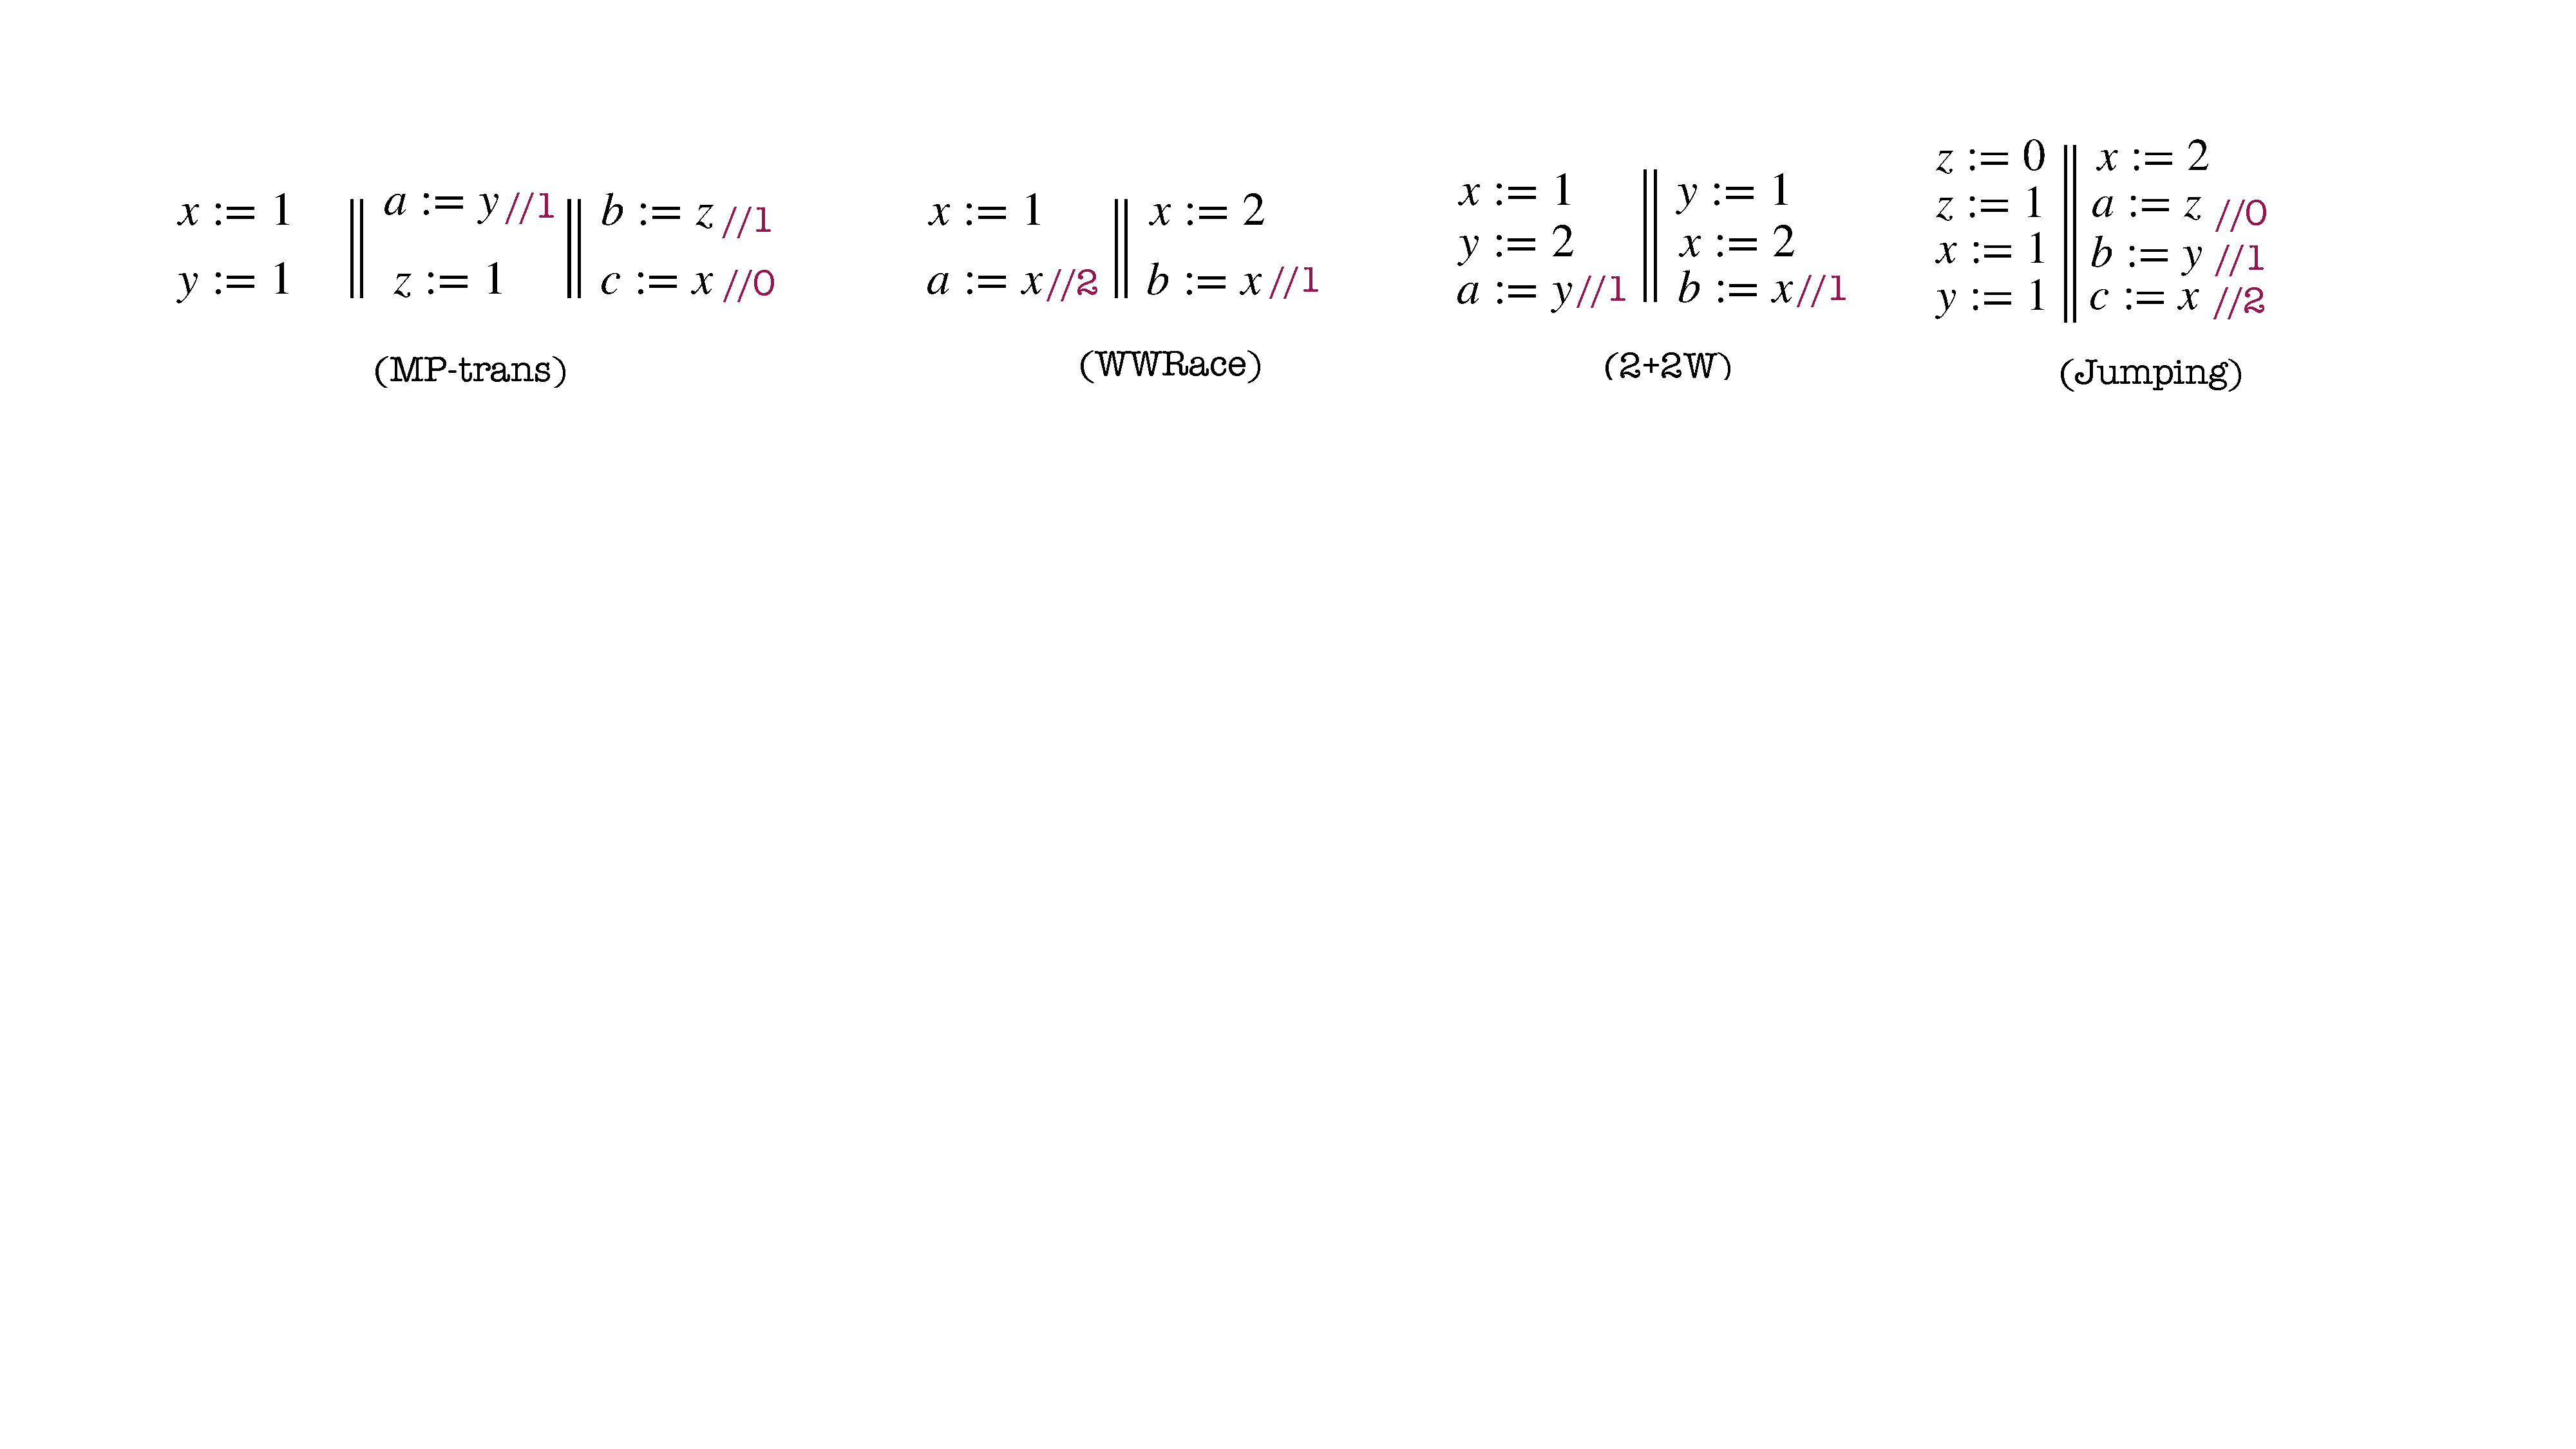
\includegraphics[width=\textwidth]{examples-violation.pdf}
%\vspace{.5cm}
\def\ystep{0.4}
 \begin{tikzpicture}[yscale=1.2]
 \begin{scope}[scale=.9]
  
 

    \node (t11) at (0,0*\ystep)  {\textcolor{green!30!blue}{$\wt(x,0)$}};
      \node (t12) at (1.5,0*\ystep) {\textcolor{green!30!blue}{$\wt(y,0)$}};
\node (t13) at (3.3,0*\ystep) {\textcolor{green!30!blue}{$\wt(z,0)$}};
    
    
    \node (t21) at (-.2,-4*\ystep)  {$\wt(x,1)$};
      \node (t22) at (1.5,-4*\ystep) {$\rd(y,1)$};
\node (t23) at (3.5,-4*\ystep) {$\rd(z,1)$};
    
   
   \node (t31) at (-.2,-8*\ystep)  {$\wt(y,1)$};
      \node (t32) at (1.5,-8*\ystep) {$\wt(z,1)$};
\node (t33) at (3.5,-8*\ystep) {$\rd(x,0)$};
\node (t34) at (2,-9.3*\ystep) {$(a)$};
    
    

  \draw[po] (t11) to (t21);
  
  \draw[po] (t12) to (t22);
  
\draw[po] (t13) to (t23);


  \draw[po] (t21) to (t31);
  
  \draw[po] (t22) to (t32);
  
\draw[po] (t23) to (t33);


  \draw[rf,bend right=-10] (t11) to node[above,pos=.5, sloped]{$\rf$} (t33);
  
  \draw[rf,bend right=20] (t32) to node[above,pos=0.8, sloped]{$\rf$} (t23);
  
  \draw[rf,bend right=20] (t31) to node[above,pos=0.8, sloped]{$\rf$} (t22);
  
%%%%%%%%%%%%%%%%%%%%%%%%%%%%%%%%%%%%%%%%%%%%%%%%%%%%%%%%%%%%%%%%%%%%%%%%%%%%%%%%%%%%%%%
%\node (t11) at (6.5,0*\ystep)  {$\wt(x,0)$};
     
    
    \node (t21) at (5.5,-4*\ystep)  {$\wt(x,1)$};
      \node (t22) at (5.5,-8*\ystep) {$\rd(x,2)$};
      
\node (t31) at (7.5,-4*\ystep)  {$\wt(x,2)$};
      \node (t32) at (7.5,-8*\ystep) {$\rd(x,1)$};

 %\draw[po] (t11) to (t21);
%\draw[po] (t11) to (t31);


  \draw[rf,bend right=0] (t31) to node[above,pos=.7, sloped]{$\rf$} (t22);
\draw[rf,bend right=0] (t21) to node[above,pos=.7, sloped]{$\rf$} (t32);

  \draw[mo,bend right=-30] (t21) to node[above,pos=.5, sloped]{$\mo$} (t31);
\draw[mo,bend right=-20] (t31) to node[below,pos=.5, sloped]{$\mo$} (t21);

\node (t33) at (6.5,-9.3*\ystep) {$(b)$};
 \draw[po] (t21) to (t22);
  
  \draw[po] (t31) to (t32);
 
%%%%%%%%%%%%%%%%%%%%%%%%%%%%%%%%%%%%%%%%%%%%%%%%%%%%%%%%%%%%%%%%%%%%%%%%%%%%%%%%%%%%%    
%\node (t11) at (9.5,0*\ystep)  {\textcolor{green!30!blue}{$\wt(x,0)$}};
%\node (t12) at (11.5,0*\ystep)  {\textcolor{green!30!blue}{$\wt(y,0)$}};
     
    \node (t21) at (9.5,-2.5*\ystep)  {$\wt(x,1)$};
      \node (t22) at (9.5,-5*\ystep) {$\wt(y,2)$};
            \node (t23) at (9.5,-7.5*\ystep) {$\rd(y,1)$};


    \node (t31) at (11.5,-2.5*\ystep)  {$\wt(y,1)$};
      \node (t32) at (11.5,-5*\ystep) {$\wt(x,2)$};
            \node (t33) at (11.5,-7.5*\ystep) {$\rd(x,1)$};
\node (t34) at (10.5,-9.3*\ystep) {$(c)$};

% \draw[po] (t11) to (t21);
\draw[po] (t21) to (t22);
\draw[po] (t22) to (t23);

% \draw[po] (t12) to (t31);
\draw[po] (t31) to (t32);
\draw[po] (t32) to (t33);
     
     
  \draw[rf,bend right=0] (t31) to node[above,pos=.9, sloped]{$\rf$} (t23);
\draw[rf,bend right=0] (t21) to node[below,pos=.7, sloped]{$\rf$} (t33);

  \draw[mo,bend right=0] (t22) to (t31);
\draw[mo,bend right=0] (t32) to node[above,pos=.5]{$\mo$} (t21);
%%%%%%%%%%%%%%%%%%%%%%%%%%%%%%%%%%%%%%%%%%%%%%%%%%%%%%%%%%%%%%%%%%%%%%%%%%%%%%%%%%%%%%

    \node (t20) at (13.5,0*\ystep)  {$\wt(z,0)$};

     
    \node (t21) at (13.5,-2.5*\ystep)  {$\wt(z,1)$};
      \node (t22) at (13.5,-5*\ystep) {$\wt(x,1)$};
            \node (t23) at (13.5,-7.5*\ystep) {$\wt(y,1)$};

    \node (t30) at (15.5,0*\ystep)  {$\wt(x,2)$};
    \node (t31) at (15.5,-2.5*\ystep)  {$\rd(z,0)$};
      \node (t32) at (15.5,-5*\ystep) {$\rd(y,1)$};
            \node (t33) at (15.5,-7.5*\ystep) {$\rd(x,2)$};
\node (t34) at (14.5,-9.3*\ystep) {$(d)$};

\draw[po] (t20) to (t21);
\draw[po] (t21) to (t22);
\draw[po] (t22) to (t23);

 \draw[po] (t30) to (t31);
\draw[po] (t31) to (t32);
\draw[po] (t32) to (t33);
     
     
  \draw[rf,bend right=0] (t20) to node[above,pos=.9, sloped]{$\rf$} (t31);
\draw[rf,bend right=0] (t23) to node[above,pos=.7, sloped]{$\rf$} (t32);
\draw[rf,bend right=-40] (t30) to node[below,pos=.7, sloped]{$\rf$} (t33);
    

  \draw[fr,bend right=-10] (t31) to node[above,pos=.5]{$\fr$}(t21);
  \draw[fr,bend right=-10] (t33) to node[below,pos=.5]{$\fr$}(t22);
  
\draw[mo,bend left=-40] (t20) to node[left,pos=.7]{$\mo$} (t21);
\draw[mo,bend left=10] (t30) to node[below,pos=.7]{$\mo$} (t22);
\end{scope}
\vspace{-\baselineskip}

   \end{tikzpicture}
\caption{\footnotesize(a) execution graph of MP-trans violating $\wramm$ : we have  $\wt(x,0)~\hb~\wt(x,1)~\hb~\rd(x,0)~\rf^{-1}~\wt(x,0)$ which violates weak-read-coherence. (b) execution graph of WWrace consistent with $\wramm$ but violating $\ramm$ : we have $\rd(x,1)~\rf^{-1}\wt(x,1)~\mo~\wt(x,2)~\hb~\rd(x,1)$ violating read coherence. (c) execution graph of 2+2W which is $\ramm$ consistent but violating 
$\sramm$ : we have $\wt(x,1)~\hb~\wt(y,2)~\mo~\wt(y,1)~\hb~\wt(x,2)~\mo~\wt(x,1)$ violating strong-write-coherence. (d) 
execution graph of Jumping which is $\sramm$ consistent, but violates $\scmm$: we have $\wt(x,1)~\po~\wt(y,1)~\rf~\rd(y,1)~\po~\rd(x,2)~\fr~\wt(x,1)$ violating 
$\acy(\po \cup \rf \cup \mo \cup \fr)$.
 }
\label{examplesra}
\vspace{-\baselineskip}
\end{figure*}


Here are a couple of useful lemmas describing the relationship between the three models $\ramm$, $\sramm$, $\wramm$ and $\rlxmm$.
 
\begin{lemma}\label{lem:sra-ra-wra-relationship}
Let $\ex = \tuple{\E, \po, \rf, \mo}$ be an execution graph. Then: $\ex \models \sramm$ implies $\ex \models \ramm$, and $\ex \models \ramm$ implies $\ex \models \wramm$. 
\end{lemma} 
\begin{proof}
  It is easy to see that if $\ex$ satisfies strong-write-coherence, then it satisfies write-coherence also. Hence $\ex \models \sramm$ implies $\ex \models \ramm$. For $\ramm$ to $\wramm$, we show that if weak-read-coherence is violated, then either read-coherence or write-coherence is violated: suppose weak-read-coherence is violated, there is a cycle $\rd(x) \xra{\rf^{-1}} \wt_1(x) \xra{\hb} \wt_2(x) \xra{\hb} \rd(x)$. The $\mo$ relation can order $\wt_1$ and $\wt_2$ in either way. If $\wt_1(x) \xra{\mo} \wt_2(x)$, then read-coherence is violated, and if $\wt_2(x) \xra{\mo} \wt_2(x)$, then write-coherence is violated.
\end{proof}

\begin{lemma}\label{lem:sra-ra-rlx-relationship}
Let $\ex = \tuple{\E, \po, \rf, \mo}$ be an execution graph. Then: $\ex \models \ramm$ implies $\ex \models \rlxmm$, and $\ex \models \ramm$ implies $\ex \models \rlxmm$. 
\end{lemma}

\begin{proof}

If $\ex$ satisfies \WCoh{}, then it satisfies \RlxWCoh. Similarly, if $\ex$ satisfies \RCoh{}, then $\ex$ also satisfies \RlxRCoh{}. This is because in both cases $\hb$ is replaced by $\po$ in the coherence axioms. Hence $\ex \models \ramm$ implies $\ex \models \rlxmm$.

\end{proof}

 
\begin{figure*}[h]
%  \vspace{-\baselineskip}
%\vspace{.5cm}
\begin{center}
 

\def\ystep{0.4}
 \begin{tikzpicture}[yscale=1.2]
 \begin{scope}[scale=1]
 %wra
    \node (t21) at (0,0*\ystep)  {$\wt(x,1)$};
      \node (t22) at (0,-3*\ystep) {$\rd(x,2)$};
     \node (t31) at (2,0*\ystep) {$\wt(x,2)$};
     \node (t32) at (2,-3*\ystep) {$\rd(x,1)$};

\node (t34) at (1,-4*\ystep) {$(a)$};

% \draw[po] (t11) to (t21);
\draw[po] (t21) to (t22);
\draw[po] (t31) to (t32);
 
     
  \draw[rf,bend right=0] (t21) to node[above,pos=.9, sloped]{$\rf$} (t32);
\draw[rf,bend right=0] (t31) to node[below,pos=.7, sloped]{$\rf$} (t22);

  \draw[mo,bend right=5] (t21) to (t31);
\draw[mo,bend right=5] (t31) to node[above,pos=.5]{$\mo$} (t21);
%%%%%%%%%%%%%%%%%%%%%%%%%%%%%%%%%%%%%%%%%%%%%%%%%%%%%%%%%%%%%%%%%%%%%%%%%%%%%%%%%%%%%%

%%rlx
\node (t21) at (6,0*\ystep)  {$\wt(x,1)$};
      \node (t22) at (6,-3*\ystep) {$\wt(x,2)$};
      \node (t23) at (6,-6*\ystep) {$\wt(y,1)$};
      
     \node (t31) at (8,0*\ystep) {$\rd(y,1)$};
     \node (t32) at (8,-6*\ystep) {$\rd(x,1)$};

\node (t34) at (7,-7*\ystep) {$(b)$};

% \draw[po] (t11) to (t21);
\draw[po] (t21) to (t22);
\draw[po] (t22) to (t23);
\draw[po] (t31) to (t32);
 
     
  \draw[rf,bend right=0] (t23) to node[above,pos=.7, sloped]{$\rf$} (t31);
\draw[rf,bend right=0] (t21) to node[below,pos=.7, sloped]{$\rf$} (t32);
 \end{scope}
\vspace{-\baselineskip}


   \end{tikzpicture}
   \end{center}
\caption{\footnotesize (a) $\wramm$-consitent but violates \RlxRCoh{} and hence not $\rlxmm$-consistent.
 (b) $\rlxmm$-consitent but violates \WRCoh{} and hence not $\wramm$-consistent.
 }\label{example-rlxwra}
\vspace{-\baselineskip}
\end{figure*}
\paragraph*{Comparing memory models.} The two lemmas gives the following partial order of the memory models reflecting the number of allowed behaviours: $\scmm\preccurlyeq\sramm\preccurlyeq\ramm\preccurlyeq\{\wramm,\rlxmm\}$ with models towards the right allowing more behaviors.  All models are weaker than $\scmm$. $\rlxmm$ is weaker than $\ramm$ but incomparable with $\wramm$. In particular, the lack of synchronization across $\rf$
in $\rlxmm$ makes $\hb$ weaker in $\rlxmm$ compared to $\wramm$. On the other hand, $\wramm$ allows extra behaviors over $\rlxmm$ because it does not enforce \WRCoh{}. Figure~\ref{example-rlxwra} shows examples to demonstrate the incomparability between $\wramm$ and $\rlxmm$.

An execution graph $\ex = \tuple{\E, \po, \rf, \mo}$ is consistent with memory model $\MemModel$ if it satisfies all the axioms corresponding to $\MemModel$ as shown in Table  ~\ref{table:ax:models-2}. We write $\ex \models \MemModel$ if $\ex$ is consistent with $\MemModel$. For a partial execution graph $\expartial = \tuple{\E, \po}$, we write $\expartial \models \MemModel$ if there exists an $\rf$ and $\mo$ such that $\ex \models \MemModel$ for the complete execution graph $\ex = \tuple{\E, \po, \rf, \mo}$. Hence, the general consistency testing problem $\vm$ can be stated as: given a partial execution graph $\expartial$ and a memory model $\MemModel$, does $\expartial \models \MemModel$? 
Alternatively, we can frame the problem as follows.
\begin{center}
  \fbox{%
    \begin{minipage}{0.98\textwidth}
      \noindent \textsc{Verifying weak memory consistency} (The $\vm$-problem)

      \medskip

      \noindent \textbf{Instance:} A partial execution graph $\expartial=\tuple{\E, \po}$ and a memory model $\MemModel \in \{\ramm, \sramm, \wramm, \rlxmm\}$

      \medskip

      \noindent \textbf{Question:} Do there exist $\rf$ and $\mo$ relations on $\E$ such that the complete execution graph $\ex = \tuple{\E, \po, \rf, \mo}$ satisfies the consistency axioms of the memory model $\MemModel$?
    \end{minipage}%
  }
\end{center}

The next chapter shall solely deal with the above problem. We shall, as in VSC$^\pp$, classify the results based on the number of writers per variable. The next two chapters would contain relevant theorems and proofs related for $\vm$ when the model is $\ramm$. The weak and strong variants of $\ramm$ are also placed alongside in these chapters.

The following two chapters will be dedicated to results related to $\rlxmm$ memory model and even later we shall discuss similar results for  some of the causal memory models. I have not left any detailing about them here. We shall understand them as they appear.








\chapter{Verifying Release-Acquire Consistency}

The problem of consistency testing asks whether a given observed execution can be consistent with a particular memory model. The $\vm$ problem is an extension of the fundamental VSC-problem introduced by Gibbons and Korach  \cite{gibbons}. Later, Cantin et al.\cite{CantinLS05} proved that the problem remains NP-complete even with a single memory
location (but with unboundedly many threads) which also implies NP-completness for all memory
models that adhere to the “SC-per-location” property, such as  RA, SRA and Relaxed.  Charkraborty et al. \cite{ChakrabortyKMP24} asked 'how hard is weak-memory testing?' when the input parameters are bounded. They showed that the complexity of consistency testing for weak memory models including $\ramm$, $\sramm$ and $\wramm$ is NP-hard even when the syntactic parameters like number of threads, variables and values are fixed. The only thing that remained unbounded were the number of events. Does this tells us that there can never be any kind of parameterization?

We now ask similar question but choose a different parameter. We choose to bound the number of threads (writers) writing to a variable. The results show that the problem remains $\NP$-hard for $\twowriter$ but becomes  polynomial for $\onewriter$.  Here is a summarization of the  hardness results for $\ramm$ and its variants.

\begin{itemize}
\item For \onewriter\ programs, we prove that there is no $\mathcal{O}(n^{\frac{3}{2} - \epsilon})$-time algorithm, under the Boolean Matrix Multiplication (BMM) hypothesis, for any $\epsilon > 0$. 
\item When we consider \twowriter\ programs (those where each variable is written into by atmost two threads), the problem continues to be $\np$-complete. 
\item Furthermore, when we consider \threewriter\ programs, the problem admits a conditional lower bound under the Exponential Time Hypothesis (ETH): there is no $2^{o(k)} \cdot n^{\mathcal{O}(1)}$ algorithm, where $k$ is the number of threads, and $n$ is the total number of operations.
\end{itemize}
The results provide a tight complexity picture while bounding the number of writer threads per memory location, with \onewriter\ giving polynomial-time, \twowriter\ being $\NP$-hard and \threewriter\ allowing a stronger conditional lower bound. 


%\begin{restatable}{theorem}{thmwracorrectness}
%A partial execution graph $\expartial = \tuple{\E, \po}$ of a one-writer system is consistent for $\ramm$, $\sramm$ and $\wramm$ iff Algorithm~\ref{algo:one-writer-wra} returns $\expartial$ is $\wramm$-consistent. Moreover, the algorithm runs in time $\mathcal{O}(n^3)$ where $n = |E|$ and returns the smallest $\rf$  that is $\wramm$-consistent, if one exists.
%\end{restatable}

%We also have the following conditional lower bound assuming the Boolean Matrix Multiplication (BMM) hypothesis which states that: There is no $\mathcal{O}(n^{3-\epsilon})$ algorithm for Boolean Matrix Multiplication, for any $\epsilon > 0$. 

%\begin{restatable}{theorem}{thmwracorrectness}
%A partial execution graph $\expartial = \tuple{\E, \po}$ of a one-writer system is consistent for $\sramm$, $\ramm$ and $\wramm$ iff  Algorithm~\ref{algo:one-writer-wra} returns $\expartial$ is $\wramm$-consistent. Moreover, the algorithm runs in time $\mathcal{O}(n^3)$ where $n = |E|$ and returns the smallest $\rf$  that is $\wramm$-consistent, if one exists.
%\end{restatable}

%For multiple writers the problem becomes NP-Complete. Infact the problem has a fine grained lower bound if the Exponential Time  Hypothesis is true.

%\begin{theorem}\label{thm:eth-hardness}
 %   Under ETH, there is no $2^{o(k)} \cdot n^{\mathcal{O}(1)}$ algorithm for the $\vm$-problem with $\MemModel \in \{ \sramm, \ramm, \wramm\}$, $k$ being the number of threads, and $n$ the number of events. The result holds even while restricting the input instance to \threewriter\ execution graphs.
%\end{theorem}

%\begin{theorem}
%\label{thm:two-writer-hardness}
   % The $\vm$ problem is $\NP$-complete for $\MemModel \in \{\sramm, \ramm, \wramm\}$, even when restricted to \twowriter\ execution graphs.
%\end{theorem}

 This chapter will only have theorems and proofs for $\onewriter$ programs. The other results will be reflected in the next chapter. 
 
\section{Polynomial-time algorithm for \onewriter\ systems}
\label{sec:onewriter}

We now consider programs where, for every variable, there is a single thread which writes to it. Any number of threads can read from a variable. An execution graph $\ex = \tuple{\E, \po, \rf, \mo}$ is said to be a \onewriter\ execution graph if for each memory location $x$, the entire set of its write events $\W_x$ belong to one thread. 

\noindent \textbf{Overview of this section.} The fact that we work with \onewriter\ execution graphs simplifies several axioms of Table~\ref{table:ax:models-2}, allowing for  a polynomial-time procedure. Recall however that for sequential consistency, the \onewriter\ assumption offers no specific advantage and still yields a $\NP$-hard complexity~\cite{gibbons}. 

\noindent \textit{$\sramm$ and $\ramm$ reduce to $\wramm$.} Firstly, we note that consistency checking for the $\sramm$ and $\ramm$ memory models reduce to checking for $\wramm$ in \onewriter\ execution graphs (Lemma~\ref{lem:one-writer-reduces-to-wra}). Moreover, since all writes of a memory location lie in a single thread, the $\mo$ relation on writes gets fixed to the unique order that agrees with $\po$.  Therefore, the problem boils down to detecting if there is an $\rf$ that satisfies \emph{porf-acyclicity} and \emph{weak-read-coherence}, the two axioms needed for $\wramm$ consistency. So we focus on these two axioms for the rest of the section. 

\noindent \textit{A partial order on $\rf$.} Secondly, since all writes to a memory location $x$ are totally ordered by $\po$, there is a natural partial order induced on the $\rf$ relations. A reads-from relation $\rf_1$ is said to be smaller than $\rf_2$, written as $\rf_1 \sqsubseteq \rf_2$, if for every 
read $r$, the write event $w_2 = \rf^{-1}_2(r)$ appears $\po$-later than $w_1 = \rf^{-1}_1(r)$ (we say $w_2$ is $\po$-later than $w_1$ if $w_1~\po^*w_2$). In other words, $\rf_2$ associates each read $r$ to a write that appears later in the program order compared to the write that $\rf_1$ associates it to\label{order}. %%%%%%% 
We observe two useful properties of this partial order: (1) if an $\rf$ violates porf-acyclicity, then every $\rf^{\dagger}$ larger than it also violates porf-acyclicity, and (2) among all the $\rf$ that satisfy weak-read-coherence, there is a unique minimum element $\rf_{\min}$.

\noindent \textit{Algorithm.} Using these two properties, we design an algorithm that starts with the smallest $\rf$ and iteratively computes larger reads-from relations until a $\wramm$-consistent $\rf$ is found. If this $\rf$ additionally satisfies porf-acyclicity, we have found a reads-from relation that witnesses the $\wramm$-consistency. Else, we conclude that no such $\rf$ exists.  

The two useful properties appear in Section~\ref{sec:onewriter-structural-properties} and the algorithm is described in Section~\ref{sec:onewriter-algorithm}. Section~\ref{sec:1-writer-hardness} presents a lower bound for \onewriter\ systems.

\subsection{Structural properties of \onewriter\ execution graphs}
\label{sec:onewriter-structural-properties}
Our first observation is that for \onewriter\ systems, checking $\sramm$ and $\ramm$ reduces to checking $\wramm$.  For $\wramm$ the only axioms are porf-acyclicity and weak-read-coherence.  For $\ramm$ one must also ensure write-coherence and read-coherence, in addition to porf-acyclicity.  In a \onewriter\ setting, write-coherence is enforced by choosing $\mo$ to agree with $\po$ (so all writes to a location are ordered by the program order of their single writer).  

A violating cycle for read-coherence has the form
\[
\rd(x) \xra{\rf^{-1}} \wt(x) \xra{\mo_x} \wt'(x) \xra{\hb} \rd(x).
\]
When $\mo$ agrees with $\po$, the $\mo_x$ edge is simply $\po^+$, since both $\wt_x$ and $\wt'_x$ are in the same thread. Now, a violating cycle for weak-read-coherence has the form
\[
\rd(x) \xra{\rf^{-1}} \wt(x) \xra{\hb} \wt'(x) \xra{\hb} \rd(x),
\]
and, since $\wt(x)$ and $\wt'(x)$ come from the same thread, the $\hb$ step between $\wt(x)$ and $\wt'(x)$ can likewise be instantiated by $\po^+$.  Hence read-coherence coincides with weak-read-coherence in the \onewriter\ setting.  Moreover, having an $\mo$ agreeing with $\po$ reduces strong-write-coherence to porf-acyclicity, culminating in this lemma.  

\begin{restatable}{lemma}{lemonewriterreducestowra}
    \label{lem:one-writer-reduces-to-wra}
 Let $\ex = \tuple{\E, \po, \rf, \mo}$ be a \onewriter\ execution graph. Then, for $\MemModel \in \{\sramm, \ramm\}$, we have $\ex \models \MemModel$ iff $\mo$ agrees with $\po$ and $\ex \models \wramm$. 
\end{restatable}
\begin{proof}
    Let us begin with $\MemModel = \ramm$. For $\ex$ to be consistent with $\ramm$, it has to satisfy the three axioms: porf-acyclicity, write-coherence and read-coherence~(see Table~\ref{table:ax:models-2}). In a \onewriter\ system, for $\mo$ edges, both its source and target are in the same thread. Therefore, to satisfy write-coherence, $\mo$ should agree with $\po$: in other words, if $w_1~\mo_x~w_2$, then $w_1~\po^+~w_2$. Hence, notice that to prove the lemma, it is sufficient to show that the read-coherence axiom and weak-read-coherence axiom coincide for \onewriter. A violating cycle for read-coherence is of the form
    \[r \xra{\rf} w_1 \xra{\mo_x} w_2 \xra{\hb} r\]
    As seen above the $\mo_x$ edge is simply $\po^+$, hence $w_1 \xra{\mo_x} w_2$ can be replaced with $w_1 \xra{\po^+} w_2$. A violating cycle for weak-read-coherence is of the form
    \[r \xra{\rf} w_1 \xra{\hb} w_2 \xra{\hb} r\]
    with $w_1$ and $w_2$ being writes on the same variable $x$. Since the writes are on the same variable, $w_1 \xra{\hb} w_2$ can be replaced with $w_1 \xra{\po^+} w_2$. This proves that the violating cycles for both the axioms coincide for \onewriter\ systems.

    Now, let $\MemModel = \sramm$. For strong-write-coherence to be true, we require $\mo$ to agree with $\po$. If $X \models \sramm$, then the axioms porf-acyclicity, strong-write-coherence and read-coherence are true. Since strong-write-coherence holds, $\mo$ needs to agree with $\po$. We have shown above that read-coherence coincides with weak-read-coherence, when $\mo$ agrees with $\po$. Hence $X \models \wramm$. Now, for the other direction. Suppose $\mo$ agrees with $\po$ and weak-read-coherence are true. From above, we deduce read-coherence holds. If strong-write-coherence is violated, then there will be a porf-cycle, a contradiction. Hence, the lemma follows for $\MemModel = \sramm$.
\end{proof}
As a consequence, the consistency checking of \onewriter\ under $\sramm$, $\ramm$ and $\wramm$ boils down to checking porf-acyclicity and weak-read-coherence violations.
Secondly, the problem of synthesizing both $\rf$ and $\mo$ boils down to just synthesizing $\rf$, since $\mo$ is fixed to the order that respects $\po$. Nevertheless, there are still exponentially many $\rf$ relations possible. The next lemma entails that there is a ``smallest'' $\rf$ among all $\wramm$-consistent $\rf$s in the $\sqsubseteq$ order on $\rf$s defined in the overview of this section. Given $\rf_1, \rf_2$, we write $\min(\rf_1, \rf_2)$ for the reads-from relation which associates every read $r$ to the $\po$-smaller write between $\rf^{-1}_1(r)$ and $\rf^{-1}_2(r)$.


\begin{restatable}{lemma}{lemmaonewritertwoproperties}
    \label{lem:onewriter-axioms-two-properties}
Let $\rf_1$ and $\rf_2$ be two reads-from relations over a partial \onewriter\ execution graph $\ex=\tuple{\E, \po, \mo}$ s.t. $\mo$ agrees with $\po$. 
\begin{itemize}
\item Suppose $\rf_1 \sqsubseteq \rf_2$. Then, if $\rf_1$ induces a $\po \cup \rf_1$ cycle, then $\rf_2$ induces a $\po \cup \rf_2$ cycle.
\item Suppose both $\rf_1$ and $\rf_2$ satisfy weak-read-coherence. Then,  $\min(\rf_1, \rf_2)$ also satisfies weak-read-coherence.
\end{itemize} 
\end{restatable}
\begin{proof}
For the first item, suppose $\rf_1$ induces a porf-cycle of the form:
\[ e_1 \xra{\rf_1} f_1 \xra{\po} e_2 \xra{\rf_1} f_2 \cdots e_m \xra{\rf_1} f_{m} \xra{\po} e_1\]
Notice that each $e_i$ is a write event and $f_i$ is a read event such that $e_i = \rf_1(f_i)$. Since $\rf_1 \sqsubset \rf_2$, we know $\rf_1(f_i) \xra{\po^*} \rf_2(f_i)$. Hence: $e_i \xra{\po^*} e'_i$ where $e'_i = \rf_2(f_i)$. This gives the following $\po \cup \rf_2$ cycle:
 \[ e_1 \xra{\po^*} e'_1 \xra{\rf_2} f_1 \xra{\po} e_2 \xra{\po^*} e'_2 \xra{\rf_2} f_2 \cdots e_m \xra{\po^*} e'_m \xra{\rf_2} f_{m} \xra{\po} e_1\]
 This proves the first item.

 For the second item, denote $\rf_0 = \min(\rf_1, \rf_2)$. We will show that if $\rf_0$ violates weak-read-coherence, then either $\rf_1$ or $\rf_2$ violates it. Suppose $\rf_0$ induces a violation of weak-read-coherence. There is a cycle of the form:
 \[ r \xra{\rf_0^{-1}} w \xra{\po^+} w' \xra{\hb_0} r \]
 where both $w$ and $w'$ are on the same variable, and hence the edge between them is $\po^+$. By definition, either $\rf_1$ or $\rf_2$ associates $r$ to $w$. Let us say $\rf_1(r) = w$. If we show $w' \hb_0 r$ then we are done. Since $w'~\hb_0~r$, there is a path with $\po$ and $\rf_0$ edges from $w'$ to $r$:
 \[w' \xra{\po^*} e_1 \xra{\rf_0} f_1 \xra{\po^*} e_2 \xra{\rf_0} f_2 \cdots e_m \xra{\rf_0} f_m \xra{\po^*} r \]
 We will now form a $\po \cup \rf_1$ path from $w'$ to $r$. For each $e_i \xra{\rf_0} f_i$, either $e_i \xra{\rf_1} f_i$ too, in which case we retain that edge. If not, by construction of $\rf_0$, we know that $e_i \xra{\rf_2} f_i$ and $e_i \po^* \rf_1(f_i)$. Replace $e_i \xra{\rf_0} f_i$ by the sequene $e_i \po^* \rf_1(f_i) \xra{\rf_1} f_i$ as in the proof of the first item, to deduce an $\hb_1$ path from $w'$ to $r$. This show that there is a violating cycle for weak-read-coherence induced by $\rf_1$ too, thereby proving the second item. 
\end{proof}
Suppose $S$ is the set of all $\rf$ that satisfy weak-read-coherence. The second item of Lemma~\ref{lem:onewriter-axioms-two-properties} implies that $S$ contains a unique minimum element, which we denote by $\rf_{\min}$. By the first item of Lemma~\ref{lem:onewriter-axioms-two-properties}, if $\rf_{\min}$ violates porf-acyclicity then every $\rf$ in $S$ also violates it. Therefore, $\wramm$-consistency checking reduces to computing $\rf_{\min}$ and testing it for porf-acyclicity. The algorithm in the next section performs exactly this construction and test. 

\begin{figure}[!tbp]
   \def\ystep{0.5}

\centering
	\scalebox{.7}{
\begin{tikzpicture}[yscale=1]
\node (t01) at (-.2, 1.5*\ystep) {$t_1$};
\node (t02) at (1.5, 1.5*\ystep) {$t_2$};
\node (t03) at (3, 1.5*\ystep) {$t_3$};

  \node (t11) at (-.2, 0*\ystep) {$\wt_1(x,1)$};
    \node (t12) at (1.5, 0*\ystep) {$\rd_1(x,2)$};
    \node (t13) at (3, 0*\ystep) {$\rd_2(y,1)$};
    
    
    \node (t21) at (-.2, -2*\ystep) {$\wt_2(x,2)$};
    \node (t22) at (1.5, -2*\ystep) {$\rd_3(x,1)$};    
    
    \node (t23) at (3, -2*\ystep) {$\rd_4(x,2)$};
    
    
    \node (t31) at (-.2, -4*\ystep) {$\wt_3(x,1)$};
    \node (t32) at (1.5, -4*\ystep) {$\wt_4(y,1)$};
    
    \node (t41) at (-.2, -6*\ystep) {$\wt_5(x,2)$};
    
    \node (n1) at (1.5,-8*\ystep) {$\rf_0$};
    
    \draw[po] (t11) -- (t21);
    \draw[po] (t21) -- (t31);
    \draw[po] (t31) -- (t41);
    
    \draw[po] (t12) -- (t22);
    \draw[po] (t22) -- (t32);
    \draw[po] (t13) -- (t23);
    
      
    \draw[rf] (t11) -- (t22);
    \draw[rf] (t21) -- (t12);
    \draw[rf] (t21) to[out=-25,in=-160] (t23);
    \draw[rf] (t32) -- (t13);
    
    %%%%rf_0%%%%
    \node (t01) at (5, 1.5*\ystep) {$t_1$};
\node (t02) at (6.5, 1.5*\ystep) {$t_2$};
\node (t03) at (8, 1.5*\ystep) {$t_3$};

  \node (t11) at (5, 0*\ystep) {$\wt_1(x,1)$};
    \node (t12) at (6.5, 0*\ystep) {$\rd_1(x,2)$};
    \node (t13) at (8, 0*\ystep) {$\rd_2(y,1)$};
    
    
    \node (t21) at (5, -2*\ystep) {$\wt_2(x,2)$};
    \node (t22) at (6.5, -2*\ystep) {$\rd_3(x,1)$};   
    \node (t23) at (8, -2*\ystep) {$\rd_4(x,2)$};
    
    
    \node (t31) at (5, -4*\ystep) {$\wt_3(x,1)$};
    \node (t32) at (6.5, -4*\ystep) {$\wt_4(y,1)$};
    
    \node (t41) at (5, -6*\ystep) {$\wt_5(x,2)$};
    
    \node (n1) at (6.5,-8*\ystep) {$\rf_1$};
    
    \draw[po] (t11) -- (t21);
    \draw[po] (t21) -- (t31);
    \draw[po] (t31) -- (t41);
    
    \draw[po] (t12) -- (t22);
    \draw[po] (t22) -- (t32);
    \draw[po] (t13) -- (t23);
    
      
    \draw[rf] (t31) -- (t22);
    \draw[rf] (t21) -- (t12);
    \draw[rf] (t21) to[out=-25,in=-160] (t23);
    \draw[rf] (t32) -- (t13);
    
    %%%%rf_1%%%%
    
    \node (t01) at (10, 1.5*\ystep) {$t_1$};
\node (t02) at (11.5, 1.5*\ystep) {$t_2$};
\node (t03) at (13, 1.5*\ystep) {$t_3$};

  \node (t11) at (10, 0*\ystep) {$\wt_1(x,1)$};
    \node (t12) at (11.5, 0*\ystep) {$\rd_1(x,2)$};
    \node (t13) at (13, 0*\ystep) {$\rd_2(y,1)$};
    
    
    \node (t21) at (10, -2*\ystep) {$\wt_2(x,2)$};
    \node (t22) at (11.5, -2*\ystep) {$\rd_3(x,1)$};   
    \node (t23) at (13, -2*\ystep) {$\rd_4(x,2)$};
    
    
    \node (t31) at (10, -4*\ystep) {$\wt_3(x,1)$};
    \node (t32) at (11.5, -4*\ystep) {$\wt_4(y,1)$};
    
    \node (t41) at (10, -6*\ystep) {$\wt_5(x,2)$};
    
    \node (n1) at (11.5,-8*\ystep) {$\rf_2$};
    
    \draw[po] (t11) -- (t21);
    \draw[po] (t21) -- (t31);
    \draw[po] (t31) -- (t41);
    
    \draw[po] (t12) -- (t22);
    \draw[po] (t22) -- (t32);
    \draw[po] (t13) -- (t23);
    
      
    \draw[rf] (t31) -- (t22);
    \draw[rf] (t21) -- (t12);
    \draw[rf] (t41) to[out=-15,in=250] (t23);
    \draw[rf] (t32) -- (t13);

     \end{tikzpicture}}
     


\caption{\footnotesize From left: $\rf_0 \sqsubseteq \rf_1 \sqsubseteq \rf_2$. $\rf_0$ has a violation of \WRCoh{}:~$\rd_3 \xra{\rf_{0}^{-1}} \wt_1 \xra{\po} \wt_2 \xra{\hb_0} \rd_3 $.  $\rf_1$ has a violation of \WRCoh{}:~$\rd_4 \xra{\rf_{1}^{-1}} \wt_2 \xra{\po} \wt_3 \xra{\hb_1} \rd_4 $. $\rf_2$ does not have any more violations of \WRCoh{}. \PORF{} is also satisfied by $\rf_2$. The underlying partial execution graph is $\wramm$-consistent.
}\label{Example-one-writer-without-porfcycle}

\end{figure}

\subsection{Algorithm}
\label{sec:onewriter-algorithm}

Our algorithm starts from an $\rf_0$ which maps every read $r$ to the $\po$-smallest  write in its writer thread, such that the value of the chosen write matches with that of $r$, and in case the writer thread is the same as the one where $r$ is present, the mapped write lies above $r$. This relation $\rf_0$ may not satisfy weak-read-coherence. In that case, a violating cycle is identified and $\rf_0$ is modified to $\rf_1$ as explained below. Assume we have iteratively constructed upto $\rf_i$, and $\rf_i$ does not satisfy weak-read-coherence.  



%\begin{wrapfigure}[20]{r}{0.4\textwidth}
   
\begin{figure} 
  \def\ystep{0.5}
\centering
	\scalebox{.7}{
\begin{tikzpicture}[yscale=1]
\node (t01) at (-.2, 1.5*\ystep) {$t_1$};
\node (t02) at (1.5, 1.5*\ystep) {$t_2$};

  \node (t11) at (-.2, 0*\ystep) {$\wt_1(x,1)$};
    \node (t12) at (1.5, 0*\ystep) {$\rd_1(x,2)$};
    
    \node (t21) at (-.2, -2*\ystep) {$\wt_2(x,2)$};
    \node (t22) at (1.5, -2*\ystep) {$\rd_3(x,1)$};    
    
    \node (t31) at (-.2, -4*\ystep) {$\rd_2(y,1)$};
    \node (t32) at (1.5, -4*\ystep) {$\wt_4(y,1)$};
    
    \node (t41) at (-.2, -6*\ystep) {$\wt_5(x,1)$};
    
    \node (n1) at (1.1,-8*\ystep) {$\rf_0$};
    
    \draw[po] (t11) -- (t21);
    \draw[po] (t21) -- (t31);
    \draw[po] (t31) -- (t41);
    
    \draw[po] (t12) -- (t22);
    \draw[po] (t22) -- (t32);
      
    \draw[rf] (t21) to (t12);
    \draw[rf] (t11) -- (t22);
    \draw[rf] (t32) to (t31);
    \node (t01) at (4, 1.5*\ystep) {$t_1$};
\node (t02) at (5.5, 1.5*\ystep) {$t_2$};

  \node (t11) at (4, 0*\ystep) {$\wt_1(x,1)$};
    \node (t12) at (5.5, 0*\ystep) {$\rd_1(x,2)$};
    
    \node (t21) at (4, -2*\ystep) {$\wt_2(x,2)$};
    \node (t22) at (5.5, -2*\ystep) {$\rd_3(x,1)$};   
    
    \node (t31) at (4, -4*\ystep) {$\rd_2(y,1)$};
    \node (t32) at (5.5, -4*\ystep) {$\wt_4(y,1)$};
    
    \node (t41) at (4, -6*\ystep) {$\wt_5(x,1)$};
    
    \node (n1) at (5.2,-8*\ystep) {$\rf_1$};
    
     \draw[po] (t11) -- (t21);
    \draw[po] (t21) -- (t31);
    \draw[po] (t31) -- (t41);
    
    \draw[po] (t12) -- (t22);
    \draw[po] (t22) -- (t32);
    
    \draw[rf] (t21) to (t12);
    \draw[rf] (t41) to[out=30,in=-135] (t22);
    \draw[rf] (t32) to (t31);
    
    \end{tikzpicture}}
     


\caption{\footnotesize From left: $\rf_0 \sqsubseteq \rf_1$. $\rf_0$ has a violation of \WRCoh{}:~$\rd_3 \xra{\rf_{0}^{-1}} \wt_1 \xra{\po} \wt_2 \xra{\hb} \rd_3 $.  $\rf_1$ has no \WRCoh{} violation but does not satisfy \PORF{}:~$\wt_5 \xra{\rf_{1}} \rd_3 \xra{\po} \wt_4 \xra{\rf} \rd_2 \xra{\po} \wt_5$. The partial execution graph is not $\wramm$-consistent.
}\label{Example-one-writer-with-porfcycle}  
\end{figure}

\noindent \emph{From $\rf_i$ to $\rf_{i+1}$.} Pick a violating cycle for weak-read-coherence:
\[ r_i \xra{\rf_{i}^{-1}} w_i \xra{\hb_i} w'_i \xra{\hb_i} r_i \]
where all three events $r_i, w_i, w'_i$ are over the same variable, say $x_i$, and $\hb_i$ is $(\po \cup \rf_i)^+$. Recall that since we are in the \onewriter\ case, the intermediate $\hb_i$ can be replaced with $\po^+$. Modify $\rf_i$ to eliminate the violating cycle: choose a write for $r_i$ which appears on or after $w'_i$, that is, pick $w''_i$ such that $w'_i~\po^* w''_i$ and $w''_i$ is a write on the same variable $x_i$, writing the same value as the read event $r_i$. If no such write exists, conclude that there is no $\rf$ for $\expartial$ that satisfies weak-read-coherence. Else, let the resulting $\rf$ be called $\rf_{i+1}$. If $\rf_{i+1}$ does not satisfy weak-read-coherence, we update $\rf_{i+1}$ as above. Else, $\rf_{i+1}$ satisfies weak-read-coherence. We declare $\rf_{\min} = \rf_{i+1}$.

Finally, we test whether $\rf_{\min}$ satisfies porf-acyclicity. If it does, we have a witness for $\wramm$-consistency. Else, we conclude (due to Lemma~\ref{lem:onewriter-axioms-two-properties}) that $\expartial$ is not $\wramm$-consistent. 
We formalize this discussion in Algorithm~\ref{algo:one-writer-wra}. Here is the key invariant maintained by the algorithm: at each step $i$ where the update function is called on $\rf_i$,  we can show that $\rf_i \sqsubseteq \rf^{\dagger}$ for every $\rf^\dagger$ that satisfies weak-read-coherence. Figures~\ref{Example-one-writer-without-porfcycle} and ~\ref{Example-one-writer-with-porfcycle} illustrate the running of the algorithm on two different partial execution graphs. 





\begin{algorithm}[h!]
\caption{$\wramm$-consistency checking in \onewriter\ systems}
\label{algo:one-writer-wra}
\Fn{$\CheckC(\expartial)$}{
    $\rf \gets \Initialize(\expartial)$ \\
    \While{$\rf$ violates weak-read-coherence}{\label{algo-while-main-onewriter}
        $\rf \gets \update(\expartial, \rf)$  \label{algo-update-call}
    }
    \Comment{Now $\rf = \rf_{\min}$}
    \If{$\rf$ satisfies porf-acyclicity}{ \label{algo-check-porf}
        \Return $\expartial$ is $\wramm$-consistent \label{algo-declare-consistent}
    }
    \Else {
        \Return $\expartial$ is not $\wramm$-consistent  \label{algo-porf-cycle}
    }
}


\Fn{$\Initialize(\expartial)$}{
\For{each read $r = \rd(x, v)$}{
$t \gets$  thread containing $r$ \\
$t_x \gets$ writer thread for $x$ \\
\If{$t \neq t_x$}{
    $\rf^{-1}_0(r) \gets$ $\po$-smallest write $w$ of the form $\wt(x,v)$ in $t_x$ \\
    \If{there is no such write}{
        \Return $\expartial$ is not $\wramm$-consistent \label{init-not-consistent1}
    }
}
\If{$t = t_x$}{
    $\rf^{-1}_0(r) \gets$ $\po$-smallest write $w$ of the form $\wt(x,v)$ in $t_x$ s.t. $w~\po^+r$ \\
    \If{there is no such write}{
        \Return $\expartial$ is not $\wramm$-consistent \label{init-not-consistent2}
    }
}
}
\Return $\rf_0$
}

\Fn{$\update(\expartial, \rf_i)$}{
    Pick a cycle violating weak-read-coherence: $r_i \xra{\rf_i^{-1}} w_i \xra{\hb_i} w'_i \xra{\hb_i} r_i$ \label{algo-violatecycle} \\
    Let $r_i = \rd(x, v)$, $w_i = \wt(x, v)$, $w'_i = \wt(x, v')$ \\
    $t \gets$ thread of $r_i$ \\
    $t_x \gets$ writer thread of variable $x$ \\
    \If{$t \neq t_x$}{
    $\rf^{-1}_{i+1}(r_i) \gets$ $\po$-smallest write $w''_i$ of the form $\wt(x,v)$ in $t_x$ s.t. $w'_i ~\po* w''_i$ \label{algo-update1} \\
    \If{there is no such write}{
        \Return $\expartial$ is not $\wramm$-consistent  \label{algo-update-notconsistent1}
    }
}
\If{$t = t_x$}{
    $\rf^{-1}_{i+1}(r_i) \gets$ $\po$-smallest write $w''_i$ of the form $\wt(x,v)$ in $t_x$ s.t. $w'_i ~\po^* w''_i ~\po^+r_i$ \label{algo-update2}\\
    \If{there is no such write}{
        \Return $\expartial$ is not $\wramm$-consistent \label{algo-update-notconsistent2}
    }
}
$\rf^{-1}_{i+1}(r') \gets \rf_i(r')$ for all $r' \neq r_i$ \\
\Return $\rf_{i+1}$
}
\end{algorithm}

\begin{restatable}{theorem}{thmwracorrectness}
A partial execution graph $\expartial = \tuple{\E, \po}$ of a one-writer system is consistent for $\wramm$ iff Algorithm~\ref{algo:one-writer-wra} returns $\expartial$ is $\wramm$-consistent. Moreover, the algorithm runs in time $\mathcal{O}(n^3)$ where $n = |E|$ and returns the smallest $\rf$  that is $\wramm$-consistent, if one exists.
\end{restatable}
\begin{proof}
Let $\rf_0$ be the initial $\rf$ function assigned by Line 2 of the algorithm. Notice that if $\Initialize$ executes either Line~\ref{init-not-consistent1} or \ref{init-not-consistent2}, then there is a read for which no write can be assigned, and hence there is no $\rf$ function at all, and there is nothing more to prove. Let us assume $\Initialize$ returns an $\rf$ function $\rf_0$. 

Let $\rf_i$ be the $\rf$ function assigned by the $i^{th}$ call to the $\update$ function  in Line~\ref{algo-update-call}. Let us assume that in the call to $\update(\expartial, \rf_i)$, a read event $r_i$'s write changes from $w_i$ to $w''_i$, to result in $\rf_{i+1}$. 
By construction, $\rf_{i+1}$ differs from $\rf_i$ only at $r_i$. Furthermore, the $\update$ function ensures that  $w_i ~\po^+ w''_i$ (Lines~\ref{algo-update1} and \ref{algo-update2}). 

\emph{The algorithm terminates.} At each call to the $\update$ procedure, a read event $r_i$ is picked and is associated with a new write event $w_i''$ which is $\po$-later than the current write event $w_i$. Therefore, there cannot be more than $n$ calls to the  $\update$ function. 

\emph{The algorithm is correct.} Suppose the algorithm stops after $m$ calls to $\update$ function in Line 4. We will now inductively prove that $\rf_i \sqsubseteq \rf^\dagger$ for every  $\rf$ function $\rf^\dagger$ that satisfies weak-read-coherence. The property is trivially true for $\rf_0$. Assume the property to be true for $\rf_{i}$, that is $\rf_i \sqsubseteq \rf^\dagger$. We will show that the call to the update function preserves the property. Since $\update$ has been called, there is a cycle violating weak-read-coherence: $r_i \xra{\rf_i} w_i \xra{\hb_i} w'_i \xra{\hb_i} r_i$. 

Let $\hb^\dagger$ be the happens-before relation induced by $\rf^{\dagger}$. Since $\rf_i \sqsubseteq \rf^\dagger$, by an argument similar to the proof of the second item of Lemma~\ref{lem:onewriter-axioms-two-properties}, we deduce $w'_i \xra{\hb^{\dagger}} r_i$. As $\rf^{\dagger}$ satisfies weak-read-coherence, this would mean $w'_i ~\po^*~\rf^{\dagger}(r_i)$: since $w'_i$ happens before $r_i$, the event $\rf^\dagger(r_i)$ that writes to $r_i$ should be $\po$-later to $w'_i$. In Lines~\ref{algo-update1} and \ref{algo-update2} of the algorithm, we pick the earliest matching write event $w''_i$ that appears $\po$-after $w'_i$. Therefore, this would imply $w''_i~\po^* \rf^{\dagger}(r_i)$. For the other events $r'$, there is no change in the $\update$ function. Hence, we deduce $\rf_{i+1} \sqsubseteq \rf^{\dagger}$ for every $\rf$ function $\rf^{\dagger}$ that satisfies weak-read-coherence.

When the Algorithm stops at Lines~\ref{algo-update-notconsistent1} or \ref{algo-update-notconsistent2}, it has not found a matching write that is $\po$-later than $w'_i$. From the above invariant that $\rf_i \sqsubseteq \rf^{\dagger}$, this means there is no consistent $\rf^\dagger$ for this partial execution graph $\expartial$. The algorithm correctly returns the verdict of inconsistency in Lines \ref{algo-update-notconsistent1} or \ref{algo-update-notconsistent2}. When the algorithm reaches \ref{algo-check-porf}, an $\rf$ function $\rf_m$ satisfying weak-read-coherence is found. By the above invariant, $\rf_m = \rf_{\min}$, the smallest $\rf$ that satisfies weak-read-coherence. Then, we test for porf-acyclicity. From the first item of Lemma~\ref{lem:onewriter-axioms-two-properties}, if it does not satisfy porf-acyclicity, no bigger $\rf$ function satisfies it, and we can conclude that both weak-read-coherence and porf-acyclicity cannot be simultaneously satisfied. Hence the algorithm correctly returns that the partial execution graph is no $\wramm$-consistent in Line~\ref{algo-porf-cycle}.

\noindent \textit{Complexity.} The major contributor to the complexity of Algorithm~\ref{algo:one-writer-wra} is verification of whether a given $\rf$ satisfies weak-read-coherence. This can be posed as a graph problem: there are $n$ nodes corresponding to the events, and there are three kinds of edges $\po$, $\rf$ and $\rf^{-1}$; does there exist a cycle of the form $r \xra{\rf^{-1}} w \xra{\po^+} w' \xra{(\po \cup \rf)^*} r$?  For each read event $r$ and its corresponding write event $w$, we need to check if there exist a $w'$ such that (1) there is a path of $\po$ edges from $w$ to $w'$, and (2) there is a path from $w'$ to $r$ over a combination of $\po$ and $\rf$ edges. For each read, this can be achieved in $\mathcal{O}(n)$ time by a graph search. Hence, overall, across all possible reads, this algorithm takes $\mathcal{O}(n^2)$ time. Therefore, each update to an $\rf$ costs $\mathcal{O}(n^2)$ and there can be at most $n$ updates (as each update moves the write of a read to a $\po$-later write). This gives a complexity of $\mathcal{O}(n^3)$. Furthermore, the $\Initialize$ procedure takes at most $\mathcal{O}(n^2)$: for each read, there is atmost $\mathcal{O}(n)$ time spent on finding the matching write. The final check for $\po \cup \rf$ cycle can be done in $\mathcal{O}(n)$. Hence we get an overall complexity of $\mathcal{O}(n^3)$. 
\end{proof}

\section{Hardness for \onewriter\ systems}
\label{sec:1-writer-hardness}
   In this section we prove a conditional lower bound of $\mathcal{O}(n^{\frac{3}{2} - \epsilon})$ on the time to check for weak-read-coherence in a one-writer program with $n$ events. 
This also transfers as a lower bound for the $\wramm$-consistency checking. Due to Lemma~\ref{lem:one-writer-reduces-to-wra}, it also gives a lower bound on the consistency checking for $\sramm$ and $\ramm$ as well. To show the lower bound, we make use of the Boolean Matrix Multiplication hypothesis and a lower bound result on finding triangles in graphs. 

\paragraph*{Boolean Matrix Multiplication (BMM) hypothesis.} There is no $\mathcal{O}(n^{3-\epsilon})$ algorithm for Boolean Matrix Multiplication, for any $\epsilon > 0$.  


\begin{theorem}[Theorem~1.3 of \cite{WilliamsW18}]
  Under BMM hypothesis, there is no $\mathcal{O}(n^{3 - \epsilon})$ algorithm for detecting a triangle in an (undirected) graph with $n$ vertices, for any $\epsilon > 0$. 
\end{theorem}

We reduce triangle detection in a graph with $n$ vertices to weak-read-coherence checking in a \onewriter\ execution graph with $n^2$ events. This results in the following proposition. 

\begin{proposition}
    \label{prop:wra-onewriter-lowerbound}
Under BMM, for any $\epsilon > 0$, there is no $\mathcal{O}(n^{\frac{3}{2} - \epsilon})$ algorithm for deciding if a given \onewriter\ execution graph $\ex = \tuple{\E, \po, \rf, \mo}$ satisfies the weak-read-coherence axiom. 
\end{proposition}

Given graph $G = (V_G,\;E_G)$ with $n$ vertices, we build an execution graph $\expartial_G = \tuple{\E, \po}$ of a single-writer program with $n^2$ events, such that $\expartial$ is consistent w.r.t. $\MemModel$ for iff $G$ has no triangles. Therefore, if the consistency problem can be solved in $\mathcal{O}(n^{\frac{3}{2}\;-\;\epsilon})$ for some $\epsilon$, 
we can solve triangle detection on $n$-node graphs in $\mathcal{O}((n^2)^{\frac{3}{2}\;-\;\epsilon}) = \mathcal{O}(n^{3 - \frac{\epsilon}{2}})$,  contradicting the BMM hypothesis. 
\begin{figure}
  \centering%\noindent
  \resizebox{0.5\textwidth}{!}{
  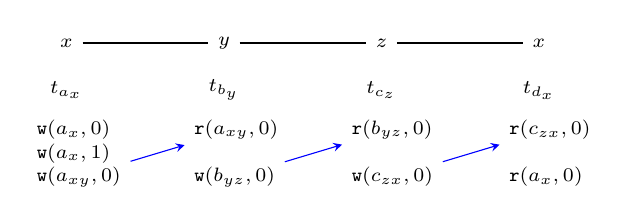
\begin{tikzpicture}
    \node (x1) at (0,0) {\scriptsize $x$};
    \node (y) at (2, 0) {\scriptsize $y$};
    \node (z) at (4, 0) {\scriptsize $z$};
    \node (x2) at (6, 0) {\scriptsize $x$};
    \draw [thin] (x1) to (y) to (z) to (x2);

    \begin{scope}[yshift=-0.6cm]
    \node (a) at (0,0) {\scriptsize $t_{a_x}$};
    \node (b) at (2, 0) {\scriptsize $t_{b_y}$};
    \node (c) at (4, 0) {\scriptsize $t_{c_z}$};
    \node (d) at (6, 0) {\scriptsize $t_{d_x}$};
    %\draw [thin] (a) to (b) to (c) to (d);

    \node [right] at (-0.5, -0.5) {\scriptsize $\wt(a_x, 0)$};
    \node [right] at (-0.5, -0.8) {\scriptsize $\wt(a_x, 1)$};
    \node [right] (1) at (-0.5, -1.1) {\scriptsize $\wt(a_{xy}, 0)$};

    \node [right] (2) at (1.5, -0.5) {\scriptsize $\rd(a_{xy}, 0)$};
    \node [right] (3) at (1.5, -1.1) {\scriptsize $\wt(b_{yz}, 0)$};

    \draw [blue, ->, >=stealth] (1) to  (2);

    \node [right] (4) at (3.5, -0.5) {\scriptsize $\rd(b_{yz}, 0)$};
    \node [right] (5) at (3.5, -1.1) {\scriptsize $\wt(c_{zx}, 0)$};
    \draw [blue, ->, >=stealth] (3) to  (4);

    \node [right] (6) at (5.5, -0.5) {\scriptsize $\rd(c_{zx}, 0)$};
    \node [right] (7) at (5.5, -1.1) {\scriptsize $\rd(a_x, 0)$};
    \draw [blue, ->, >=stealth] (5) to  (6);

    \end{scope}
  \end{tikzpicture}
  }  
  \caption{From triangles to violations of weak-read-coherence} 
  \label{fig:super-linear-illustration}
\end{figure}

Our idea for the reduction is as follows. We will construct $\expartial$ in such a way that for every $\rd(x, v)$ there is a unique $\wt(x, v)$ present in the entire program. Therefore, the $\rf$ relation is fixed. If $G$ has a triangle, we will have a shared variable $a$ and a cycle of the form: $\wt(a, 0) \xrightarrow{\po} \wt(a, 1) \xrightarrow{\hb} \rd(a, 0) \xrightarrow{\rf^{-1}} \wt(a, 0)$. This cycle violates weak-read-coherence.
If $\expartial$ with the fixed $\rf$ violates  
\WRCoh{}, then $G$ has a triangle.  The $\hb$ path $\wt(a, 1) \xrightarrow{\hb} \rd(a, 0)$ should reflect the presence of a triangle in $G$. Here is the full construction.

%The key aspect of the construction is depicted in Figure~\ref{fig:super-linear-illustration}. Suppose $G$ contains a triangle over vertices $x, y, z$. We consider a variable $a_x$ for which we extract an $\hb$ path as above. To force the $\hb$ path to have length $3$, we consider four copies $t_{a_x}, t_{b_x}, t_{c_x}, t_{d_x}$ for each vertex $x$. When there is edge $(x, y)$, thread $t_{a_x}$ writes to $t_{b_y}$. Similarly, $(y, z)$ makes $t_{b_y}$ write to $t_{c_z}$ and finally the edge $(z, x)$ makes $t_{c_z}$ write to $t_{d_x}$ which contains $\rd(a_x, 0)$. Here is the full Construction. 

\noindent{\bf{Construction}}. Given an undirected graph $G = (V_G, E_G)$ with $n$ vertices, we construct a partial execution graph $\expartial = \tup{\E, \po}$ with $|\E|=\mathcal{O}(V_G+E_G)$ such that $\expartial$ satisfies weak-read-coherence iff $G$ is triangle-free.
For simplicity, we let $V_G=\{1,\dots, n\}$. As the graph is undirected, we assume that if $(u,v) \in E$ then $(v, u) \in E$.

\smallskip 
\noindent \emph{Events, threads  and memory locations}. For each  vertex $v \in V_G$, we have threads $t_{a_v}, t_{b_v}, t_{c_v}$ and $t_{d_v}$. 
For each edge $(u,v) \in E_G$, we have locations $a_{uv}, b_{uv}, c_{uv}$. We also have locations $a_v, b_v, c_v$ for $v \in V_G$. 
The events are $\wt(a_v,0), \wt(a_v,1), \rd(a_v, 0)$, as well as $\{\wt(x_{uv},0), \rd(x_{uv},0) \mid x \in \{a,b,c\}\}$. 
We also have events $\wt(b_v),\wt(c_v)$ (the values do not matter).  
This gives us $4|V_G|$ threads, $3(|E_G|+|V_G|)$ locations and $5|V_G|+2|E_G|$ events. 

We now describe the threads. 
Let $v \in V_G$ and $x \in \{a,b, c\}$. Let $N_v=\{\alpha \mid (v, \alpha) \in E_G\}$.
Let $W(x_{vw},0), R(x_{vw},0)$ be  macros representing respectively, 
the sequence of events $\wt(x_{v\alpha_1},0) \dots \wt(x_{v\alpha_m},0)$ 
and $\rd(x_{v\alpha_1},0) \dots \rd(x_{v\alpha_m},0)$ such that 
$\alpha_1, \dots, \alpha_n \in N_v$. 

\begin{align*}
& t_{a_v}: \wt(a_v,0) \wt(a_v,1) W(a_{vw},0) \\
& t_{b_v}: R(a_{wv},0) ~w(b_v)~ W(b_{vw},0) \\
& t_{c_v}: R(b_{wv},0)~w(c_v)~W(c_{vw},0) \\
& t_{d_v}: R(c_{wv},0)\rd(a_v,0)
\end{align*}


The construction is such that each location is written into by a unique thread. Further, each location is accessed only by at most two threads. Each location (barring $a_v$) is written into exactly once by its writer thread and the $\rf$ is trivially determined. Thus, the constructed $\expartial$ qualifies as a single writer. 
The construction has the following properties. 
\begin{enumerate}
    \item $(x, y) \in E_G$ iff $\wt(a_{x},0)~\po~\wt(a_{x},1)~\hb~\wt(b_{y})$
    \item $(x, y) \in E_G$ iff $\wt(b_{x})~\hb~\wt(c_{y})$
    \item $(x, y) \in E_G$ iff $\wt(c_{x})~\hb~\rd(a_{y},0)$
\end{enumerate}


Thus, a path $x-y-z$ of length 2 results in $\wt(a_x,1)~\po~\wt(a_x,0)~\hb~\wt(b_y)~\hb~\wt(c_z)$, and  a
path $x-y-z-w$ of length 3 results in 
\[\wt(a_x,1)~\po~\wt(a_x,0)~\hb~\wt(b_y)~\hb~\wt(c_z)~\hb~\rd(a_w,0) \]

The key invariant behind the reduction is that for any $v \in V_G$, $\wt(a_v,1)~ \hb ~\rd(a_v,0)$ iff $G$ contains a triangle. The former 
violates weak-read-coherence. Figure \ref{fig:super-linear-lower-bound} shows the reduction on a graph with 3 vertices $\{1,2,3\}$, having edges between every distinct pair of vertices.  




\begin{figure*}[!htbp]
\newcommand{\xtstep}{0.3}
\newcommand{\ytstep}{0.7}
\newcommand{\ybias}{-0.3 }
\newcommand{\xstep}{1.4}
\newcommand{\ystep}{-0.6}
\newcommand{\xtscale}{0.8}
\def\crossoutopacity{0.3}
\def \numevents{5}
\def\scale{0.73}
\centering
\scalebox{\scale}{
\begin{tikzpicture}[thick,font=\footnotesize,
pre/.style={<-,shorten >= 2pt, shorten <=2pt, very thick},
post/.style={->,shorten >= 3pt, shorten <=3pt,   thick},
seqtrace/.style={line width=1},
und/.style={very thick, draw=gray},
virt/.style={circle,draw=black!50,fill=black!20, opacity=0}]
\tikzstyle{event} = [rectangle, fill=white, inner sep=0, minimum height=4.6mm, minimum width=14mm, rounded corners]

\node[] (S11) at (-5.5*\xstep,.1) {\normalsize $t_{a_1}$};
\node[] (S12) at (-5.5*\xstep,\numevents * \ystep) {};
\node[] (S21) at (-4.5*\xstep,.1) {\normalsize $t_{a_2}$};
\node[] (S22) at (-4.5*\xstep,\numevents * \ystep) {};
\node[] (S31) at (-3.5*\xstep,.1) {\normalsize $t_{a_3}$};
\node[] (S32) at (-3.5*\xstep,\numevents * \ystep) {};
\node[] (S41) at (-2.5*\xstep,.1) {\normalsize $t_{b_1}$};
\node[] (S42) at (-2.5*\xstep,\numevents * \ystep) {};
\node[] (S51) at (-1.5*\xstep,.1) {\normalsize $t_{b_2}$};
\node[] (S52) at (-1.5*\xstep,\numevents * \ystep) {};
\node[] (S61) at (-.5*\xstep,.1) {\normalsize $t_{b_3}$};
\node[] (S62) at (-.5*\xstep,\numevents * \ystep) {};
\node[] (S71) at (.5*\xstep,.1) {\normalsize $t_{c_1}$};
\node[] (S72) at (.5*\xstep,\numevents * \ystep) {};
\node[] (S81) at (1.5*\xstep,.1) {\normalsize $t_{c_2}$};
\node[] (S82) at (1.5*\xstep,\numevents * \ystep) {};
\node[] (S91) at (2.5*\xstep,.1) {\normalsize $t_{c_3}$};
\node[] (S92) at (2.5*\xstep,\numevents * \ystep) {};
\node[] (S101) at (3.5*\xstep,.1) {\normalsize $t_{d_1}$};
\node[] (S102) at (3.5*\xstep,\numevents * \ystep) {};
\node[] (S111) at (4.5*\xstep,.1) {\normalsize $t_{d_2}$};
\node[] (S112) at (4.5*\xstep,\numevents * \ystep) {};
\node[] (S121) at (5.5*\xstep,.1) {\normalsize $t_{d_3}$};
\node[] (S122) at (5.5*\xstep,\numevents * \ystep) {};



\draw[seqtrace] (S11) to (S12);
\draw[seqtrace] (S21) to (S22);
\draw[seqtrace] (S31) to (S32);
\draw[seqtrace] (S41) to (S42);
\draw[seqtrace] (S51) to (S52);
\draw[seqtrace] (S61) to (S62);
\draw[seqtrace] (S71) to (S72);
\draw[seqtrace] (S81) to (S82);
\draw[seqtrace] (S91) to (S92);
\draw[seqtrace] (S101) to (S102);
\draw[seqtrace] (S111) to (S112);
\draw[seqtrace] (S121) to (S122);




\node[event] (11) at (-5.5*\xstep, 1*\ystep + 0*\ybias) {$\wt(a_1,0)$};
\node[event] (12) at (-5.5*\xstep, 2*\ystep + 0*\ybias) {$\wt(a_1,1)$};
\node[event] (13) at (-5.5*\xstep, 3*\ystep + 0*\ybias) {$\wt(a_{12},0)$};
\node[event] (14) at (-5.5*\xstep, 4*\ystep + 0*\ybias) {$\wt(a_{13},0)$};



\node[event] (11) at (-4.5*\xstep, 1*\ystep + 0*\ybias) {$\wt(a_2,0)$};
\node[event] (12) at (-4.5*\xstep, 2*\ystep + 0*\ybias) {$\wt(a_2,1)$};
\node[event] (13) at (-4.5*\xstep, 3*\ystep + 0*\ybias) {$\wt(a_{21},0)$};
\node[event] (14) at (-4.5*\xstep, 4*\ystep + 0*\ybias) {$\wt(a_{23},0)$};



\node[event] (11) at (-3.5*\xstep, 1*\ystep + 0*\ybias) {$\wt(a_3,0)$};
\node[event] (12) at (-3.5*\xstep, 2*\ystep + 0*\ybias) {$\wt(a_3,1)$};
\node[event] (13) at (-3.5*\xstep, 3*\ystep + 0*\ybias) {$\wt(a_{31},0)$};
\node[event] (14) at (-3.5*\xstep, 4*\ystep + 0*\ybias) {$\wt(a_{32},0)$};

\node[event] (11) at (-2.5*\xstep, 1*\ystep + 0*\ybias) {$\rd(a_{31},0)$};
\node[event] (12) at (-2.5*\xstep, 2*\ystep + 0*\ybias) {$\rd(a_{21},0)$};
\node[event] (12) at (-2.5*\xstep, 3*\ystep + 0*\ybias) {$\wt(b_1)$};
\node[event] (13) at (-2.5*\xstep, 4*\ystep + 0*\ybias) {$\wt(b_{12},0)$};
\node[event] (14) at (-2.5*\xstep, 5*\ystep + 0*\ybias) {$\wt(b_{13},0)$};



\node[event] (11) at (-1.5*\xstep, 1*\ystep + 0*\ybias) {$\rd(a_{32},0)$};
\node[event] (12) at (-1.5*\xstep, 2*\ystep + 0*\ybias) {$\rd(a_{12},0)$};
\node[event] (12) at (-1.5*\xstep, 3*\ystep + 0*\ybias) {$\wt(b_2)$};
\node[event] (13) at (-1.5*\xstep, 4*\ystep + 0*\ybias) {$\wt(b_{21},0)$};
\node[event] (14) at (-1.5*\xstep, 5*\ystep + 0*\ybias) {$\wt(b_{23},0)$};

\node[event] (11) at (-.5*\xstep, 1*\ystep + 0*\ybias) {$\rd(a_{23},0)$};
\node[event] (12) at (-.5*\xstep, 2*\ystep + 0*\ybias) {$\rd(a_{13},0)$};
\node[event] (12) at (-.5*\xstep, 3*\ystep + 0*\ybias) {$\wt(b_3)$};
\node[event] (13) at (-.5*\xstep, 4*\ystep + 0*\ybias) {$\wt(b_{31},0)$};
\node[event] (14) at (-.5*\xstep, 5*\ystep + 0*\ybias) {$\wt(b_{32},0)$};


\node[event] (11) at (.5*\xstep, 1*\ystep + 0*\ybias) {$\rd(b_{31},0)$};
\node[event] (12) at (.5*\xstep, 2*\ystep + 0*\ybias) {$\rd(b_{21},0)$};
\node[event] (12) at (.5*\xstep, 3*\ystep + 0*\ybias) {$\wt(c_1)$};
\node[event] (13) at (.5*\xstep, 4*\ystep + 0*\ybias) {$\wt(c_{12},0)$};
\node[event] (14) at (.5*\xstep, 5*\ystep + 0*\ybias) {$\wt(c_{13},0)$};


\node[event] (11) at (1.5*\xstep, 1*\ystep + 0*\ybias) {$\rd(b_{32},0)$};
\node[event] (12) at (1.5*\xstep, 2*\ystep + 0*\ybias) {$\rd(b_{12},0)$};
\node[event] (12) at (1.5*\xstep, 3*\ystep + 0*\ybias) {$\wt(c_2)$};
\node[event] (13) at (1.5*\xstep, 4*\ystep + 0*\ybias) {$\wt(c_{21},0)$};
\node[event] (14) at (1.5*\xstep, 5*\ystep + 0*\ybias) {$\wt(c_{23},0)$};


\node[event] (11) at (2.5*\xstep, 1*\ystep + 0*\ybias) {$\rd(b_{23},0)$};
\node[event] (12) at (2.5*\xstep, 2*\ystep + 0*\ybias) {$\rd(b_{13},0)$};
\node[event] (12) at (2.5*\xstep, 3*\ystep + 0*\ybias) {$\wt(c_3)$};
\node[event] (13) at (2.5*\xstep, 4*\ystep + 0*\ybias) {$\wt(c_{31},0)$};
\node[event] (14) at (2.5*\xstep, 5*\ystep + 0*\ybias) {$\wt(c_{32},0)$};


\node[event] (11) at (3.5*\xstep, 1*\ystep + 0*\ybias) {$\rd(c_{31},0)$};
\node[event] (12) at (3.5*\xstep, 2.5*\ystep + 0*\ybias) {$\rd(c_{21},0)$};
\node[event] (13) at (3.5*\xstep, 4*\ystep + 0*\ybias) {$\rd(a_{1},0)$};

\node[event] (11) at (4.5*\xstep, 1*\ystep + 0*\ybias) {$\rd(c_{32},0)$};
\node[event] (12) at (4.5*\xstep, 2.5*\ystep + 0*\ybias) {$\rd(c_{12},0)$};
\node[event] (13) at (4.5*\xstep, 4*\ystep + 0*\ybias) {$\rd(a_{2},0)$};

\node[event] (11) at (5.5*\xstep, 1*\ystep + 0*\ybias) {$\rd(c_{23},0)$};
\node[event] (12) at (5.5*\xstep, 2.5*\ystep + 0*\ybias) {$\rd(c_{13},0)$};
\node[event] (13) at (5.5*\xstep, 4*\ystep + 0*\ybias) {$\rd(a_{3},0)$};

\end{tikzpicture}
}
\caption{
A partial execution $\expartial$ for a graph $G=(\{1,2,3\}, \{(1,2), (2,1),(1,3), (3,1), (2,3), (3,2)\})$. 
We have $(\wt(a_1,0), \rd(a_1,0))\in \hb$  violating weak read coherence in $\expartial$.
\label{fig:super-linear-lower-bound}
}
\end{figure*}

\noindent{\bf{Correctness and Time Complexity}}. Assume that $G$ has a triangle $(x, y, z)$. Wlg, let $x < y < z$. Then $\wt(a_x,1) ~\hb~ \rd(a_x,0)$ as follows: 
$\wt(a_x,1) ~\po ~\wt(a_{xy},0)$ $~\rf~ \rd(a_{xy},0)~\po~\wt(b_{yz},0)~\rf ~$ $\rd(b_{yz},0)~\po~\wt(c_{zx},0)~\rf~\rd(c_{zx},0)~\po~\rd(a_x,0)$ (See Figure~\ref{fig:super-linear-illustration}). 
Together with $\wt(a_x,0)~\po~\wt(a_x,1)$, we obtain a weak-read-coherence violation. 
 Triangle-freeness in the input graph $G$ ensures satisfying weak-read-coherence. In the construction, the only way to violate weak-read-coherence 
is to have $\wt(a_v,0)~\po~\wt(a_v,1)~\hb ~\rd(a_v,0)$ for some $v \in V_G$. This is achieved by:
\[ \wt(a_v,1)~\po~\wt(a_{vu},0)~\hb~\wt(b_{uw},0)~\hb~\wt(c_{wv},0)~\rf~\rd(c_{wv},0)~\po~\rd(a_v,0)\] 

This points to a triangle $v u w$ in $G$.   
The total time to construct $\expartial$ is $O(V_G+E_G)$. 
\smallskip

We have seen how the special structure of $\onewriter$ systems eliminates the combinatorial problem of synthesizing $\mo$, since the writes to each location are already totally ordered by program order. This  makes the $\vm$ problem polynomial time for $\ramm$ and its variants. On the other hand the conditional lower bound suggests that the algorithm cannot be faster than detecting triangles in a graph. The next chapter will be dedicated to hardness results for multi-writers discussed in the beginning of this chapter. 

  
\chapter{Hardness Results for VRA}
A single writer per location induced a polynomial-time algorithm for the consistency check. Here we show that having two writers per thread makes the problem $\NP$-complete. The $\NP$ upper bound follows by guessing an $\rf$ and $\mo$ and then checking whether the complete execution graph $\ex = \tuple{\E, \po, \rf, \mo}$ satisfies the consistency axioms. When $\rf$ and $\mo$ are already given, this test can be done in polynomial-time~\cite{Tunc2023}. Hence the $\NP$ upper bound follows. The hardness for our $\vm$ problem comes from the fact that we need to \emph{synthesize} suitable $\rf$ and $\mo$ (the analogue in the sequential consistency setting would be the synthesis of an interleaving). For proving hardness, we provide a reduction from 3-CNF-SAT: given a boolean formula $\varphi$ over $k$ variables and $m$ clauses, with each clause being a disjunction of three literals, is there a satisfying assignment for $\varphi$?  We provide two reductions.
\begin{enumerate}
\item Formula $\varphi$ to a partial execution graph $\expartial_\varphi$ with $\mathcal{O}(k)$ threads, and containing at most \emph{three threads} writing to a location (\threewriter). 
\item Formula $\varphi$ to a partial execution graph $\ypartial_\varphi$ with $\mathcal{O}(k + m)$ threads, and containing at most \emph{two threads} writing to a location (\twowriter). 
\end{enumerate}

In both the reductions, we achieve the property that $\varphi$ is satisfiable iff $\expartial_\varphi$ (correspondingly $\ypartial_\varphi$) are $\MemModel$-consistent, for $\MemModel \in \{\sramm, \ramm, \wramm\}$. This shows that the consistency checking problem is $\NP$-complete with a bounded number of writers per location, in fact, even with two writers. The reason we present the first reduction to \threewriter\ is because we get a stronger conditional bound: since the number of threads in $\expartial_\varphi$ is linearly related to the number of variables in $\varphi$, we get a parameterized reduction that helps proving a conditional lower bound under the Exponential Time Hypothesis (ETH). In the reduction to \twowriter\ systems, the number of threads depends both on $k$ (number of variables in the formula) and $m$ (the number of clauses). Hence this reduction cannot be used for the conditional lower bound. 
We will first describe the reduction to three writers and its implications, and then follow up with the second reduction. 

\paragraph*{Notation.} Let the variables used by $\varphi$ be $x_1, \dots, x_k$. The clauses are $C_1, \dots, C_m$. Each clause $C_j$ consists of three literals $(\ell_j^1, \ell_j^2, \ell_j^3)$, where each literal is either a variable $x_i$ or its negation $\neg x_i$. We define $S_{x_i} := \{j \mid C_j \text{ contains } x_i\}$ and $S_{\neg x_i} := \{ j \mid C_j \text{ contains } \neg x_i\}$ as the set of (indices of) clauses containing the literals $x_i$ and $\neg x_i$ respectively.

\section{Fine-grained hardness for  \threewriter\ systems}\label{sec:hardness}
\label{sec:hardness-threewriter}
We consider execution graphs where for each variable $x$ there are at most three threads writing to $x$, that is, at most three threads can have statements of the form $\wt(x, d)$. We will call them \threewriter\ execution graphs. 
Our objective is to show a hardness result stronger than $\NP$-hardness, for the $\vm$ problem under the assumption stated below.

\noindent \textbf{Exponential Time Hypothesis (ETH)}. There is no $2^{o(k)}\cdot (k+m)^{\mathcal{O}(1)}$ algorithm for 3-CNF-SAT, where $k$ is the number of variables, $m$ is the number of clauses~\cite{ImpagliazzoPZ01,Lokshtanov:ETH:2011}.

We prove the following theorem in this section. 

\begin{theorem}\label{thm:eth-hardness}
    Under ETH, there is no $2^{o(k)} \cdot n^{\mathcal{O}(1)}$ algorithm for the $\vm$-problem with $\MemModel \in \{ \sramm, \ramm, \wramm\}$, $k$ being the number of threads, and $n$ the number of events. The result holds even while restricting the input instance to \threewriter\ execution graphs.
\end{theorem}

\paragraph*{Proof strategy.} Given a 3-CNF formula $\varphi$ with $k$ threads and $m$ clauses, we construct a partial execution graph $\expartial_\varphi = \tuple{\E, \po}$ that satisfies the following properties:
\begin{itemize}
\item $\expartial_\varphi$ is \threewriter,
\item the number of threads in $\expartial_\varphi$ is $\mathcal{O}(k)$,
\item the number of events in $\expartial_\varphi$ is $\mathcal{O}(k + m)$, 
\item $\expartial_\varphi \models \MemModel$ iff $\varphi$ is satisfiable, for $\MemModel \in \{\sramm, \ramm, \wramm\}$. 
\end{itemize} 

 
\begin{figure}
\footnotesize%\noindent

\begin{tabular}{c| c}
    $T_i^1$ & $T_i^0$  \\
    $\wt(s_i, 1)$~~&~~$\wt(s_i, 1)$~~ \\
    $\wt(s_i, 2)$~~&~~$\wt(s_i, 2)$~~ \\
    $\wt(v_i, 1)$~~&~~$\wt(v_i, 0)$~~
\end{tabular}
\hfill
\begin{tabular}{c | c }
    $T_{x_i}$~ & ~$T_{\neg x_i}$ \\
        & \\
        $\rd(v_i, 1)$~&~$\rd(v_i, 0)$ \\
        & \\
        $\wt(c_j, 1)$ ~&~ $\wt(c_j, 1)$ \\
        $\forall j \in S_{x_i}$ ~&~  $\forall j \in S_{\neg x_i}$ 
\end{tabular}
\hfill
\begin{tabular}{c}
    $T_f$ \\
    $\rd(c_1, 1)$ \\
    $\cdots$ \\
    $\rd(c_m, 1)$ \\
    $\rd(s_1, 2)$ \\
    $\rd(s_1, 1)$ \\
    $\cdots$ \\
    $\rd(s_k, 2)$ \\
    $\rd(s_k, 1)$ 
\end{tabular}
 \caption{Threads in the reduction, for $i \in \{1, 2, \dots, k\}$ }
   \label{tab:reduction-threads-ra}
\end{figure}

Thus, if there was a $2^{o(k)} \cdot n^{\mathcal{O}(1)}$ algorithm for the $\vm$ problem, we could solve 3-CNF-SAT in $2^{o(k)}.(k+m)^{\mathcal{O}(1)}$ time: from $\varphi$, construct the $\vm$ instance in $\mathcal{O}(k + m)$ time, and then use the $2^{o(k)} \cdot (k+m)^{\mathcal{O}(1)}$ procedure for $\vm$, thereby contradicting ETH. To show the last item above, we make use of what is known in the literature as a \emph{range reduction}~\cite{ChakrabortyKMP24}: using Lemma~\ref{lem:sra-ra-wra-relationship}, it is enough to show that if $\varphi$ has a satisfying assignment, then $\expartial \models \sramm$, and if $\varphi$ does not have a satisfying assignment, then $\expartial \not \models \wramm$. 

\paragraph*{The reduction.} 
 For every variable $x_i$, we introduce four threads $T_i^1$, $T_i^0$, $T_{x_i}$ and $T_{\neg x_i}$, as shown in Figure~\ref{tab:reduction-threads-ra}. Apart from these, there is a special thread $T_f$. 

The statements $\wt(v_i, 1)$ and $\wt(v_i,0)$ in $T_i^1$ and $T_i^0$ encode variable $x_i$ being set to \emph{true} and \emph{false} respectively. Thread $T_{x_i}$ has a read statement $\rd(v_i,1)$ (reading \emph{true} for $x_i$) and sets all clauses containing $x_i$ to true, using the statement $\wt(c_j, 1)$ for all $j \in S_{x_i}$. Similarly, thread $T_{\neg x_i}$ reads $\rd(v_i, 0)$ (\emph{false} for $x_i$) and sets all clauses containing $\neg x_i$ to true. Finally the thread $T_{f}$ needs to make sure that all clauses are set to true, hence the read statements $\rd(c_1, 1), \dots, \rd(c_m, 1)$.  The main challenge is to encode a valid assignment, where every variable is assigned a unique truth value: to do this, we need to ensure that there are no two distinct reads $\rd(c_{j}, 1)$ and $\rd(c_\ell, 1)$ in $T_f$ which read from some $T_{x_i}$ and its negation $T_{\neg x_i}$.
This is where the rest of the statements, using $s_i$ become useful, as we elaborate in the proofs below.

\begin{lemma}\label{lem:wra-eth}
If  $\expartial_\varphi \models \wramm$, then $\varphi$ has a satisfying assignment. 
\end{lemma}
\begin{proof} 
    If $\expartial_\varphi \models \wramm$ there is an $\rf$ function which satisfies porf-acyclicity and weak-read-coherence. We need to prove that this $\rf$ encodes a valid satisfying assignment. This can be shown by proving that there are no two distinct reads $\rd(c_j, 1)$ and $\rd(c_\ell, 1)$ which read from $T_{x_i}$ and $T_{\neg x_i}$ for some variable $x_i$, since it gives the following assignment: $A(x_i) = true$ if some read event $\rd(c_j, 1)$ reads from the write in $T_{x_i}$; $A(x_i) = false$ otherwise. Moreover, the assignment $A$ is satisfying since every clause is made  true by this assignment.
    

    Let us now prove the property. Suppose $\rd(c_j, 1)$ and $\rd(c_\ell, 1)$ read from $T_{x_i}$ and $T_{\neg x_i}$ respectively. Since $\rd(c_j, 1)$ reads from $T_{x_i}$, there is an $\hb$ path from $T_i^1$ to $\rd(c_j, 1)$ due to the $\rf$ edges: $\wt(v_i, 1) \xra{\rf} \rd(v_i, 1)$ and $T_{x_i}: \wt(c_j, 1) \xra{\rf} \rd(c_j, 1)$. Similarly, there is an $\hb$ path from $T_i^0$ to $\rd(c_\ell, 1)$. Hence there is an $\hb$ path from both $T_i^1$ and $T_i^0$ to the event $\rd(s_i, 1)$ in $T_f$. Since the only matching write $\wt(s_i, 1)$ appears above $\wt(s_i, 2)$ in these threads, any assignment to $\rd(s_i, 1)$ violates weak-read-coherence, a contradiction to the hypothesis that $\rf$ satisfies weak-read-coherence.
\end{proof}

\begin{restatable}{lemma}{lemsatimpliessra}
    \label{lem:sat-implies-sra}
If $\varphi$ has a satisfying assignment, then $\expartial_\varphi \models \sramm$. 
\end{restatable}
\begin{proof}
Suppose $\varphi$ has a satisfying assignment $A$. We need to synthesize $\rf$ and $\mo$ such that the resulting execution graph satisfes porf-acyclicity, strong-write-coherence and read-coherence. Since $A$ is a satisfying assignment, for every clause $C_j$ there is a literal $\ell_j$ that is made true. Let $\rf^{-1}(\rd(c_j, 1))$ be the write event $\wt(c_j, 1)$ in $T_{\ell_j}$. Assigning writes this way introduces an $\hb$ path from $T_i^{A(x_i)}$ to $T_f$ for all variables that are indeed being utilized to make the clauses true. Importantly, there is no $\hb$ path created from $T_{i}^{\neg A(x_i)}$ to the thread $T_f$. Therefore, the read event $\rd(s_i, 2)$ can read from the write in $T_i^{A(x_i)}$ and $\rd(s_i, 1)$ can read from the unused thread $T_i^{\neg A(x_i)}$. This gives an $\rf$ which satisfies weak-read-coherence. By design of the execution graph, the $\rf$ also satisfies porf-acyclicity. For the lemma, we require to prove strong-write-coherence and read-coherence. For this we need to also synthesize an $\mo$. 
Consider any  $\mo$ relation that respects the following orders:
    \begin{itemize}[leftmargin=0.1em]
    \item $T_{i}^{A(x_i)}: \wt(s_i, 1) \xra{\mo} T_i^{\neg A(x_i)}: \wt(s_i, 1) \xra{\mo}T_{i}^{\neg A(x_i)}: \wt(s_i, 2);  T_i^{A(x_i)}: \wt(s_i, 2) \xra{\mo} T_i^{\neg A(x_i)}: \wt(s_i, 1)$,
    \item For each clause $j$ there are three threads writing $\wt(c_j, 1)$.  For each clause $C_j$ choose a specific literal $\ell_j$ that is made true by the satisfying assignment $A$. The $\mo$ relation orders the other write statements $\wt(c_j, 1)$ before $T_{\ell_j}: \wt(c_j, 1)$. 
    \end{itemize} 
A concrete example of the synthesis is presented below. It shows a complete execution graph along with the synthesis of $\rf$ and $\mo$ edges.
\paragraph*{Illustration}\label{app:hardness-example}
\begin{table}[h]
    
\noindent
\begin{minipage}{0.15\textwidth}
\centering
\begin{tabular}{c | c}
    $T_1^1$ & $T_1^0$ \\
    $\wt(s_1,1)$~& ~$\wt(s_1,1)$ \\ 
    $\wt(s_1,2)$~& ~$\wt(s_1,2)$ \\ 
    $\wt(v_1, 1)$~& ~$\wt(v_1, 0)$ \\

\end{tabular}
\vspace{.1cm}

\begin{tabular}{c | c}
    $T_2^1$ & $T_2^0$ \\
    $\wt(s_2,1)$~& ~$\wt(s_2,1)$ \\ 
    $\wt(s_2,2)$~& ~$\wt(s_2,2)$ \\ 
    $\wt(v_2, 1)$~& ~$\wt(v_2, 0)$ \\
\end{tabular}
\vspace{.1cm}

\begin{tabular}{c | c}
    $T_3^1$ & $T_3^0$ \\
    $\wt(s_3,1)$~& ~$\wt(s_3,1)$ \\ 
    $\wt(s_3,2)$~& ~$\wt(s_3,2)$ \\ 
    $\wt(v_3, 1)$~& ~$\wt(v_3, 0)$ \\
   
\end{tabular}

\end{minipage}
\hfill
\begin{minipage}{0.15\textwidth}
\centering
\centering
\begin{tabular}{c | c}
    $T_{x_1}$ & $T_{\neg x_1}$ \\
    $\rd(v_1,1)$ ~& ~$\rd(v_1,0)$ \\ 
    $\wt(c_1,1)$~ &  \\ 
    $\wt(c_2, 1)$~&  \\

\end{tabular}
\vspace{.1cm}

\begin{tabular}{c | c}
   $T_{x_2}$ & $T_{\neg x_2}$ \\
    $\rd(v_2,1)$ ~& ~$\rd(v_2,0)$ \\ 
    $\wt(c_1,1)$~ & ~$\wt(c_2,1)$ \\ 
    
\end{tabular}
\vspace{.1cm}

\begin{tabular}{c | c}
    $T_{x_3}$ & $T_{\neg x_3}$ \\
    $\rd(v_3,1)$ ~& ~$\rd(v_3,0)$ \\ 
    $\wt(c_1,1)$~ & ~$\wt(c_2,1)$ \\ 
    
   
\end{tabular}
\end{minipage}
\hfill
\begin{minipage}{0.15\textwidth}
\centering
\begin{tabular}{c}
    $T_f$ \\
    $\rd(c_1, 1)$ \\
    $\rd(c_2, 1)$ \\
    $\rd(s_1, 2)$ \\
    $\rd(s_1, 1)$ \\
    $\rd(s_2, 2)$ \\
    $\rd(s_2, 1)$ \\
    $\rd(s_3, 2)$ \\
    $\rd(s_3, 1)$ \\

\end{tabular}
\end{minipage}
\vspace{2em}
\caption{$\varphi=(x_1\lor x_2\lor x_3)\land (x_1 \lor \neg x_2\lor \neg x_3)$}
    \label{tab:example-finegrainedwra}
\end{table}

Table~\ref{tab:example-finegrainedwra} gives an instance of the construction of $\expartial$ for the fine-grained hardness reduction for \threewriter~ and (Figure~\ref{example-Execution-ra}) gives the complete execution graph for it. The execution graph is constructed for $x_1=1, x_2=0, x_3=0$, a satisfying assignment for $\varphi$. The $\rf$ and $\mo$-edges follow the rule of construction for them given in the reduction we discussed before. The $\rf$ synthesis is as follows:
\begin{itemize}
    \item $\tuple{T_{x_1}:\wt(c_1,1)}~\rf~\tuple{T_f:\rd(c_1,1)}$, $\tuple{T_{x_1}:\wt(c_2,1)}~\rf~\tuple{T_f:\rd(c_2,1)}$
    \item $\tuple{T_1^1:\wt(s_1,2)}~\rf~\tuple{T_f:\rd(s_1,2)}$, $\tuple{T_1^0:\wt(s_1,1)}~\rf~\tuple{T_f:\rd(s_1,1)}$
    \item $\tuple{T_2^0:\wt(s_2,2)}~\rf~\tuple{T_f:\rd(s_2,2)}$, $\tuple{T_2^1:\wt(s_2,1)}~\rf~\tuple{T_f:\rd(s_2,1)}$
    \item $\tuple{T_3^0:\wt(s_3,2)}~\rf~\tuple{T_f:\rd(s_3,2)}$, $\tuple{T_3^1:\wt(s_3,1)}~\rf~\tuple{T_f:\rd(s_3,1)}$
\end{itemize}

All other $\rf$-edges are trivial. They are not reflected in Figure~\ref{example-Execution-ra}. Let us construct the $\mo$-edges.
\begin{itemize}
 \item $\tuple{T_1^1:\wt{s_1,2}} \xra{\mo}\allowbreak \tuple{T_1^0:\wt{s_1,1}}$ , $\tuple{T_1^1:\wt{s_1,1}} \xra{\mo}\allowbreak \tuple{T_1^0:\wt{s_1,1}}$
 
 \item $\tuple{T_j^0:\wt{s_j,2}} \xra{\mo}\allowbreak \tuple{T_j^1:\wt{s_j,1}}$, $\tuple{T_j^0:\wt{s_j,1}} \xra{\mo}\allowbreak \tuple{T_j^1:\wt{s_j,1}}$ for $j=2,3$
 
 \item $\tuple{T_{x_j}:\wt{c_1,1}} \xra{\mo}\allowbreak \tuple{T_{x_1}:\wt{c_1,1}}$, $\tuple{T_{x_j}:\wt{c_2,1}} \xra{\mo}\allowbreak \tuple{T_{x_1}:\wt{c_2,1}}$ for $j=1,2$.
\end{itemize}

Other $\mo$ edges follow the direction of $\po$ and are not explicitly constructed in Figure~\ref{example-Execution-ra}. %Note that the resulting execution graph satisfies all the memory axioms of $\sramm$ (Refer Table~\ref{table:ax:models-2}).


\begin{figure*}% 
\begin{center}
 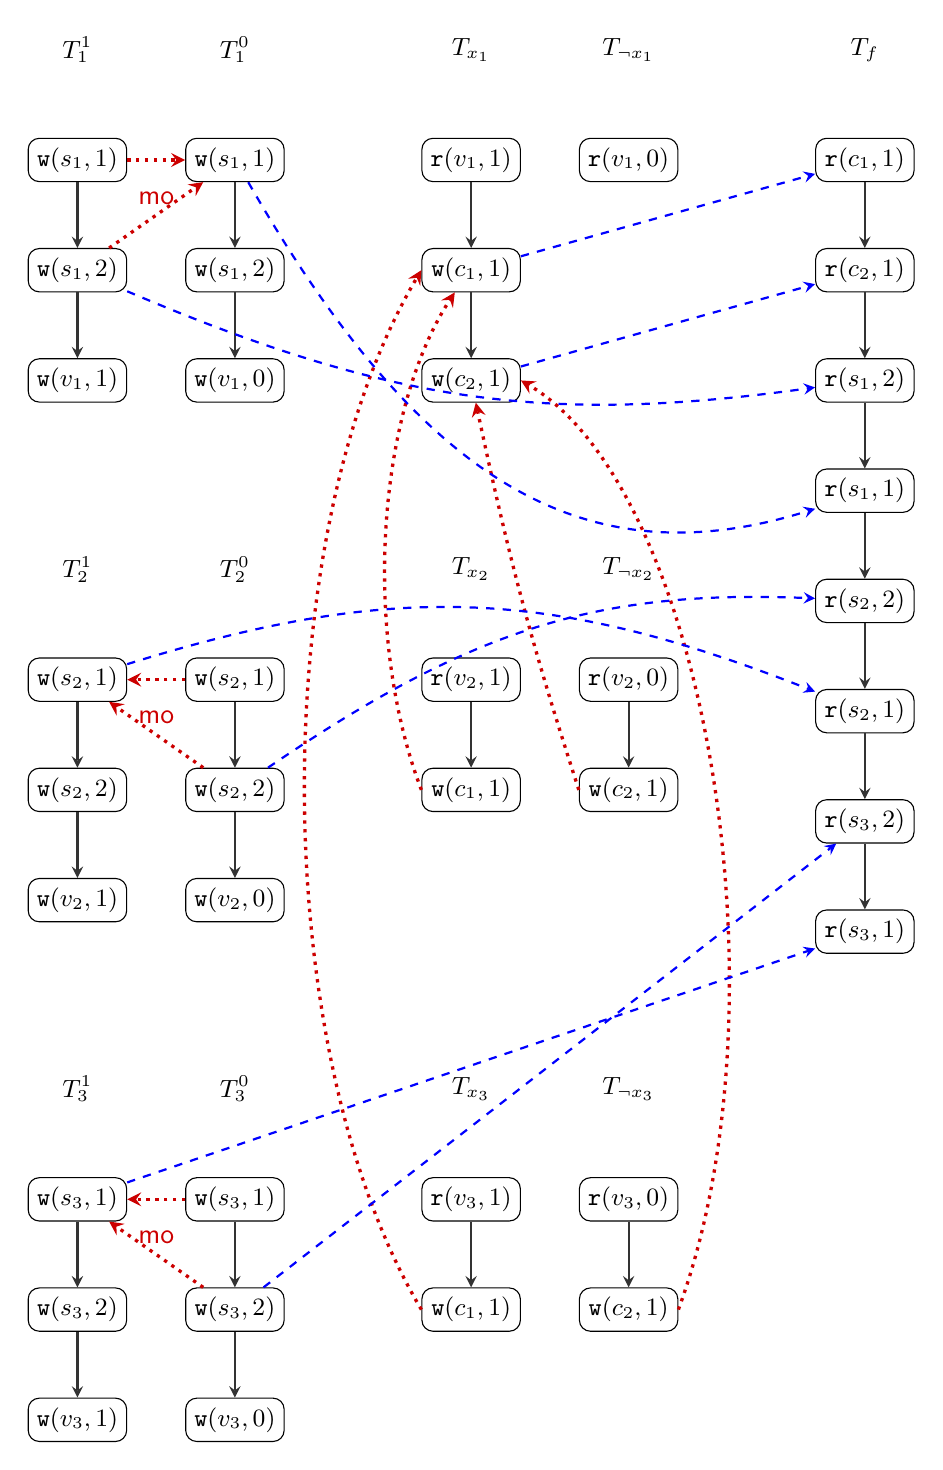
\begin{tikzpicture}[scale =1,yscale=2, 
    op/.style={draw, fill=white, rounded corners, minimum width=1.25cm, minimum height=0.55cm, 
               inner sep=2pt, font=\small},
    thread/.style={font=\small\bfseries},
    >=stealth
]

% ------------------------------------------------------------
% First group: T_i^1 and T_i^0
% ------------------------------------------------------------

% T_1^1 / T_1^0
\node[thread] (T11) at (0, 0.9) {$T_1^1$};
\node[thread] (T10) at (2.0, 0.9) {$T_1^0$};

\node[op] (s11a) at (0, 0.2) {$\wt(s_1,1)$};
\node[op] (s11b) at (0,-0.5) {$\wt(s_1,2)$};
\node[op] (v11)  at (0,-1.2) {$\wt(v_1,1)$};

\draw[po] (s11a) to (s11b);
\draw[po] (s11b) to (v11);



\node[op] (s10a) at (2.0, 0.2) {$\wt(s_1,1)$};
\node[op] (s10b) at (2.0,-0.5) {$\wt(s_1,2)$};
\node[op] (v10)  at (2.0,-1.2) {$\wt(v_1,0)$};

\draw[po] (s10a) to (s10b);
\draw[po] (s10b) to (v10);

\draw[mo] (s11b) to node[above] {$\mo$} (s10a);
\draw[mo] (s11a) to (s10a);

% T_2^1 / T_2^0
\node[thread] (T21) at (0,-2.4) {$T_2^1$};
\node[thread] (T20) at (2.0,-2.4) {$T_2^0$};

\node[op] (s21a) at (0,-3.1) {$\wt(s_2,1)$};
\node[op] (s21b) at (0,-3.8) {$\wt(s_2,2)$};
\node[op] (v21)  at (0,-4.5) {$\wt(v_2,1)$};

\draw[po] (s21a) to (s21b);
\draw[po] (s21b) to (v21);

\node[op] (s20a) at (2.0,-3.1) {$\wt(s_2,1)$};
\node[op] (s20b) at (2.0,-3.8) {$\wt(s_2,2)$};
\node[op] (v20)  at (2.0,-4.5) {$\wt(v_2,0)$};

\draw[po] (s20a) to (s20b);
\draw[po] (s20b) to (v20);
\draw[mo] (s20b) to node[above] {$\mo$} (s21a);
\draw[mo] (s20a) to (s21a);

% T_3^1 / T_3^0
\node[thread] (T31) at (0,-5.7) {$T_3^1$};
\node[thread] (T30) at (2.0,-5.7) {$T_3^0$};

\node[op] (s31a) at (0,-6.4) {$\wt(s_3,1)$};
\node[op] (s31b) at (0,-7.1) {$\wt(s_3,2)$};
\node[op] (v31)  at (0,-7.8) {$\wt(v_3,1)$};

\draw[po] (s31a) to (s31b);
\draw[po] (s31b) to (v31);

\node[op] (s30a) at (2.0,-6.4) {$\wt(s_3,1)$};
\node[op] (s30b) at (2.0,-7.1) {$\wt(s_3,2)$};
\node[op] (v30)  at (2.0,-7.8) {$\wt(v_3,0)$};

\draw[po] (s30a) to (s30b);
\draw[po] (s30b) to (v30);
\draw[mo] (s30b) to node[above] {$\mo$} (s31a);
\draw[mo] (s30a) to (s31a);
% ------------------------------------------------------------
% Second group: T_xi and T_not xi
% ------------------------------------------------------------

% T_x1 / T_not x1
\node[thread] (Tx1)  at (5.0, 0.9) {$T_{x_1}$};
\node[thread] (Tnx1) at (7.0, 0.9) {$T_{\neg x_1}$};

\node[op] (rv11) at (5.0,0.2) {$\rd(v_1,1)$};
\node[op] (c11)  at (5.0,-0.5) {$\wt(c_1,1)$};
\node[op] (c21)  at (5.0,-1.2) {$\wt(c_2,1)$};

\draw[po] (rv11) to (c11);
\draw[po] (c11) to (c21);

\node[op] (rv10) at (7.0,0.2) {$\rd(v_1,0)$};

% T_x2 / T_not x2
\node[thread] (Tx2)  at (5.0,-2.4) {$T_{x_2}$};
\node[thread] (Tnx2) at (7.0,-2.4) {$T_{\neg x_2}$};

\node[op] (rv21) at (5.0,-3.1) {$\rd(v_2,1)$};
\node[op] (c12)  at (5.0,-3.8) {$\wt(c_1,1)$};

\draw[po] (rv21) to (c12);


\node[op] (rv20) at (7.0,-3.1) {$\rd(v_2,0)$};
\node[op] (c22)  at (7.0,-3.8) {$\wt(c_2,1)$};

\draw[po] (rv20) to (c22);

% T_x3 / T_not x3
\node[thread] (Tx3)  at (5.0,-5.7) {$T_{x_3}$};
\node[thread] (Tnx3) at (7.0,-5.7) {$T_{\neg x_3}$};

\node[op] (rv31) at (5.0,-6.4) {$\rd(v_3,1)$};
\node[op] (c13)  at (5.0,-7.1) {$\wt(c_1,1)$};

\draw[po] (rv31) to (c13);

\node[op] (rv30) at (7.0,-6.4) {$\rd(v_3,0)$};
\node[op] (c23)  at (7.0,-7.1) {$\wt(c_2,1)$};

\draw[po] (rv30) to (c23);
\draw[mo, bend left=45] (c12.west) to (c11);
\draw[mo, bend left=5] (c22.west) to (c21);
\draw[mo, bend left=50] (c13.west) to (c11.west);
\draw[mo, bend right=55] (c23.east) to (c21.east);

% ------------------------------------------------------------
% Final thread T_f
% ------------------------------------------------------------

\node[thread] (Tf) at (10.0,0.9) {$T_f$};

\node[op] (fc1) at (10.0,0.2) {$\rd(c_1,1)$};
\node[op] (fc2) at (10.0,-0.5) {$\rd(c_2,1)$};
\node[op] (fs12) at (10.0,-1.2) {$\rd(s_1,2)$};
\node[op] (fs11) at (10.0,-1.9) {$\rd(s_1,1)$};
\node[op] (fs22) at (10.0,-2.6) {$\rd(s_2,2)$};
\node[op] (fs21) at (10.0,-3.3) {$\rd(s_2,1)$};
\node[op] (fs32) at (10.0,-4.0) {$\rd(s_3,2)$};
\node[op] (fs31) at (10.0,-4.7) {$\rd(s_3,1)$};

%po for Tf
\draw[po] (fc1) to (fc2);
\draw[po] (fc2) to (fs12);
\draw[po] (fs12) to (fs11);
\draw[po] (fs11) to (fs22);
\draw[po] (fs22) to (fs21);
\draw[po] (fs21) to (fs32);
\draw[po] (fs32) to (fs31);

%rf edges

\draw[rf] (c11) to (fc1);
\draw[rf] (c21) to (fc2);
\draw[rf, bend right=8] (s11b) to (fs12);
\draw[rf, bend right=25] (s10a) to (fs11);
\draw[rf, bend left=10] (s20b) to (fs22);
\draw[rf, bend left=10] (s21a) to (fs21);
\draw[rf, bend left=0] (s30b) to (fs32);
\draw[rf, bend left=0] (s31a) to (fs31);
\end{tikzpicture}%
\end{center}
\caption{Execution graph for Table~\ref{tab:example-finegrainedwra}:The trivial $\rf$-edges are omitted}
\label{example-Execution-ra}
\end{figure*}%
 


It can be shown that the constructed $\rf$ and $\mo$ satisfy strong-write-coherence and read-coherence.

\paragraph*{Strong-write-coherence.} We will show that the constructed $\rf$ and $\mo$ satisfy strong-write-coherence, that is acyclicity of $\hb \cup
 \mo$. Suppose not. There is a cycle $\mathcal{C}$ consisting of $\po$, $\rf$ and $\mo$ edges (thereby violating strong-write-coherence). Since we have seen that there is no $\po \cup \rf$ cycle, cycle $\mathcal{C}$ should contain an $\mo$ edge.  An edge  $\tuple{T_{i}^{A(x_i)}: \wt(s_i, 1)} ~\mo~\tuple{T_i^{\neg{A(x_i)}}: \wt(s_i, 1)}$ cannot be present in $\mathcal{C}$ since there can be no incoming $\po$ or $\rf$ edge to $\tuple{T_{i}^{A(x_i)}: \wt(s_i, 1)}$. Now, consider an edge $\tuple{T_{i}^{A(x_i)}: \wt(s_i, 2)}~\mo~\allowbreak \tuple{T_{i}^{\neg{A(x_i)}}: \wt(s_i, 1)}$. 
  The only incoming edge to $\tuple{T_{i}^{A(x_i)}: \wt(s_i, 2)}$ is a $\po$ edge from $\tuple{T_{i}^{A(x_i)}: \wt(s_i, 1)}$, and there can be no $\po$ or $\rf$ edges into the latter event. Hence, even the second type of $\mo$ edges cannot be present in $\mathcal{C}$. 
This leaves us with $\mo$ edges of the form $\tuple{T_{\ell'}: \wt(c_j, 1)} ~\mo~\allowbreak  \tuple{T_{\ell_j}: \wt(c_j,1)}$. Notice that from the latter event, $\tuple{T_{\ell_j}: \wt(c_j, 1)}$ the only outgoing edges are to $T_f$, and from $T_f$, there are no outgoing edges, hence there is no path from an event in $T_f$ to $\tuple{T_{\ell'}: \wt(c_j, 1)}$. This proves that such an $\mo$ edge cannot be part of an $\hb \cup \po$ cycle too. We conclude that there are no $\hb \cup \mo$ cycles. 


    \paragraph*{Read-coherence.} Finally, we need to prove read-coherence, i.e., $\irr(\rf^{-1}; \mo_x; \hb)$. If read coherence is violated, there is a read event $r$, and two write events $w, w'$ such that $w~\rf~r$, $w~\mo~w'$ and $w'~\hb~r$. Such a violation can potentially happen on variables which have multiple write events: in our case $s_i$ and $c_j$.
    
    To do this, let us check what each reads on $s_i$ and $c_j$ observes. Note that no read observes a value that is $\mo$-overwritten in its happens-before past. 
    \begin{itemize}[leftmargin=0.1em]
    \item By construction $\tuple{T_f: \rd(s_i, 2)}$ can observe $\tuple{T_i^{A(x_i)}:\wt(s_i,2)}$ but not $\tuple{T_i^{\neg A(x_i)}:\wt(s_i,1)}$. Therefore there is no write event $\mo$-later than $\tuple{T_i^{A(x_i)}: \wt(s_i, 2)}$ that is observed by $\tuple{T_f: \rd(s_i, 2)}$. 
    \item For the read event $\tuple{T_f: \rd(s_i, 1)}$, all writes to $s_i$ except $\tuple{T_i^{\neg{A(x_i)}}: \wt(s_i, 2)}$ are visible to it. Moreover, the event $\tuple{T_i^{\neg A(x_i)}: \wt(s_i, 1)}$ that writes to it is the $\mo$-latest in the view.
    \item For the variable $c_j$, $\tuple{T_f: \rd(c_j, 1)}$ observes only the write $\tuple{T_{\ell_j}: \wt(c_j, 1)}$ when some literal literal $\ell_j$ satisfies $C_j$ under $A$. All other writes to $c_j$ occur $\mo$ before this write.
    \end{itemize}
    
    This shows that the constructed $\rf$ and $\mo$ are consistent with $\sramm$.
\end{proof}

We can modify the  construction of $\expartial_{\varphi}$ for $\threewriter$ to build an execuion graph for $\varphi$ which would have only two threads writing to each variable. This will be the task  behind the reduction to $\twowriter$ systems as we will see in the next section. 

 %%%%%%%%%NP-hardness%%%%%%%%%%
\subsection{Hardness for  \twowriter\ systems}
\label{sec:hardness-twowriter}

The reduction in Section~\ref{sec:hardness-threewriter} involved \threewriter\ systems.
Mainly, each clause variable $c_j$ was written by three threads corresponding to its three literals. Here, our objective is to prove hardness even when there are atmost two threads writing to each variable. We will now reduce 3-CNF-SAT to the consistency testing problem for \twowriter~ systems. However, in this reduction, a formula $\varphi$ with $k$ threads and $m$ clauses yields an execution graph with $\mathcal{O}(k + m)$ theads. While this still proves $\NP$-hardness, it does not give the stronger hardness under ETH, parameterized by the number of threads. 

\begin{theorem}
\label{thm:two-writer-hardness}
    The $\vm$ problem is $\NP$-complete for $\MemModel \in \{\sramm, \ramm, \wramm\}$, even when restricted to \twowriter\ execution graphs.
\end{theorem}



The key challenge in proving the hardness is to reduce the number of threads writing to each clause variable $c_j$ from three (one for each literal in the clause) to at most two, while still encoding the satisfiability of the 3-CNF formula. This can be achieved by introducing one auxiliary variable $d_j$ per clause. Suppose $C_j = (\ell_j^1 \vee \ell_j^2 \vee \ell_j^3)$. In all the reductions of Section~\ref{sec:hardness-threewriter}, there are three threads $T_{\ell_j^1}, T_{\ell_j^2}$ and $T_{\ell_j^3}$. We make the following changes to constructions of $\expartial_\varphi$ in Section~\ref{sec:hardness-threewriter}.

\begin{itemize}[leftmargin=0.1em]
\item Replace $\wt(c_j, 1)$ in $T_{\ell_j^3}$ with $\wt(d_j, 1)$, i.e., in the third literal, the write is on $d_j$.
\item Add a new thread $T_{j}$ with two events as follows: $\rd(c_j, 1)~;~\wt(d_j, 1)$
\item Finally, in $T_f$, replace all $\rd(c_j, 1)$ with $\rd(d_j, 1)$
\end{itemize}
Figure~\ref{fig:two-writer} reflects the changes and the full thread construction for the reduction to $\twowriter$.

\begin{figure}[t]
\centering
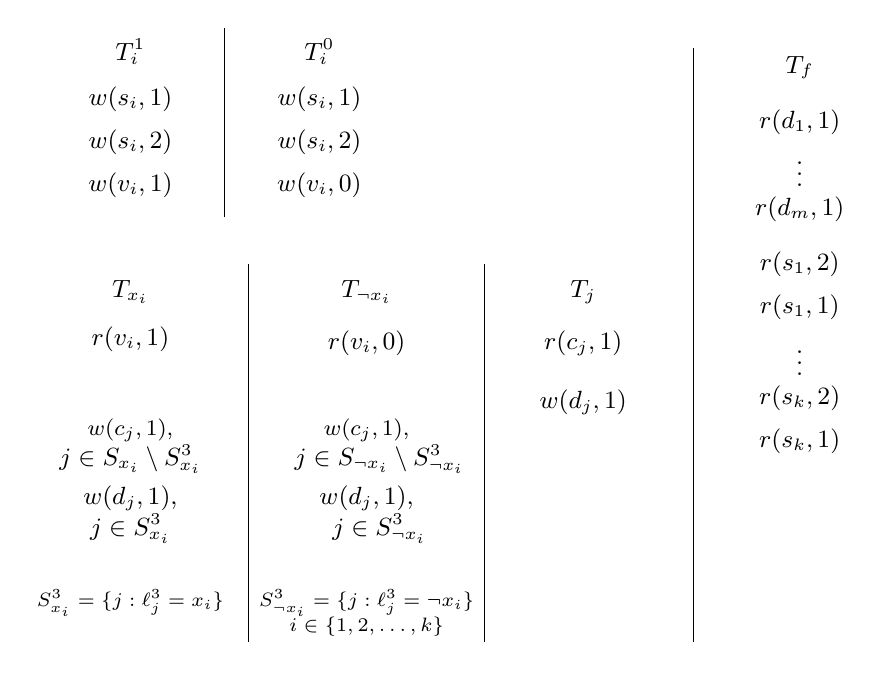
\begin{tikzpicture}[
    every node/.style={font=\small}
]

% =========================================================
% T_i^{1}
% =========================================================

\node at (0,0) {$T_i^1$};

\node at (0,-0.60) {$w(s_i,1)$};
\node at (0,-1.15) {$w(s_i,2)$};
\node at (0,-1.70) {$w(v_i,1)$};


% =========================================================
% T_i^{0}
% =========================================================

\node at (2.4,0) {$T_i^0$};

\node at (2.4,-0.60) {$w(s_i,1)$};
\node at (2.4,-1.15) {$w(s_i,2)$};
\node at (2.4,-1.70) {$w(v_i,0)$};


% vertical separator
\draw (1.2,0.30) -- (1.2,-2.10);


% =========================================================
% T_{x_i}
% =========================================================

\node at (0,-3.05) {$T_{x_i}$};

\node at (0,-3.65) {$r(v_i,1)$};

\node[align=center] at (0,-5.45)
{
\footnotesize $w(c_j,1)$,\\ $j\in S_{x_i}\setminus S_{x_i}^{3}$\\[3pt]
$w(d_j,1)$,\\
$j\in S_{x_i}^{3}$
};



\node[align=center] at (0,-7)
{\scriptsize $S_{x_i}^{3}=\{j:\ell_j^3=x_i\}$};


% =========================================================
% T_{\neg x_i}
% =========================================================

\node at (3.0,-3.05) {$T_{\neg x_i}$};

\node at (3.0,-3.70) {$r(v_i,0)$};

\node[align=center] at (3.0,-5.45)
{
\footnotesize $w(c_j,1)$,\\ \quad $j\in S_{\neg x_i}\setminus S_{\neg x_i}^{3}$\\[3pt]
$w(d_j,1)$,\\ \quad $j\in S_{\neg x_i}^{3}$
};

\node[align=center] at (3.0,-7)
{\scriptsize $S_{\neg x_i}^{3}=\{j:\ell_j^3=\neg x_i\}$};



% vertical separator
\draw (1.50,-2.70) -- (1.50,-7.5);


% =========================================================
% T_j
% =========================================================

\node at (5.75,-3.05) {$T_j$};

\node at (5.75,-3.70) {$r(c_j,1)$};
\node at (5.75,-4.45) {$w(d_j,1)$};


% vertical separator
\draw (4.50,-2.70) -- (4.50,-7.5);


% =========================================================
% T_f
% =========================================================

\node at (8.5,-0.20) {$T_f$};

\node at (8.5,-0.90) {$r(d_1,1)$};
\node at (8.5,-1.45) {$\vdots$};
\node at (8.5,-2.00) {$r(d_m,1)$};

\node at (8.5,-2.70) {$r(s_1,2)$};
\node at (8.5,-3.25) {$r(s_1,1)$};

\node at (8.5,-3.85) {$\vdots$};

\node at (8.5,-4.40) {$r(s_k,2)$};
\node at (8.5,-4.95) {$r(s_k,1)$};


% vertical separator
\draw (7.15,0.05) -- (7.15,-7.5);


% =========================================================
% Index
% =========================================================

\node at (3,-7.3)
{\scriptsize $i\in\{1,2,\ldots,k\}$};


\end{tikzpicture}

\caption{Threads in the 2-Writer reduction, for
$i\in\{1,2,\ldots,k\}$.}
\label{fig:two-writer}
\end{figure}


Notice that due to the introduction of the new threads $T_j$, the total number of threads also depends on the number of clauses $m$. Let the resulting partial execution graph be called $\ypartial_\varphi$. Then we want to show that $\varphi$ has a satisfying assignment iff $\ypartial_\varphi$ has a complete execution that satisfies the axioms of $\sramm$, $\ramm$ and $\wramm$. We again use range reduction to prove the following two lemmas.

\begin{lemma}
If  $\ypartial_\varphi \models \wramm$, then $\varphi$ has a satisfying assignment. 
\end{lemma}
\begin{proof}
The proof proceeds similar to Lemma~\ref{lem:wra-eth}. We need to argue that if there is an $\rf$ that satisfies weak-read-coherence, then there cannot be two distinct reads $\rd(d_{j}, 1)$ and $\rd(d_{p}, 1)$ in $T_f$ that (directly or indirectly) read from threads corresponding to both a literal and its negation for some variable $x_i$. The $\rd(d_j, 1)$ event in $T_f$ can either read from  $T_{\ell_j^3}$ or from $T_{j}$. Similarly, $\rd(d_p, 1)$ can read from $T_{\ell_p^3}$ or $T_p$. If it so happens that the two threads from which $\rd(d_{j}, 1)$ and $\rd(d_{p}, 1)$ read from are of the form $T_{x_i}$ and $T_{\neg x_i}$, then both $\tuple{T_i^0: \wt(s_i, 2)}$ and $\tuple{T_i^1: \wt(s_i, 2)}$ are in the view of $\tuple{T_f: \rd(s_i, 2)}$. Then, since the execution satisfies weak-read-coherence, there is no write event available for $\tuple{T_f: \rd(s_i, 1)}$. A contradiction. Hence the set of literals making the clauses true in $T_f$ encode a satisfying assignment. 
\end{proof}

\begin{lemma}
If $\varphi$ has a satisfying assignment, then $\ypartial_\varphi^{\ramm} \models \sramm$. 
\end{lemma}
\begin{proof}
Let $A$ be a satisfying assignment. The $\rf$ and $\mo$ relations on events with variables $s_i$ remains the same as in the proof of Lemma~\ref{lem:sat-implies-sra}. There are changes for $c_j$ and $d_j$. Consider a clause $C_j$.
\begin{itemize}
\item If $A$ makes $\ell_j^3$ true then:
\begin{itemize}
\item $\tuple{T_{\ell_j^3}: \wt(d_j, 1)}~\rf~\tuple{T_f: \rd(d_j, 1)}$,
\item Choose an arbitrary $\wt(c_j, 1)$ for $\tuple{T_j: \rd(c_j, 1)}$
\end{itemize}
\item Else, $A$ makes one of the first two literals of $C_j$ true. Arbitrarily pick one $\ell_j^i$, for $i \in \{1,2\}$:  
\begin{itemize}
\item $\tuple{T_{\ell_j^i}: \wt(c_j, 1)}~\rf~ \tuple{T_j: \rd(c_j, 1)}$,
\item $\tuple{T_{j}:\wt(d_j, 1)}~\rf~\tuple{T_f: \rd(d_j, 1)}$
\end{itemize}
\end{itemize}
For every variable-value pair, there are atmost two writes. With the $\rf$ picked as above, the $\mo$ relation gets fixed: the unused write is $\mo$-before the used write.

Clearly, the $\rf$ relation agrees with $\po$ and hence does not violate porf-acyclicity. We need to prove strong-write-coherence and read-coherence as in the proof of Lemma~\ref{lem:sat-implies-sra}.

\paragraph*{Strong-write-coherence.} 
Suppose, for contradiction, that there is a cycle in $\hb \cup \mo$. As in Lemma~\ref{lem:sat-implies-sra}, the only possible $\mo$ edges are between the two writes to $s_i$, $c_j$, or $d_j$. For $s_i$, the argument is identical to the $\threewriter$ case: the only incoming edges to the earlier write are from $\po$, and there are no cycles. For $c_j$ and $d_j$, each has at most two writers, and the $\mo$-later event leads to $T_f$ from which there is no path back to the $\mo$-earlier event. Thus, no cycle can be formed. Therefore, strong-write-coherence holds.

\paragraph*{Read-coherence.}
Suppose, for contradiction, that there is a violation of read-coherence: there exists a read $r$ and two writes $w, w'$ to the same variable such that $w~\rf~r$, $w~\mo~w'$, and $w'~\hb~r$. As before, this can only occur for variables $s_i$, $c_j$, or $d_j$. For $s_i$, the argument is unchanged from Lemma~\ref{lem:sat-implies-sra}. For $c_j$ and $d_j$, the view of each read contains only the $\rf$-used write, and the other write (if any) is $\mo$-before and not visible to the read. Thus, no such violation can occur.

The above two lemmas show that the constructed $\rf$ and $\mo$ are consistent with $\sramm$. 
\end{proof}

\smallskip
\section{Discussion}\label{ra-discuss}

We have presented a trichotomy of the landscape, with $\onewriter$ solved in polynomial-time, $\twowriter$ being NP-complete, and $\threewriter$ having a stronger lower bound under the Exponential-Time-Hypothesis (ETH). Our presentation works for $\ramm$ and its close variants $\sramm$ and $\wramm$.

A milder variant of the problem studies the complexity when the reads-from relation $\rf$ is also given. Then the question is to synthesize an mo such that the axioms can be satisfied. This “$\rf$-given” problem can be solved in polynomial time \cite{Tunc2023}, under no restrictions on the execution graphs. When rf is not provided
apriori, while the general problem is known to be NP-hard \cite{gibbons}, no subclass or
bounded variant with a polynomial-time algorithm is known in the literature (to
the best of my knowledge). We have shown that the $\onewriter$ subclass lends itself to a polynomial-time algorithm. In the next chapter we shall look at the $\rlxmm$ version of the $\vm$ problem and obtain similar trichotomy of results. 
 
%\input{app-hardness.tex}
%%%%%%%%%%%%% 
\chapter{Verifying Relaxed Memory Model}
\label{app:relaxed}

The relaxed memory model is a fragment of RC20 memory model,  introduced by Margalit and Lahav 2021 \cite{Margalit:2021} which defines a rich fragment of the C11 model consisting of acquire/release and relaxed accesses.  Consistency testing for $\rlxmm$ is known to be polynomial time when number of threads, variables and values are fixed. But for the stronger version of $\rlxmm$ where \PORF{} is allowed, the problem becomes NP-Complete \cite{ChakrabortyKMP24}. Please refer to Table~\ref{table:ax:models-2-app} for the axioms for $\rlxmm$-Acyclic. 
In this chapter, we study the complexity of the $\vm$- problem for both the `Relaxed' and the 'Relaxed-Acyclic' fragment of C-11. Relaxed model satisfy the coherence axioms: \RlxRCoh{} and \RlxWCoh{}  (Table~\ref{table:ax:models-2-app}). Essentially all $\hb$'s in \WRCoh{} and \WCoh{} are replaced by $\po$.  Figure~\ref{fig:relaxed-illust-app} recalls the instances for violation of the relaxed axioms.     The overview of this chapter is as follows:
\begin{itemize}
 \item Section~\ref{sec-onewriter-relaxed} gives a  $\mathcal{O}(n^3)$ algortihm for the $\vm$-problem restricted to  \onewriter~ under $\rlxmm$-Acyclic memory model.
 
 \item Section~\ref{sec:finegrained-relaxed} gives a conditional lower bound of $2^{o(k)}\dot n^{O(1)}$ under ETH for the $\vm$-problem restricted to  \threewriter.
 
 \item Section~\ref{sec:np-relaxed} shows that the $\vm$-problem restricted to \twowriter~ is NP-Complete.
\end{itemize}

\begin{table}
    \caption{\small Coherence Axioms for $\rlxmm$-Acyclic variant of C11}
    \label{table:ax:models-2-app}
    \centering
    %\small
    \begin{tabular}{lr}
   % \multicolumn{2}{c}{\underline{Release-Acquire}} \\
    %$\irr(\mo_x;\hb)$ & (\WCoh{})\\
    %$\acy(\hb \cup \mo)$ & (\SWCoh{})\\
    %$\irr(\rf^{-1};\mo_x;\hb)$ & (\RCoh{})\\
    %$\irr(\hb_x;[\W];\hb_x;\rf^{-1})$ & (\WRCoh{})\\
    %\hline
    \multicolumn{2}{c}{\underline{Relaxed-Acyclic}} \\
    $\irr(\po\cup\rf)$ & (\PORF{})\\
    $\irr(\mo_x;\po)$ & (\RlxWCoh{})\\
    $\irr(\rf^{-1};\mo_x;\rf^?;\po)$ & (\RlxRCoh{})\\
    \end{tabular}
\end{table}
The next section contains the PTIME-algorithm for $\onewriter$ systems along with its proof of correctness and complexity. The hardness results with relevant theorems will be presented in the following sections. 
\iffalse
\begin{table}
     \caption{\small The C11 models $\wramm, \ramm, \sramm, \rlxmm$.}
    \label{table:ax:models-2-app}
     
        \setlength\tabcolsep{7.5pt}
      \begin{tabular}{lr|lr}
      \multicolumn{2}{l|}{} & \multicolumn{2}{l}{} \\
      $\wramm$ & \makecell{\PORF{}\\ \WRCoh{}} &$\rlxmm$ & \makecell{\PORF{}\\ \RlxRCoh\\ \RlxWCoh} \\ 
      \hline
      $\ramm$ & \makecell{\PORF{} \\
      \WCoh{}\\ \RCoh{}}   &$\sramm$ & \makecell{\PORF{}\\ \SWCoh{}\\ \RCoh{}}\\ 
      \cline{1-4}
      %$\sramm$ & \makecell{\SWCoh{}\\ \RCoh{}} & & \\ 
      \end{tabular}
          
  \end{table}
\fi
 \begin{figure}[t]
    \def\ystep{0.4}
    \centering
     \resizebox{0.5\textwidth}{!}{
	\begin{tikzpicture}[yscale=1]
	
      \node (t11) at (12.3,0*\ystep)  {$\wt_1(x)$};
      \node (t12) at (12.3,-4*\ystep) {$\wt_2(x)$};
      \node (t0) at (12.3,-5*\ystep) {$(a)$};
      \draw[mo] (t12) to[bend left=45] node[left]{$\mo$} (t11);
    %  \draw[po] (t12) to (t13);
    %  
      \draw[po] (t11) to (t12);
    %%%%%%%%%%%%%%%%%%%%%%%%%%%%%%%%%%%%%%%%%%%%%%%%%%%%%%%%%%%%%%%%%%%%%%%%%%%%%%%%%
     \node (t11) at (16.3,0*\ystep)  {$\wt_1(x)$};
      \node (t12) at (16.3,-4*\ystep) {$\wt_2(x)$};
    %  \node (t13) at (0,-4.5*\ystep) {$\rd(x)$};
    %
      \node (t21) at (18.1,0*\ystep) {$\rd_2(x)$};
      \node (t22) at (18.1,-4*\ystep) {$\rd_1(x)$};
      \node (t1) at (17.2,-5*\ystep) {$(b)$};
    %
      \draw[mo] (t11) to node[left]{$\mo$} (t12);
    %  \draw[po] (t12) to (t13);
    %  
      \draw[po] (t21) to (t22);
    %  \draw[po] (t22) to (t23);
    %
    %  \draw[rf,bend left=0] (t11) to node[below,pos=0.9, sloped]{$\rf$} (t23);
    %  \draw[rf,bend right=0] (t21) to node[below,pos=0.9, sloped]{$\rf$} (t13);
    %    
      \draw[rf,bend left=0] (t12) to node[above, pos=.8, sloped]{$\rf$}(t21);
      \draw[rf,bend right=0] (t11) to node[below,pos=0.8, sloped]{$\rf$} (t22);
    
    \end{tikzpicture}
	 }
    \caption{Violation of (a)~\RlxWCoh:$\wt_2(x)~\mo~\wt_1(x), \wt_1(x)~\po~\wt_2(x)$ (b)~\RlxRCoh{}: $\wt_1(x)~\mo~\wt_2(x)$, $\rd_2(x)~\po~\rd_1(x)$ 
      with $\wt_2(x)~\rf~\rd_2(x)$ and $\wt_1(x)~\rf~\rd_1(x)$.}
      \label{fig:relaxed-illust-app}
\end{figure}



\section{Polynomial Time for \onewriter\ systems}\label{sec-onewriter-relaxed}
Here we give a polynomial time algorithm for solving  the $\vm$-problem for \onewriter~ under $\rlxmm$-Acyclic memory model. Note that as $\rlxmm$-Acyclic is stronger than $\rlxmm$, any polynomial time result for $\rlxmm$-Acyclic would also hold for $\rlxmm$.
As for \onewriter~ systems we have $\mo=\po$, \RlxWCoh{} would always hold. Hence to show that an execution graph $\expartial$ is $\rlxmm$-Acyclic-consistent, we need to verify \PORF{} and \RlxRCoh{}. We can state the following lemma for $\rlxmm$-Acyclic similar to  Lemma~\ref{lem:onewriter-axioms-two-properties} of Chapter~\ref{RA-ptime}. For $\rlxmm$, as \PORF{} is not required, only the second part of the lemma is meaningful and proof is same.

\begin{restatable}{lemma}{lemmaonewriterrelaxedtwoproperties-relaxed}
    \label{lem:relaxed-onewriter-axioms-two-properties}
Let $\rf_1$ and $\rf_2$ be two reads-from functions over a partial \onewriter\ execution graph $\ex=(\E, \po, \mo)$ s.t. $\mo$ agrees with $\po$. 
\begin{itemize}
\item Suppose $\rf_1 \sqsubseteq \rf_2$. Then, if $\rf_1$ induces a $\po \cup \rf_1$ cycle, then $\rf_2$ induces a $\po \cup \rf_2$ cycle.
\item Suppose both $\rf_1$ and $\rf_2$ satisfy relaxed-read-coherence. Then, the $\rf$ function $\min(\rf_1, \rf_2)$ also satisfies relaxed-read-coherence.
\end{itemize} 
\end{restatable}
\begin{proof}
 The proof for the first part is same as that of $\wramm$ in lemma~\ref{lem:onewriter-axioms-two-properties} and hence we skip it.
 
 For the second part, we denote $\rf_0=min(\rf_1,\rf_2)$. We shall show that that if $\rf_0$ violates relaxed-read-coherence, then either $\rf_1$ or $\rf_2$ violates it. Suppose $\rf_0$ induces a violation of relaxed-read-coherence. There is a cycle of the form:
 \[ r \xra{\rf_0^{-1}} w \xra{\po^+} w' \xra{\rf_0} r' \xra{\po^+} r\], where all of $w,w',r$ and $r'$ are in the same variable.
 By definition, either $\rf_1$ or $\rf_2$ associates $r$ to $w$. WLOG, say $\rf_1(r) = w$. Then either $w'~\rf_1~r'$ or $w'~\rf_2~r'$. For the former case, $\rf_1$ is not $\rlxmm$-consistent. For the later case,  there is a write event $w^{''}$ on $\xvar$ such that $w'~\po^*~w{''}~\rf_1~r'$ as $\rf_0$ maps $r'$ to the $\po$-earlier read between $\rf_1(r')$ and $\rf_2(r')$. Again relaxed-read-coherence of $\rf_1$ fails thereby proving the second item. 
\end{proof}
Lemma~\ref{lem:relaxed-onewriter-axioms-two-properties} implies the existence of an unique minimum $\rf$ $\rf_{min}$ that satisfies \RlxRCoh{}. Thus $\rlxmm$-consistency testing  reduces to finding $\rf_{min}$. In case of $\rlxmm$-Acyclic-consistency testing, we also check for \PORF{}.

\begin{algorithm}[h!]
\caption{$\rlxmm$-Acyclic-consistency checking in \onewriter\ systems}
\label{algo:one-writer-relaxed}
\Fn{$\CheckC(\expartial)$}{
    $\rf \gets \Initialize(\expartial)$ \\
    \While{$\rf$ violates relaxed-read-coherence}{\label{algo-while-main-onewriter-relaxed}
        $\rf \gets \update(\expartial, \rf)$  \label{algo-update-call-relaxed}
    }
    \Comment{Now $\rf = \rf_{\min}$}
    \If{$\rf$ satisfies porf-acyclicity}{ \label{algo-check-porf-relaxed}
        \Return $\expartial$ is $\rlxmm$-Acycic-consistent \label{algo-declare-consistent-relaxed}
    }
    \Else {
        \Return $\expartial$ is not $\rlxmm$-Acyclic-consistent  \label{algo-porf-cycle-relaxed}
    }
}


\Fn{$\Initialize(\expartial)$}{
\For{each read $r = \rd(x, v)$}{
$t \gets$  thread containing $r$ \\
$t_x \gets$ writer thread for $x$ \\
\If{$t \neq t_x$}{
    $\rf^{-1}_0(r) \gets$ $\po$-smallest write $w$ of the form $\wt(x,v)$ in $t_x$ \\
    \If{there is no such write}{
        \Return $\expartial$ is not $\rlxmm$-Acyclic-consistent \label{init-not-consistent1-relaxed}
    }
}
\If{$t = t_x$}{
    $\rf^{-1}_0(r) \gets$ $\po$-smallest write $w$ of the form $\wt(x,v)$ in $t_x$ s.t. $w~\po^+r$ \\
    \If{there is no such write}{
        \Return $\expartial$ is not $\rlxmm$-Acyclic-consistent \label{init-not-consistent2-relaxed}
    }
}
}
\Return $\rf_0$
}

\Fn{$\update(\expartial, \rf_i)$}{
    Pick a cycle violating relaxed-read-coherence: $r_i \xra{\rf_i^{-1}} w_i \xra{po} w'_i \xra{\rf} r'_i \xra{po} r_i$ \label{algo-violatecycle-relaxed} \\
    Let $r_i = \rd(x, v)$, $w_i = \wt(x, v)$, $w'_i = \wt(x, v')$ \\
    $t \gets$ thread of $r_i$ \\
    $t_x \gets$ writer thread of variable $x$ \\
    \If{$t \neq t_x$}{
    $\rf^{-1}_{i+1}(r_i) \gets$ $\po$-smallest write $w''_i$ of the form $\wt(x,v)$ in $t_x$ s.t. $w'_i ~\po^* w''_i$ \label{algo-update1-relaxed} \\
    \If{there is no such write}{
        \Return $\expartial$ is not $\rlxmm$-Acyclic consistent  \label{algo-update-notconsistent1-relaxed}
    }
}
\If{$t = t_x$}{
    $\rf^{-1}_{i+1}(r_i) \gets$ $\po$-smallest write $w''_i$ of the form $\wt(x,v)$ in $t_x$ s.t. $w'_i ~\po^* w''_i ~\po^+r_i$ \label{algo-update2-relaxed}\\
    \If{there is no such write}{
        \Return $\expartial$ is not $\rlxmm$-Acyclic-consistent \label{algo-update-notconsistent2-relaxed}
    }
}
$\rf^{-1}_{i+1}(r') \gets \rf_i(r')$ for all $r' \neq r_i$ \\
\Return $\rf_{i+1}$
}
\end{algorithm}

\textbf{Finding the smallest $\rlxmm$-Acyclic-consistent $\rf$} To show that an execution graph, $\expartial$ satisfies $\rlxmm$-Acyclic-consistency, we check for \PORF{} and \RlxRCoh{}. 

Algorithm~\ref{algo:one-writer-wra} in Chapter~\ref{RA-ptime}  can be modified to obtain a PTIME algorithm for $\rlxmm$ and $\rlxmm$-Acyclic. The modifications are as follows:
\begin{itemize}
 \item Any appearance of \WRCoh{} would be replaced  by \RlxRCoh{}.
 
 \item Any appearance of $\wramm$-consistency would be replaced by $\rlxmm$ ($\rlxmm$-Acyclic) consistency.
 
 \item Line~20 of Algorithm~\ref{algo:one-writer-wra} would be replaced by `Pick a cycle violating relaxed-read-coherence: $r_i \xra{\rf_i^{-1}} w_i \xra{po} w'_i \xra{\rf} r'_i \xra{po} r_i$. 
 
 \item We use check for \PORF{} in line~\ref{algo-check-porf} of Algorithm~\ref{algo:one-writer-wra} only if the underlying memory model is $\rlxmm$-Acyclic. For vanilla $\rlxmm$ memory model such check will be omitted.
 \end{itemize}
 
 The modified version for $\rlxmm$-Acyclic is presented as Algorithm~\ref{algo:one-writer-relaxed}. Note that, by construction of the algorithm, \RlxWCoh{} is never violated.  The correctness of the algorithm uses Lemma~\ref{lem:relaxed-onewriter-axioms-two-properties} and is analogous to that of Algorithm~\ref{algo:one-writer-wra}. Theorem for showing correctness of Algorithm~\ref{algo:one-writer-relaxed} is given below.

\begin{restatable}{theorem}{thmrlxcorrectness}\label{th-wra-correctness}
A partial execution graph $\expartial = (\E, \po)$ of a one-writer system is consistent for $\rlxmm$-Acyclic iff  Algorithm~\ref{algo:one-writer-relaxed} returns $\expartial$ is $\rlxmm$-Acyclic-consistent. Moreover, the algorithm runs in time $\mathcal{O}(n^3)$ where $n = |E|$  and returns the smallest $\rf$ function that is $\rlxmm$-Acyclic-consistent, if one exists.
\end{restatable}

\begin{proof}
Let $\rf_0$ be the initial $\rf$ function assigned by Line 2 of the algorithm. Notice that if $\Initialize$ executes either Line~\ref{init-not-consistent1-relaxed} or \ref{init-not-consistent2-relaxed}, then there is a read for which no write can be assigned, and hence there is no $\rf$ function at all, and there is nothing more to prove. Let us assume $\Initialize$ returns an $\rf$ function $\rf_0$. 

Let $\rf_i$ be the $\rf$ function assigned by the $i^{th}$ call to the $\update$ function  in Line~\ref{algo-update-call-relaxed}. Let us assume that in the call to $\update(\expartial, \rf_i)$, a read event $r_i$'s write changes from $w_i$ to $w''_i$, to result in $\rf_{i+1}$. 
By construction, $\rf_{i+1}$ differs from $\rf_i$ only at $r_i$. Furthermore, the $\update$ function ensures that  $w_i ~\po^+ w''_i$ (Lines~\ref{algo-update1-relaxed} and \ref{algo-update2-relaxed}). 

\emph{The algorithm terminates.} At each call to the $\update$ procedure, a read event $r_i$ is picked and is associated with a new write event $w_i''$ which is $\po$-later than the current write event $w_i$. Therefore, there cannot be more than $n$ calls to the  $\update$ function. 

\emph{The algorithm is correct.} Suppose the algorithm stops after $m$ calls to $\update$ function in Line 4. We will now inductively prove that $\rf_i \sqsubseteq \rf^\dagger$ for every  $\rf$ function $\rf^\dagger$ that satisfies relaxed-read-coherence. The property is trivially true for $\rf_0$. Assume the property to be true for $\rf_{i}$, that is $\rf_i \sqsubseteq \rf^\dagger$. We will show that the call to the update function preserves the property. Since $\update$ has been called, there is a cycle violating relaxed-read-coherence: $r_i \xra{\rf_i^{-1}} w_i \xra{po} w'_i \xra{\rf} r'_i \xra{po} r_i$. 

%Since $\rf_i \sqsubseteq \rf^\dagger$, by an argument similar to the proof of the second item of Lemma~\ref{lem:relaxed-onewriter-axioms-two-properties}, we deduce $w'_i \xra{\hb^{\dagger}} r_i$. 
As $\rf^{\dagger}$ satisfies relaxed-read-coherence, this would mean $w'_i ~\po^*~\rf^{\dagger}(r_i)$: otherwise we get a cycle $r_i \xra{\rf_i^{-1}} \rf^{\dagger}(r_i) \xra{po} w'_i \xra{\rf} r'_i \xra{po} r_i$. In Lines~\ref{algo-update1-relaxed} and \ref{algo-update2-relaxed} of the algorithm, we pick the earliest matching write event $w''_i$ that appears $\po$-after $w'_i$. Therefore, this would imply $w''_i~\po^* \rf^{\dagger}(r_i)$. For the other events $r'$, there is no change in the $\update$ function. Hence, we deduce $\rf_{i+1} \sqsubseteq \rf^{\dagger}$ for every $\rf$ function $\rf^{\dagger}$ that satisfies relaxed-read-coherence.

When the Algorithm stops at Lines~\ref{algo-update-notconsistent1-relaxed} or \ref{algo-update-notconsistent2-relaxed}, it has not found a matching write that is $\po$-later than $w'_i$. From the above invariant that $\rf_i \sqsubseteq \rf^{\dagger}$, this means there is no consistent $\rf^\dagger$ for this partial execution graph $\expartial$. The algorithm correctly returns the verdict of inconsistency in Lines \ref{algo-update-notconsistent1-relaxed} or \ref{algo-update-notconsistent2-relaxed}. When the algorithm reaches Line~\ref{algo-check-porf-relaxed}, an $\rf$ function $\rf_m$ satisfying relaxed-read-coherence is found. By the above invariant, $\rf_m = \rf_{\min}$, the smallest $\rf$ that satisfies relaxed-read-coherence. Then, we test for porf-acyclicity. From the first item of Lemma~\ref{lem:relaxed-onewriter-axioms-two-properties}, if it does not satisfy porf-acyclicity, no bigger $\rf$ function satisfies it, and we can conclude that both weak-read-coherence and \PORF{} cannot be simultaneously satisfied. Hence the algorithm correctly returns that the partial execution graph is not $\rlxmm$-consistent in Line~\ref{algo-porf-cycle}.


The calculation of complexity of the algorithm is similar to that of $\wramm$ (Section~\ref{sec:onewriter-algorithm}). We want to check for a cycle of the form  $r \xra{\rf_0^{-1}} w \xra{\po^+} w' \xra{\rf_0} r' \xra{\po^+} r$. 
For each read event $r$ and its corresponding write event $w$, we need to check if there exist a $w'$ such that (1) there is a path of $\po$ edges from $w$ to $w'$,(2) $w'~\rf~r'$ and (3) $r'~\po^+~r$. For each read, this can be achieved in $\mathcal{O}(n)$ time by a graph search. Hence, overall, across all possible reads, this algorithm takes $\mathcal{O}(n^2)$ time. Therefore, each call to update costs $\mathcal{O}(n^2)$ and there can be at most $n$ calls. This gives a complexity of $\mathcal{O}(n^3)$.
\end{proof}

The next two sections show how the problem becomes hard as we move from a single writer to multi-writers.

\section{Fine-grained hardness under $ETH$ for \threewriter\ systems}
\label{sec:finegrained-relaxed}

Recall the hardness result of $\threewriter$-programs under $\ramm$ in Chapter~\ref{RA-hard}. Here we intend to show similar result for $\rlxmm$ memory model in this section. We prove the following theorem, analogous to Theorem~\ref{thm:eth-hardness}.   

\begin{theorem}\label{lem:relaxed-finegrained}
    Under ETH, there is no $2^{o(k)} \cdot n^{O(1)}$ algorithm for the $\vm$-problem for $\rlxmm$ where $k$ is the number of threads, and $n$ the number of events, even when the executions graphs are \threewriter~. 
\end{theorem}

\paragraph*{Proof strategy.} Given a 3-CNF formula $\varphi$ with $k$ threads and $m$ clauses, we construct a partial execution graph $\expartial_\varphi = \tuple{\E, \po}$ that satisfies the following properties:
\begin{itemize}
\item $\expartial_\varphi$ is \threewriter,
\item the number of threads in $\expartial_\varphi$ is $\mathcal{O}(k)$,
\item the number of events in $\expartial_\varphi$ is $\mathcal{O}(k + m)$, 
\item $\expartial_\varphi \models \rlxmm$ iff $\varphi$ is satisfiable. 
\end{itemize} 

%%%%%%%%%%%%%

Let $\varphi=\{C_i\}_{i \in [m]}$ be a Boolean formula over $k$ variables 
$\{x_j\}_{j \in [k]}$ and $m$ clauses of the form $C_j=(\ell_j^1, \ell_j^2, \ell_j^3)$ with where each literal is either a variable $x_i$ or its negation $\neg x_i$. 
Given a 3-CNF-SAT formula $\varphi$ with $k$ variables and $m$ clauses, we construct an abstract execution $\expartial=(\E, \po)$ with $2k+3$ threads, accessing $k+m$ memory locations $v_1, v_2, \dots, v_k, c_1, \dots, c_m$ and 2 values $1, 0$ such that $\varphi$ is satisfiable iff $\expartial_\varphi \models \rlxmm$. 
$\expartial_\varphi$ follows the general scheme depicted in Table \ref{tab:reduction-threads-relaxed}.

We remark that an $\mo$ edge from $\wt(v_i, 0)$ to $\wt(v_i,1)$ encode variable $x_i$ being set to \emph{true}, and an $\mo$ edge in the opposite direction $x_i$ being set to \emph{false}. 

\begin{figure}[t]
\centering
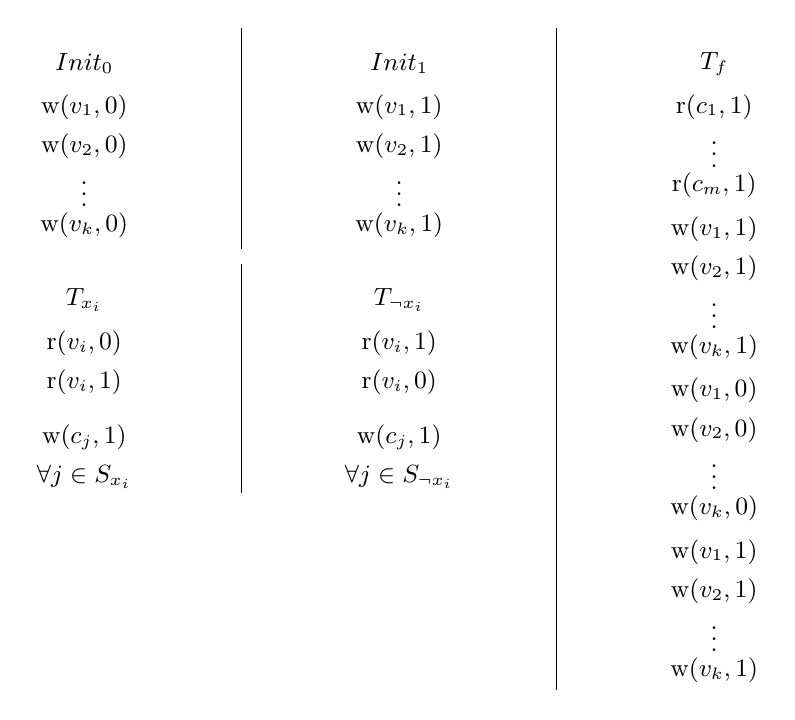
\begin{tikzpicture}[
    every node/.style={font=\small}
]

% =========================================================
% Init_0
% =========================================================

\node at (0,0) {$Init_0$};

\node at (0,-0.55) {$\mathrm{w}(v_1,0)$};
\node at (0,-1.05) {$\mathrm{w}(v_2,0)$};
\node at (0,-1.55) {$\vdots$};
\node at (0,-2.05) {$\mathrm{w}(v_k,0)$};


% =========================================================
% Init_1
% =========================================================

\node at (4.0,0) {$Init_1$};

\node at (4.0,-0.55) {$\mathrm{w}(v_1,1)$};
\node at (4.0,-1.05) {$\mathrm{w}(v_2,1)$};
\node at (4.0,-1.55) {$\vdots$};
\node at (4.0,-2.05) {$\mathrm{w}(v_k,1)$};


% =========================================================
% T_{x_i} -- below Init_0
% =========================================================

\node at (0,-3.0) {$T_{x_i}$};

\node at (0,-3.55) {$\mathrm{r}(v_i,0)$};
\node at (0,-4.05) {$\mathrm{r}(v_i,1)$};

\node at (0,-4.75) {$\mathrm{w}(c_j,1)$};
\node at (0,-5.25) {$\forall j\in S_{x_i}$};


% =========================================================
% T_{\neg x_i} -- below Init_1
% =========================================================

\node at (4.0,-3.0) {$T_{\neg x_i}$};

\node at (4.0,-3.55) {$\mathrm{r}(v_i,1)$};
\node at (4.0,-4.05) {$\mathrm{r}(v_i,0)$};

\node at (4.0,-4.75) {$\mathrm{w}(c_j,1)$};
\node at (4.0,-5.25) {$\forall j\in S_{\neg x_i}$};


% =========================================================
% T_f
% =========================================================

\node at (8.0,0) {$T_f$};

\node at (8.0,-0.55) {$\mathrm{r}(c_1,1)$};
\node at (8.0,-1.05) {$\vdots$};
\node at (8.0,-1.55) {$\mathrm{r}(c_m,1)$};

\node at (8.0,-2.10) {$\mathrm{w}(v_1,1)$};
\node at (8.0,-2.60) {$\mathrm{w}(v_2,1)$};
\node at (8.0,-3.10) {$\vdots$};
\node at (8.0,-3.60) {$\mathrm{w}(v_k,1)$};

\node at (8.0,-4.15) {$\mathrm{w}(v_1,0)$};
\node at (8.0,-4.65) {$\mathrm{w}(v_2,0)$};
\node at (8.0,-5.15) {$\vdots$};
\node at (8.0,-5.65) {$\mathrm{w}(v_k,0)$};

\node at (8.0,-6.20) {$\mathrm{w}(v_1,1)$};
\node at (8.0,-6.70) {$\mathrm{w}(v_2,1)$};
\node at (8.0,-7.20) {$\vdots$};
\node at (8.0,-7.70) {$\mathrm{w}(v_k,1)$};


% =========================================================
% Vertical separators
% =========================================================

\draw (2.0,0.45) -- (2.0,-2.35);
\draw (2.0,-2.55) -- (2.0,-5.45);
\draw (6.0,0.45) -- (6.0,-7.95);

\end{tikzpicture}
\caption{Threads in the reduction for $\rlxmm$}
    \label{tab:reduction-threads-relaxed}
\end{figure}

The threads $\mathsf{Init}{1}$ and $\mathsf{Init}{0}$ initialize the valuation used to evaluate the formula. For each variable $x_i$ corresponding to the Boolean variables of $\varphi$, $\mathsf{Init}{1}$ writes $1$ and $\mathsf{Init}{0}$ writes $0$. 
$T_{x_i}$ has a read statement $\rd(v_i,0)$ followed by $\rd(v_i,1)$ (which denotes reading \emph{true} for $x_i$) and sets all clauses containing $x_i$ to true, using the statement $\wt(c_j, 1)$ for all $j \in S_{x_i}$. 


Similarly, thread $T_{\neg x_i}$ reads $\rd(v_i, 1)$ followed by $\rd(v_i, 0)$ (denoting the value \emph{false} for $x_i$) and sets all clauses containing $\neg x_i$ to true. 
Finally the thread $T_{f}$ needs to make sure that all clauses are set to true, accomplished by the read statements $\rd(c_1, 1), \dots, \rd(c_m, 1)$.
Then, $T_{f}$ proceeds through the following steps (1) all the variables $v_i$s are set to $0$, followed by (2) setting all the variables $v_i$s to $1$, and finally (3) setting all the variables $v_i$s to $0$ again.
This sequence ensures that any threads $T_{x_i}$, $T_{\neg x_i}$ which were not executed in Phase 2 now have their conditions satisfied and can complete their execution. 
%%%%%%%%%

\begin{table}[h]
    
\noindent
\begin{minipage}{0.45\textwidth}
\centering
\begin{tabular}{c | c}
    $Init_0$ & $Init_1$ \\
    $\wt(v_1,0)$~& ~$\wt(v_1,1)$ \\ 
    $\wt(v_2,0)$~& ~$\wt(v_2,1)$ \\ 
    $\wt(v_3,0)$~& ~$\wt(v_3,1)$ \\

\end{tabular}
\vspace{.1cm}

\begin{tabular}{c | c}
    $T_{x_1}$ & $T_{\neg x_1}$ \\
    $\rd(v_1,0)$~& ~$\rd(v_1,1)$ \\ 
    $\rd(v_1,1)$~& ~$\rd(v_1,0)$ \\ 
    $\wt(c_1, 1)$~& ~ \\
    $\wt(c_2,1)$~&~ \\
\end{tabular}
\vspace{.1cm}

\begin{tabular}{c | c}
    $T_{x_2}$ & $T_{\neg x_2}$\\
     $\rd(v_2,0)$~& ~$\rd(v_2,1)$ \\ 
    $\rd(v_2,1)$~& ~$\rd(v_2,0)$ \\ 
    $\wt(c_2, 1)$~& ~ $\wt(c_2,1)$\\
\end{tabular}
\vspace{.1cm}

\begin{tabular}{c | c}
    $T_{x_3}$ & $T_{\neg x_3}$\\
     $\rd(v_3,0)$~& ~$\rd(v_3,1)$ \\ 
    $\rd(v_3,1)$~& ~$\rd(v_3,0)$ \\ 
    $\wt(c_2, 1)$~& ~ $\wt(c_2,1)$\\
   
\end{tabular}

\end{minipage}
\hfill
\begin{minipage}{0.45\textwidth}
\centering
\begin{tabular}{c}
    $T_f$ \\
     $\rd(c_1, 1)$ \\
    $\rd(c_2, 1)$ \\
    $\wt(v_1, 1)$ \\
    $\wt(v_2, 1)$ \\
    $\wt(v_3, 1)$ \\
    $\wt(v_1, 0)$ \\
    $\wt(v_2, 0)$ \\
    $\wt(v_3, 0)$ \\
    $\wt(v_1, 1)$ \\
    $\wt(v_2, 1)$ \\
    $\wt(v_3, 1)$ \\

\end{tabular}
\end{minipage}
\vspace{2em}
\caption{$\varphi=(x_1\lor x_2\lor x_3)\land (x_1 \lor \neg x_2\lor \neg x_3)$}
    \label{tab:relaxed-example-finegrainedwra}
\end{table}
%%%%%%%%%%%%%%%%

\begin{lemma}
    $\varphi$ is satisfiable iff $\expartial_\varphi  \models \rlxmm$.
\end{lemma}

\begin{proof}
    Suppose $A$ is a satisfying assignment for $\varphi$. We explictly describe the $\rf$ relation and $\mo$ relation as follows. 
    
    If $A(x_i) = true$:
    \begin{itemize}[leftmargin=0.1em]
    \item $\tuple{Init_0: \wt(v_i, 0)}~\rf~\tuple{T_{x_i}: \rd(v_i, 0)}$ and $\tuple{Init_1: \wt(v_i, 1)}~\rf~\tuple{T_{x_i}: \rd(v_i, 1)}$,
    \item $\tuple{T_f: \wt(v_i, 1)}~\rf~\tuple{T_{\neg x_i}: \rd(v_i, 1)}$, and $\tuple{T_f: \wt(v_i, 0)}~\rf~\tuple{T_{\neg x_i}: \rd(v_i, 0)}$. 
    \end{itemize} 
    Else, when $A(x_i) = false$, 
    \begin{itemize}[leftmargin=0.1em]
    \item $\tuple{Init_1: \wt(v_i, 1)}~\rf~\tuple{T_{\neg x_i}: \rd(v_i, 1)}$, and $\tuple{Init_0: \wt(v_i, 0)}~\rf~\tuple{T_{\neg x_i}: \rd(v_i, 0)}$,
    \item $\tuple{T_f: \wt(v_i, 0)}~\rf~\tuple{T_{ x_i}: \rd(v_i, 0)}$, and $\tuple{T_f: \wt(v_i, 1)}~\rf~\tuple{T_{ x_i}: \rd(v_i, 1)}$. 
    \end{itemize} 
            
    Coming to variables $c_i$s, for each $T_f: \rd(c_j, 1)$ there is a literal $\ell_j$ in clause $C_j$ that is true. Let $\tuple{T_{\ell_j}: \wt(c_j, 1)}~\rf~ \tuple{T_f: \rd(c_j, 1)}$. Observe that the constructed $\rf$ satisfies $\po-\rf$-acyclicity.
    
    The $\rf$ induces the following $\mo$ relation. If $A(x_i) = true$: 
    \begin{itemize}[leftmargin=0.1em]
    \item $\tuple{Init_0: \wt(v_i, 0)} ~\mo~\tuple{Init_1: \wt(v_i, 1)} ~\mo~\tuple{T_f: \wt(v_i, 1)}~\mo~\tuple{T_f: \wt(v_i, 0)} ~\mo~\\ \tuple{T_f: \wt(v_i, 1)}$
    \item For each clause $C_j$ there are three threads writing $\wt(c_j, 1)$.  For $C_j$, choose a specific literal $\ell_j$ that is made true by the satisfying assignment $A$. 
    The $\mo$ relation orders the write statements $\wt(c_j, 1)$ in literals that are set to true before $T_{\ell_j}: \wt(c_j, 1)$, and those in literals that set to false after $T_{\ell_j}: \wt(c_j, 1)$.
    \end{itemize}  
    When $A(x_i) = false$, an $\mo$ order can be defined analogously. 
    
    \begin{figure*}% 
\begin{center}
 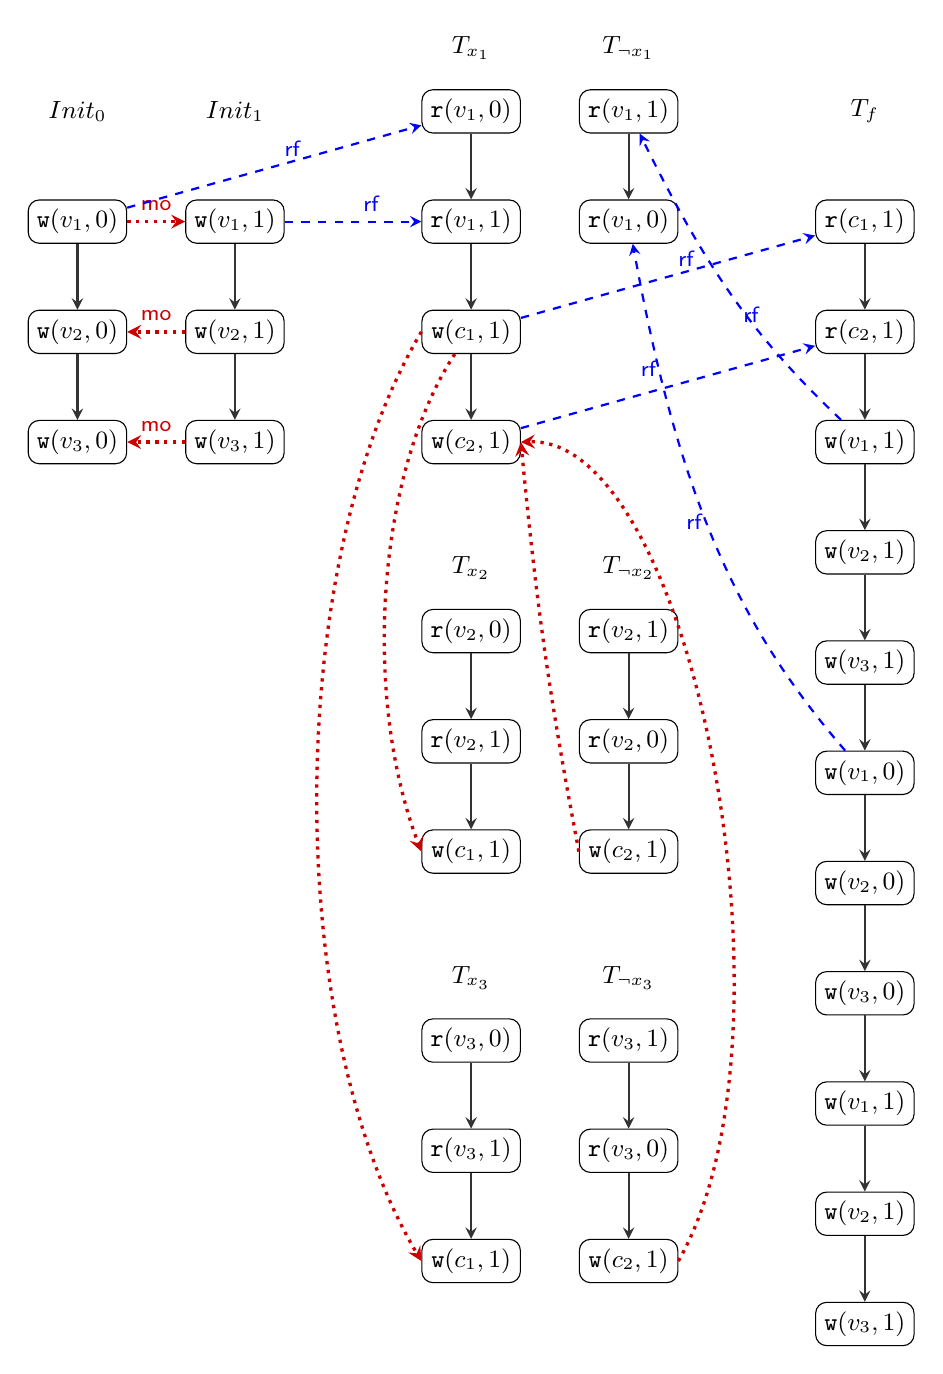
\begin{tikzpicture}[scale =1,yscale=2, 
    op/.style={draw, fill=white, rounded corners, minimum width=1.25cm, minimum height=0.55cm, 
               inner sep=2pt, font=\small},
    thread/.style={font=\small\bfseries},
    >=stealth
]

% ------------------------------------------------------------
% First group: T_i^1 and T_i^0
% ------------------------------------------------------------

% Init_0 / Init_1
\node[thread] (T11) at (0, 0.9) {$Init_0$};
\node[thread] (T10) at (2.0, 0.9) {$Init_1$};

\node[op] (i01) at (0, 0.2) {$\wt(v_1,0)$};
\node[op] (i02) at (0,-0.5) {$\wt(v_2,0)$};
\node[op] (i03)  at (0,-1.2) {$\wt(v_3,0)$};

\draw[po] (i01) to (i02);
\draw[po] (i02) to (i03);



\node[op] (i11) at (2.0, 0.2) {$\wt(v_1,1)$};
\node[op] (i12) at (2.0,-0.5) {$\wt(v_2,1)$};
\node[op] (i13)  at (2.0,-1.2) {$\wt(v_3,1)$};


\draw[po] (i11) to (i12);
\draw[po] (i12) to (i13);

\draw[mo] (i01) to node[above] {\footnotesize$\mo$} (i11);
\draw[mo] (i12) to node[above] {\footnotesize$\mo$} (i02);
\draw[mo] (i13) to node[above] {\footnotesize$\mo$} (i03);

% T_2^1 / T_2^0

% ------------------------------------------------------------
% Second group: T_xi and T_not xi
% ------------------------------------------------------------

% T_x1 / T_not x1
\node[thread] (Tx1)  at (5.0, 1.3) {$T_{x_1}$};
\node[thread] (Tnx1) at (7.0, 1.3) {$T_{\neg x_1}$};

\node[op] (v10) at (5.0,0.9) {$\rd(v_1,0)$};
\node[op] (v11) at (5.0,0.2) {$\rd(v_1,1)$};

\node[op] (c11)  at (5.0,-0.5) {$\wt(c_1,1)$};
\node[op] (c21)  at (5.0,-1.2) {$\wt(c_2,1)$};

\draw[po] (v10) to (v11);
\draw[po] (v11) to (c11);
\draw[po] (c11) to (c21);
\draw[rf] (i01) to node[above right] {\footnotesize$\rf$} (v10);
\draw[rf] (i11) to node[above right] {\footnotesize$\rf$} (v11);

\node[op] (v'11) at (7.0,0.9) {$\rd(v_1,1)$};
\node[op] (v'10) at (7.0,0.2) {$\rd(v_1,0)$};
\draw[po] (v'11) to (v'10); 

% T_x2 / T_not x2
\node[thread] (Tx2)  at (5.0,-2) {$T_{x_2}$};
\node[thread] (Tnx2) at (7.0,-2) {$T_{\neg x_2}$};

\node[op] (v20) at (5.0,-2.4) {$\rd(v_2,0)$};
\node[op] (v21) at (5.0,-3.1) {$\rd(v_2,1)$};
\node[op] (c12)  at (5.0,-3.8) {$\wt(c_1,1)$};

\draw[po] (v20) to (v21);
\draw[po] (v21) to (c12);

\node[op] (v'21) at (7.0,-2.4) {$\rd(v_2,1)$};
\node[op] (v'20) at (7.0,-3.1) {$\rd(v_2,0)$};
\node[op] (c22)  at (7.0,-3.8) {$\wt(c_2,1)$};

\draw[po] (v'21) to (v'20);
\draw[po] (v'20) to (c22);

% T_x3 / T_not x3
\node[thread] (Tx3)  at (5.0,-4.6) {$T_{x_3}$};
\node[thread] (Tnx3) at (7.0,-4.6) {$T_{\neg x_3}$};

\node[op] (v30) at (5.0,-5) {$\rd(v_3,0)$};
\node[op] (v31) at (5.0,-5.7) {$\rd(v_3,1)$};
\node[op] (c13)  at (5.0,-6.4) {$\wt(c_1,1)$};
\draw[po] (v30) to (v31);
\draw[po] (v31) to (c13);

\node[op] (v'31) at (7.0,-5) {$\rd(v_3,1)$};
\node[op] (v'30) at (7.0,-5.7) {$\rd(v_3,0)$};
\node[op] (c23)  at (7.0,-6.4) {$\wt(c_2,1)$};
\draw[po] (v'31) to (v'30);
\draw[po] (v'30) to (c23);

\draw[mo, bend right=45] (c11) to (c12.west);
\draw[mo, bend left=5] (c22.west) to (c21.east);
\draw[mo, bend right=50] (c11.west) to (c13.west);
\draw[mo, bend right=70] (c23.east) to (c21.east);

% ------------------------------------------------------------
% Final thread T_f
% ------------------------------------------------------------

\node[thread] (Tf) at (10.0,0.9) {$T_f$};

\node[op] (fc1) at (10.0,0.2) {$\rd(c_1,1)$};
\node[op] (fc2) at (10.0,-0.5) {$\rd(c_2,1)$};
\node[op] (fv11) at (10.0,-1.2) {$\wt(v_1,1)$};
\node[op] (fv21) at (10.0,-1.9) {$\wt(v_2,1)$};
\node[op] (fv31) at (10.0,-2.6) {$\wt(v_3,1)$};
\node[op] (fv10) at (10.0,-3.3) {$\wt(v_1,0)$};
\node[op] (fv20) at (10.0,-4.0) {$\wt(v_2,0)$};
\node[op] (fv30) at (10.0,-4.7) {$\wt(v_3,0)$};
\node[op] (fv'11) at (10.0,-5.4) {$\wt(v_1,1)$};
\node[op] (fv'21) at (10.0,-6.1) {$\wt(v_2,1)$};
\node[op] (fv'31) at (10.0,-6.8) {$\wt(v_3,1)$};

%po for Tf
\draw[po] (fc1) to (fc2);
\draw[po] (fc2) to (fv11);
\draw[po] (fv11) to (fv21);
\draw[po] (fv21) to (fv31);
\draw[po] (fv31) to (fv10);
\draw[po] (fv10) to (fv20);
\draw[po] (fv20) to (fv30);
\draw[po] (fv30) to (fv'11);
\draw[po] (fv'11) to (fv'21);
\draw[po] (fv'21) to (fv'31);

%rf edges

\draw[rf] (c11) to node[above right] {\footnotesize$\rf$} (fc1);
\draw[rf] (c21) to node[above left] {\footnotesize$\rf$} (fc2);
\draw[rf, bend left=10] (fv11) to node[below right] {\footnotesize$\rf$} (v'11);
\draw[rf, bend left=20] (fv10) to node[above left] {\footnotesize$\rf$} (v'10);


%\draw[rf, bend right=8] (s11b) to (fs12);
%\draw[rf, bend right=25] (s10a) to (fs11);
%\draw[rf, bend left=10] (s20b) to (fs22);
%\draw[rf, bend left=10] (s21a) to (fs21);
%\draw[rf, bend left=0] (s30b) to (fs32);
%\draw[rf, bend left=0] (s31a) to (fs31);
\end{tikzpicture}%
\end{center}
\caption{Execution graph for Table~\ref{tab:relaxed-example-finegrainedwra}: The graph is restricted to the $\mo$-edges between writes of $Init_1$ and $Init_0$ and all synthesized  edges involving $v_1$}
\label{example-Execution-relaxed}
\end{figure*}%

    
    Table~\ref{tab:relaxed-example-finegrainedwra} gives an instance of the construction of $\expartial$ for the fine-grained hardness reduction for \threewriter~ and (Figure~\ref{example-Execution-relaxed}) shows the synthesis of $\rf$ and $\mo$-edges. To keep the figure simple, and less confusing we have only showed the synthesized edges related to $v_1$. The execution graph is constructed for $x_1=1, x_2=0, x_3=0$, a satisfying assignment for $\varphi$. The $\rf$ and $\mo$-edges follow the rules of construction we just discussed. 
    
    

    \paragraph*{Relaxed Write-coherence.} From our construction, it is easy to see $\irr(\mo_x; \po)$.

    \paragraph*{Relaxed Read-coherence.} We need to prove  $\irr(\rf^{-1}; \mo_x; \rf^{?}; \po)$. 
    If relaxed read coherence is violated, the violating pattern is of the following form there are read events $r_1$ and $r_2$, and two write events $w_1, w_2$ such that $w_1~\rf~r_1$, $w_2~\rf~r_2$, $w_1~\mo~w_2$ and $r_2~\po~r_1$.
    Such a violation can potentially happen on variables which have multiple read events in the same thread, which is only the case for $v_i$.
    We consider the various possibilities below. 
    We consider the case $A(x_i) = true$ below. 
        \begin{itemize}[leftmargin=0.1em]
            \item $\tuple{T_{x_i}: \rd(v_i, 0)} \po \tuple{T_{x_i}: \rd(v_i, 1)}$, reads-from $Init_0$ and $Init_1$ respectively, where $\mo$ agrees with the $\po$.
            \item $\tuple{T_{\neg x_i}: \rd(v_i, 1)} \po \tuple{T_{\neg x_i}: \rd(v_i, 0)}$, reads-from the first two writes on $v_i$ in $T_f$ respectively, where, once again $\mo$ agrees with the $\po$, and irreflexivity is ensured.
        \end{itemize}
        A similar argument can be made for the case the case $A(x_i) = false$.

    This shows that the constructed $\rf$ and $\mo$ are consistent with $\rlxmm$. 
    
    
    
    Conversely, suppose $\expartial_\varphi \models \rlxmm$. 
    We need to show that there are no two $\rd(c_j, 1)$ and $\rd(c_\ell, 1)$ reading from some $T_{x_i}$ and $T_{\neg x_i}$.
    Suppose not. 
    Let $\rd(c_j, 1)$ read from $T_{x_i}: \wt(c_j, 1)$ and $\rd(c_\ell, 1)$ read from $T_{\neg x_i}: \wt(c_\ell, 1)$.    
    Consider the thread $T_{x_i}$. Since $T_{x_i}: \wt(c_j, 1)$ has been read from, this means that the preceding read instructions of $T_{x_i}$ have been executed, and the only possible read from relation is as follows: 
    $\tuple{Init_0: \wt(v_i, 0)}~\rf~\tuple{T_{x_i}: \rd(v_i, 0)}$,
    and $\tuple{Init_1: \wt(v_i, 1)}~\rf~\tuple{T_{x_i}: \rd(v_i, 1)}$. 
    By relaxed read coherence axiom, this implies $\tuple{Init_0: \wt(v_i, 0)} ~\mo~\tuple{Init_1: \wt(v_i, 1)}$    

    Now, consider the thread $T_{\neg x_i}$. As argued fro $T_{x_i}$, since the last instruction has been read from, the preceding read instructions of $T_{x_i}$ have been executed with the only reads-from relation being 
    $\tuple{Init_1: \wt(v_i, 1)}~\rf~\tuple{T_{\neg x_i}: \rd(v_i, 1)}$ and $\tuple{Init_0: \wt(v_i, 0)}~\rf~\tuple{T_{\neg x_i}: \rd(v_i, 0)}$. 
    However, this violates relaxed read coherence axiom, as $\tuple{Init_0: \wt(v_i, 0)} ~\mo~\tuple{Init_1: \wt(v_i, 1)}$ but $\tuple{T_{\neg x_i}: \rd(v_i, 1)}~\po~\\ \tuple{T_{\neg x_i}: \rd(v_i, 0)}$. 
    This contradicts our assumption that there are two $\rd(c_j, 1)$ and $\rd(c_\ell, 1)$ reading from some $T_{x_i}$ and $T_{\neg x_i}$. 
    Thus, the assignment induced by the $T_i^b$ threads executed before $T_f$ satisfies $\varphi$.
\end{proof}

The above lemma prove Theorem~\ref{lem:relaxed-finegrained}.

In the next section we show that the $\vm$ problem is NP-hard for $\twowriter$. 

\section{NP-hardness for \twowriter\ systems}
\label{sec:np-relaxed}
Given a 3-CNF-SAT formula $\varphi$ with $k$ variables and $m$ clauses, we construct an abstract execution $\ypartial=(\E, \po)$ with $2k+m+3$ threads, accessing $k+2m+1$ memory locations $v_1, v_2, \dots, v_k, c_1, \dots, c_m, d_1, \dots, d_m, s$ and 2 values $0, 1$ such that $\varphi$ is satisfiable iff $\ypartial_\varphi^{\rlxmm}  \models \rlxmm$.
$\ypartial_\varphi^{\rlxmm}$ follows the general scheme depicted in Figure~\ref{fig:two-writer} of Chapter~\ref{RA-ptime}.

As in Section~\ref{sec:hardness-twowriter}, here also we face similar challenge of reducing the number of writers for $c_j$ to two. But besides this, we also need to reduce the number of writers for $v_i$'s. The former challenge is handled the same way as the $\twowriter$ construction in Section~\ref{sec:hardness-twowriter}. For the later challenge we do the following.
\begin{itemize}
 \item Remove all the writes from $T_f$ in $\expartial_{\varphi}$, and add it to $Init_1$ after $\wt(v_k,1)$. The order of the writes remain same as before.
 
\item So that the above writes can be executed only after $T_f$, add a $\wt(s,1)$ after the last read i $T_f$ and a $\rd(s,1)$ before newly the added  set of writes in $Init_1$.
\end{itemize}

The required changes to Table~\ref{tab:reduction-threads-relaxed} is reflected in Table~\ref{tab:np-reduction-threads-relaxed}

In this reduction also, a formula $\varphi$ with $k$ threads and $m$ clauses yields an execution graph with $\mathcal{O}(k + m)$ theads and this does not give the stronger hardness under ETH, parameterized by the number of threads. 

\begin{theorem}
\label{thm:relaxed-two-writer-hardness}
    The $\vm$ problem is $\NP$-complete for $\rlxmm$, even when restricted to \twowriter\ execution graphs.
\end{theorem}

The above theorem can be proved by the next two lemmas.

\begin{table}[h]
    
\noindent
\begin{minipage}{0.17\textwidth}
\centering
\begin{tabular}{c | c}
    $Init_0$ & $Init_1$ \\
    $\wt(v_1, 0)$~& ~$\wt(v_1, 1)$ \\
    $\wt(v_2, 0)$~ & ~$\wt(v_2, 1)$ \\
    $\cdots$ \\
    $\wt(v_k, 0)$~ & ~$\wt(v_k, 1)$\\
    & $\rd(s, 1)$ \\
    & $\wt(v_1, 0)$ \\
    & $\wt(v_2, 0)$ \\
    & $\cdots$ \\
    & $\wt(v_k, 0)$ \\
    & $\wt(v_1, 1)$ \\
    & $\wt(v_2, 1)$ \\
    & $\cdots$ \\
    & $\wt(v_k, 1)$ \\
    
\end{tabular}
\end{minipage}
\hfill
\begin{minipage}{0.35\textwidth}
\centering
\begin{tabular}{c | c}
    $T_{x_i}$~ & ~$T_{\neg x_i}$ \\
        $\rd(v_i, 0)$ ~&~  $\rd(v_i, 1)$ \\
        $\rd(v_i, 1)$ ~&~ $\rd(v_i, 0)$ \\
        & \\        
        $\wt(c_j, 1)$ ~&~ $\wt(c_j, 1)$ \\
        $\forall j \in S_{x_i}\setminus S_{x_i}^{3}$ ~&~  $\forall j \in S_{\neg x_i}\setminus S_{\neg x_i}^{3}$\\
        $\wt(d_j,1)$, $j\in S_{x_i}^{3}$~&~ $\wt(d_j,1)$, $j\in S_{\neg x_i}^{3}$\\
        \scriptsize $S_{x_i}^{3}=\{j:\ell_j^3=x_i\}$ ~&~  \scriptsize $S_{\neg x_i}^{3}=\{j:\ell_j^3=\neg x_i\}$
        
\end{tabular}
\end{minipage}
\hfill
\begin{minipage}{0.13\textwidth}
\centering
\begin{tabular}{c}
    $T_j$ \\
    $\rd(c_j, 1)$\\
    $\wt(d_j, 1)$ \\
    $\forall j \in \{1,\cdots,m\}$\\
\end{tabular}
\end{minipage}
\hfill
\begin{minipage}{0.13\textwidth}
\centering
\begin{tabular}{c}
    $T_f$ \\
    $\rd(d_1, 1)$ \\
    $\rd(d_2, 1)$ \\
    $\cdots$ \\
    $\rd(d_m, 1)$ \\
    $\wt(s, 1)$ \\
\end{tabular}
\end{minipage}
\vspace{2em}
\caption{Threads in the reduction for $\rlxmm$}
    \label{tab:np-reduction-threads-relaxed}
 %\vspace{-.8cm}   
\end{table}

\begin{lemma}
    $\varphi$ is satisfiable iff $\ypartial_\varphi^{\rlxmm}  \models \rlxmm$.
\end{lemma}

\begin{proof}
    Suppose $A$ is a satisfying assignment for $\varphi$. Then, the execution proceeds as follows. 
    The $\rf$ relation and $\mo$ relation are exactly as in Lemma~\ref{lem:relaxed-finegrained}, except the following.
    If $A(x_i) = true$:
    \begin{itemize}
        \item $\tuple{T_f: \wt(s, 1)}~\rf~\tuple{Init_1: \rd(s, 1)}$,
        \item $\tuple{Init_1: \wt(v_i, 1)}~\rf~\tuple{T_{\neg x_i}: \rd(v_i, 1)}$, and $\tuple{Init_1: \wt(v_i, 0)}~\rf~\tuple{T_{\neg x_i}: \rd(v_i, 0)}$. 
    \end{itemize} 
    For clause variables $c_j$ and $d_j$ , the $\rf$ (and consequently $\mo$) relation depends on the literals set to true by $A$. 
    For each clause $C_j$ there are two threads writing $\wt(c_j, 1)$, and two threads writing $\wt(d_j, 1)$. 
    
    If $A$ makes $\ell_j^3$ true then $\tuple{T_{\ell_j^3}: \wt(d_j, 1)}~\rf~\tuple{T_f: \rd(d_j, 1)}$. Otherwise $A$ makes $\ell_j^1$ or $\ell_j^2$ true. Let $\ell_j^k$ be the literal that is made true by the satisfying assignment $A$. Then, we have $\tuple{T_{\ell_j^k}: \wt(c_j, 1)}~\rf~\tuple{T_j: \rd(c_j, 1)}$ and $\tuple{T_j: \wt(d_j, 1)}~\rf~\tuple{T_f: \rd(d_j, 1)}$.

%    If $A$ makes $\ell_j^1$ or $\ell_j^2$ true, then $\tuple{T_{\ell_j^3}: \wt(d_j, 1)}~\rf~\tuple{T_f: \rd(d_j, 1)}$. Otherwise, $\tuple{T_j: \wt(d_j, 1)}~\rf~\tuple{T_f: \rd(d_j, 1)}$.
    For every variable-value pair for $c_j$ and $d_j$, there are atmost two writes. With the $\rf$ picked as above, the $\mo$ relation gets fixed: the unused write in $T_{x}$/ $T_{\neg x}$ that is set to true by $A$ is $\mo$-before the used write, while if the unused write is in $T_{x}$/ $T_{\neg x}$ that is set to false by $A$, then it is $\mo$-after the used write.    
    
    \paragraph*{Relaxed Write-coherence.} From our construction, it is easy to see $\irr(\mo_x; \po)$.
    %, which is easy to see from our construction. 

    \paragraph*{Relaxed Read-coherence.} We need to prove  $\irr(\rf^{-1}; \mo_x; \rf^{?}; \po)$. 
    The possible violating patterns and the arguments follow as in Lemma~\ref{lem:relaxed-finegrained}.

    This yields an $\rf$ where all $\rd(d_j, 1)$ in $T_f$ read from a thread corresponding to a true literal in $A$, so $\ypartial_\varphi^{\rlxmm} \models \rlxmm$.

    
    
    Conversely, suppose $\ypartial_\varphi^{\rlxmm} \models \rlxmm$. 
    The proof proceeds as in Lemma~\ref{lem:relaxed-finegrained}, where we show that if there are two clauses $C_j$ and $C_{\ell}$ such that $\rd(d_j, 1)$ and $\rd(c_\ell, 1)$ reading from some $T_{x_i}$ and $T_{\neg x_i}$, then relaxed read coherence is violated. .
\end{proof}


\section{Discussion}
We thus give similar trichotomy of results for the $\vm$-problem, as in case of $\ramm$-variants, with poynomial time for \onewriter{}, NP-Completenes for \twowriter{} and a fine-grained lower bound assuming ETH for \threewriter{}.  Note that we do not provide any conditional lower bound for relaxed as we did for $\ramm$ and their variants in Section~\ref{sec:1-writer-hardness} of Chapter~\ref{RA-ptime}. There we had reduced detecting triangle in a graph to the problem of consistency testing for $\onewriter$ systems under $\wramm$.  
To extend the construction to  Relaxed, \RlxRCoh should be violated on detecting a triangle. Violating relaxed-read-coherence needs either (i) two writes $\wt_1$, $\wt_2$ to a variable in different threads such that $\wt_1\mo\w$, are read by $\po$-related reads $\rd_1,~ \rd_2$ such that the $\po$-later
read reads from the mo-earlier write, or (ii) two writes $\wt_1$, $\wt_2$ in the same thread to a variable which
are read by po-related reads $\rd_1$, $\rd_2$ in the opposite order. (i) cannot be done with single-writer, while
(ii) violates relaxed-read-coherence irrespective of a triangle detection. So, it is not clear if such a superlinear lower bound exists for $\rlxmm$ and we keep it open. In the next chapter we prove similar type of results for the Causal Memory Models. We also provide the necessary axioms and examples to show how these models are related to the release-acquire fragment of C11. 




 



%%%%%%%%%%%%%%
\newtheorem{definition}{Definition}
\chapter{Verifying Causal Memory Models}
 Closely related to these memory models are $\rlxmm$~ and causal consistency models~\cite{BouajjaniEGH17,Burckhardt:2014}
 
 \section{Causal Consistency Models}
\label{app:cc-models}


In this appendix, we study the consistency checking problem under the \emph{causal consistency models} namely, $\ccmm, \cmmm$ and $\cvmm$ which come from distributed databases.
We begin with a brief overview of the
operational and axiomatic semantics of these models, and then show that the complexity landscape observed for the Release - Acquire (RA) variants extends to these models as well. 
Recall that for RA, we established a tight characterization of complexity with respect to the number of writer threads per memory location:
\onewriter\ admits polynomial-time
solutions, \twowriter\ is $\NP$-hard, and \threewriter\ yields a stronger
conditional lower bound. Our goal in this section is to establish analogous
results for causal consistency models, thereby showing that the same complexity results extend to $\ccmm, \cmmm$ and $\cvmm$. Next, we provide an overview of these causal consistency models. 


\subsection{Overview of Causal Consistency Models}
\label{app:cc-models-overview}

In the domain of distributed systems, causality is the key concept for consistency. There are three popular causal models, namely, Causal Consistency ($\ccmm$), Causal Convergence ($\cvmm$), and Causal Memory ($\cmmm$)~\cite{BouajjaniEGH17}. 
It is known that $\ccmm$ coincides with $\wramm$ while $\cvmm$ coincides with $\sramm$~\cite{Lahav:2022}. $\cmmm$ is stronger than $\ccmm$ and incomparable to $\cvmm$ and $\ramm$.  

In Causal Memory, each thread has a locally-consistent view of the order that different writes have been executed~\cite{Ahamad1995,BouajjaniEGH17}. 
This is formalised by introducing an additional relation for each thread, called the ``happened-before'' relation in the literature.  To avoid confusion with the ``happens before'' $\hb$, we call this the \emph{observed relation} $\ob{}$. 

To enhance understanding we define the notion of \emph{conflicting triplets} first.

\begin{definition}(Conflicting Triplet)
Given an execution graph $\expartial=(\E,\po)$, two events in $\E$ are called \emph{conflicting} if both are on the same variable and at least one of them is a write. If also the reads-from function $\rf$ is given, a \emph{Conflicting Triplet} is defined as a tuple $(\wt, \rd, \wt')$ of pairwise conflicting events in $\E$ such that $\wt~\rf~\rd$. 
\end{definition} 
 
\noindent{The observed relation $\ob{}$.}
Given an event $\event$, the \emph{observed relation} for $\event$ is the smallest transitive relation $\ob{\event}\subseteq \E\times \E$ with the following properties. 

\begin{enumerate}
\item For every $(\event_1, \event_2)\in \hb$ such that $(\event_i, \event)\in \hb$ for each $i\in[2]$, we have $(\event_1, \event_2)\in \ob{\event}$.
\item For every conflicting triplets $(\wt, \rd, \wt')$ such that:
(ii)~$(\wt',\rd)\in \ob{\event}$ and
(iii)~$(\rd, \event)\in \po^?$,
we have $(\wt', \wt)\in \ob{\event}$.
\end{enumerate}


The idea is that any thread which executes the read $\rd$ must observe $\wt$ 
after it has observed $\wt'$ so that it does not read an obsolete value. 
For any event $\event$, $\ob{\event}$ contains $\hb$, and $\ob{}$ grows monotonically as we move down a thread 
in $\po$-order. That is, for any $(\event_1, \event_2)\in \po$, we have $\ob{\event_1}\subseteq \ob{\event_2}$. For a thread $t$, the observed relation  is defined as $\ob{t}=\ob{\event^{\max}}$, where $\event^{\max}$ is the $\po$-maximal event of $t$.  $\cmmm$ requires all the axioms of $\wramm$, and in addition, 
requires that $\ob{t}$ is irreflexive~\cite{BouajjaniEGH17}. Figure \ref{cm:examples} depicts 
some examples. 

\begin{itemize}
\item $(\text{PORF})\land(\text{weak-Rcoh})\land (\text{\OB{}})$ \hfill [$\cmmm$]
\end{itemize}

Thus, $\wramm\mmorder \cmmm$. However, $\cmmm$ is incomparable with $\ramm$/$\sramm$, i.e., $\cmmm$ allows executions that are inconsistent in $\ramm$/$\sramm$ and vice versa. 


	\begin{figure}
	\centering
	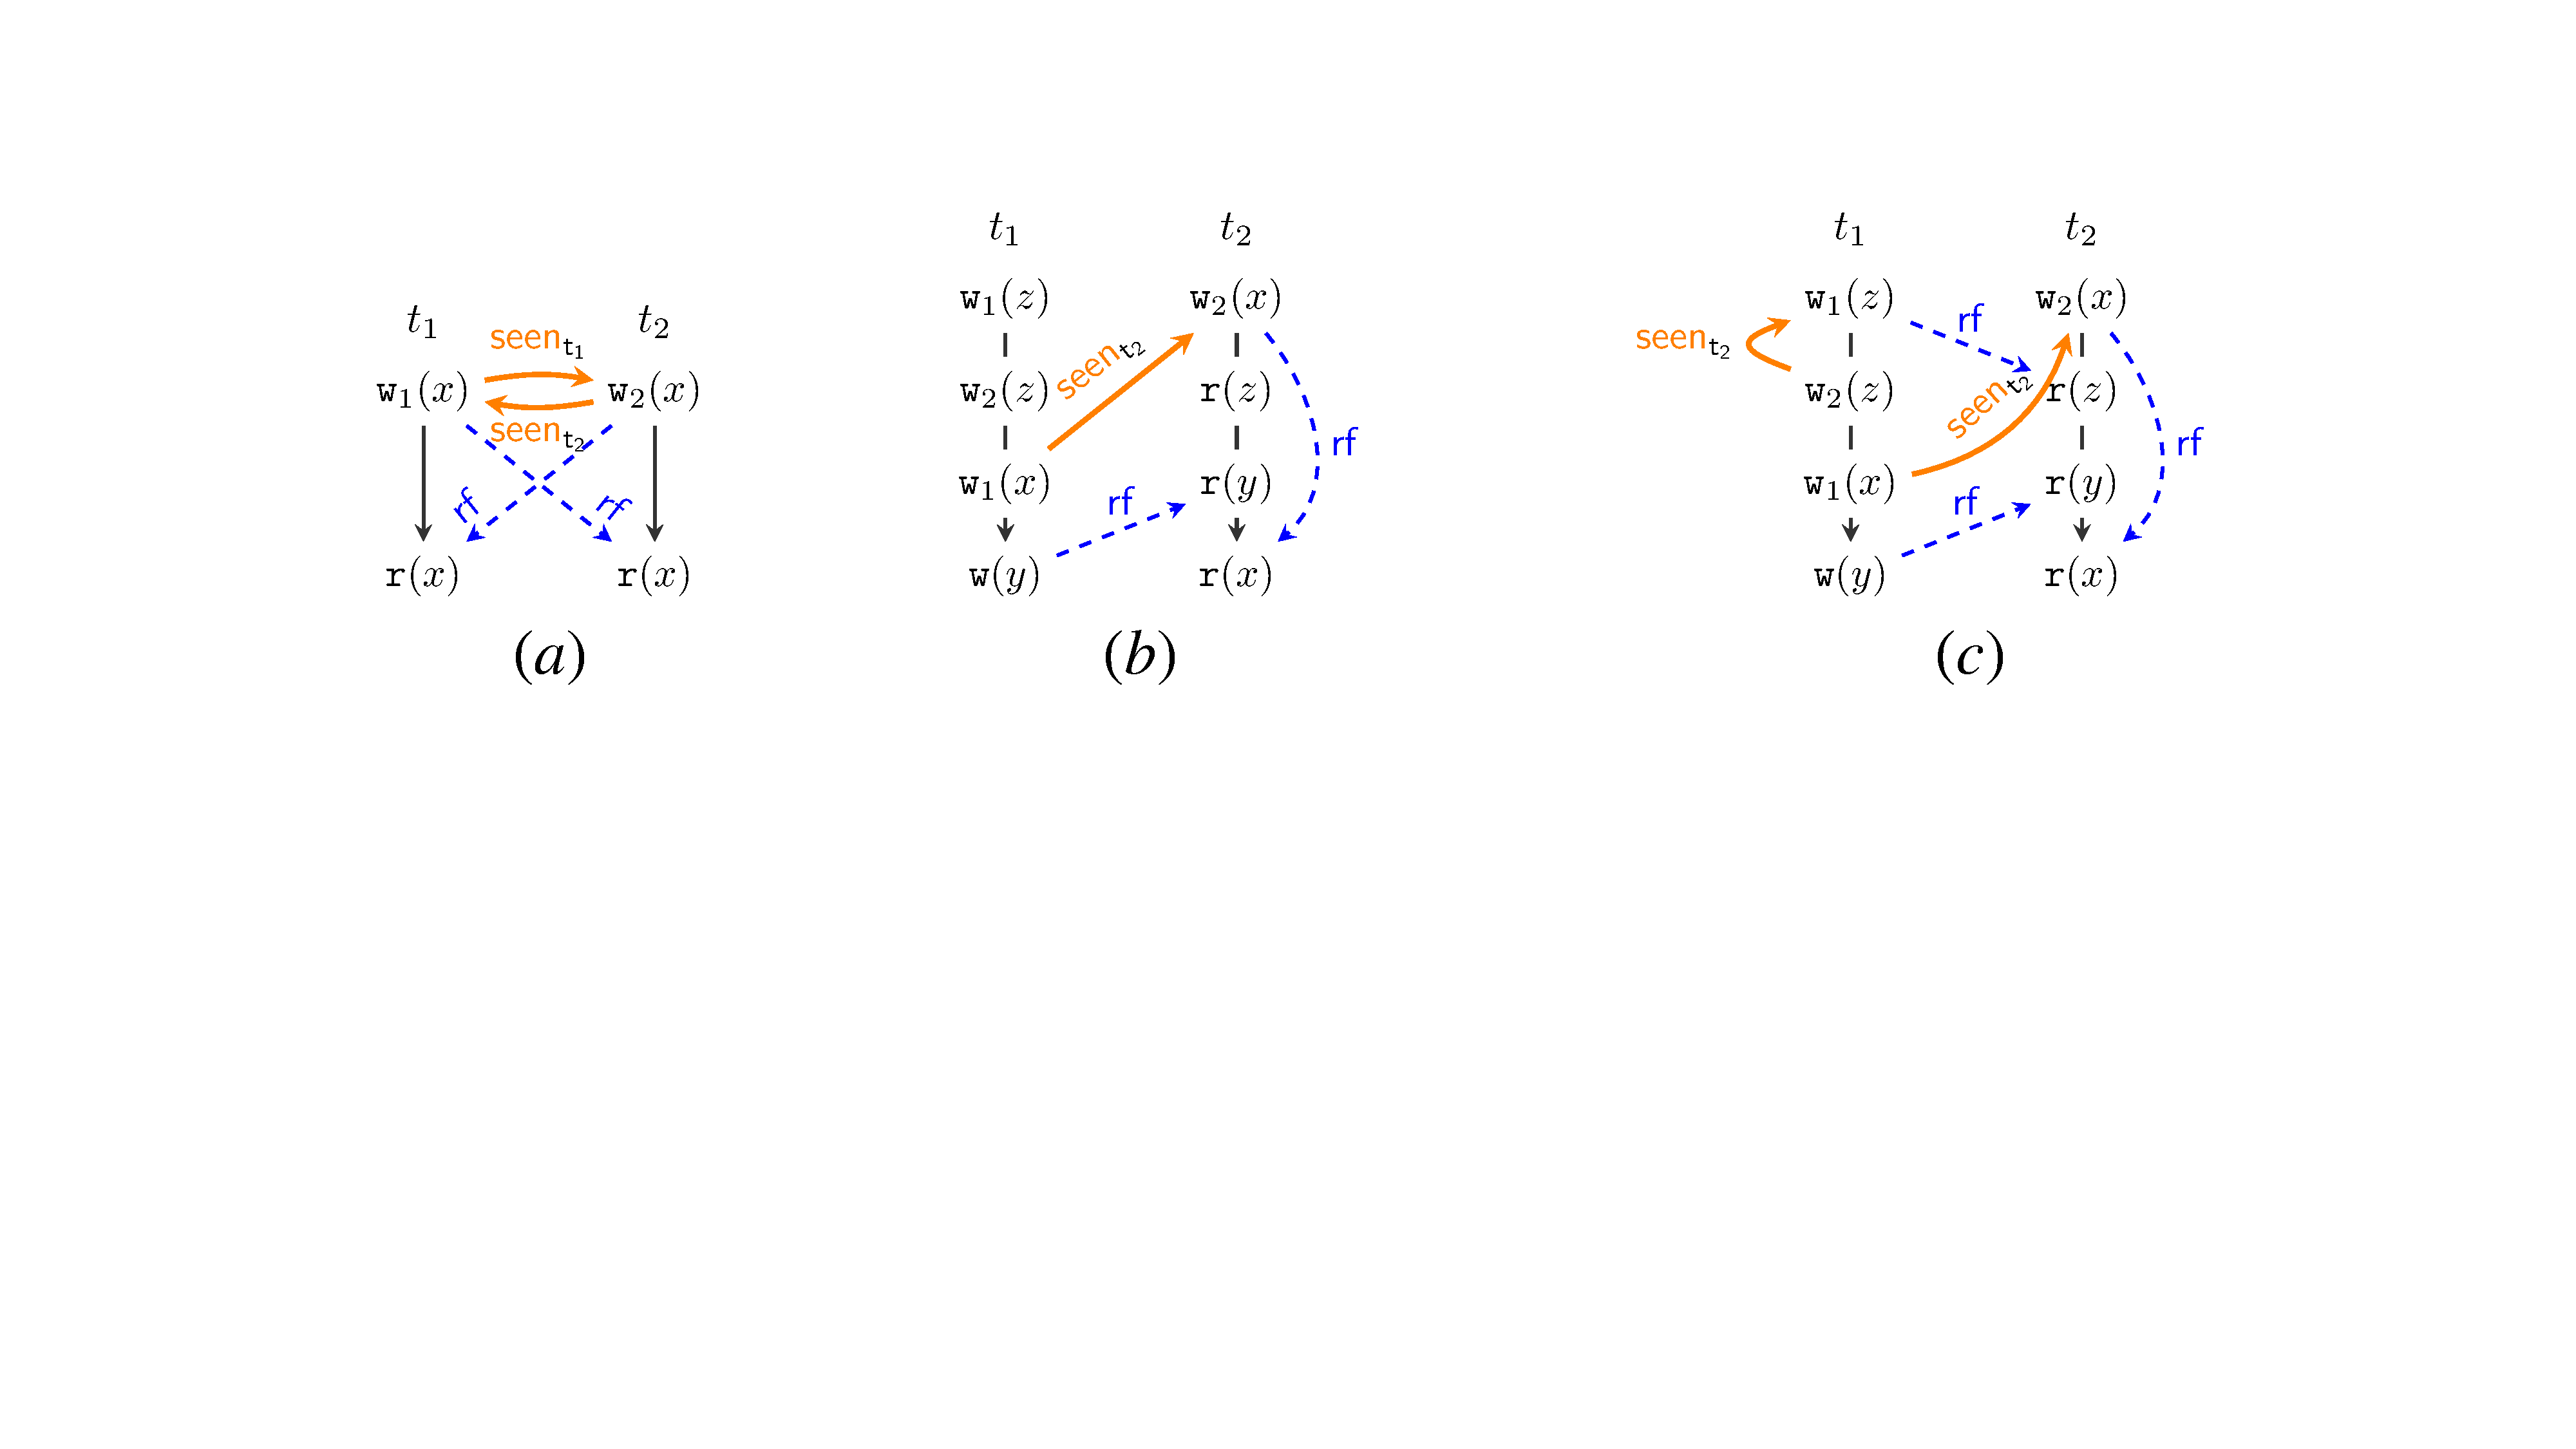
\includegraphics[width=\textwidth]{Figures/CM.pdf}
	\caption{(a) is $\cmmm$ consistent as $\ob{t_1}, \ob{t_2}$ are acyclic. 
	(b) is also $\cmmm$ consistent : the $\wt_1(x) \ob{t_2} \wt_2(x)$ is induced 
	by $\wt_1(x)~\hb~\rd(x)$ and $\wt_2(x)~\rf~\rd(x)$. 
	(c) is obtained 
	from (b) by adding $\wt_1(z)~\rf~\rd(z)$, and is $\cmmm$ inconsistent, 
since we have $\wt_1(z)~\po~\wt_2(z)~\ob{t_2}~\wt_1(z)$. 
	$\wt_2(z)~\ob{t_2}~\wt_1(z)$ is induced 
	from the conflicting triplet $(\wt_1(z), \rd(z), \wt_2(z))$ with 
	 $\wt_2(z)~\ob{t_2}~\rd(z)$. 
	}
	\label{cm:examples}
	\end{figure}

Since $\wramm=\ccmm$ and $\sramm=\cvmm$, both the fine-grained-hardness and $\NP$-hardness result for $\wramm, \sramm$ implies the same for  $\ccmm$ and $\cvmm$. So we only need to prove the hardness results for $\cmmm$.
In Section \ref{app:cc-1w}, we discuss the polynomial-time algorithm for \onewriter\ programs and in Section~\ref{app:cc-3w}, we discuss the complexity results for \threewriter\ programs under $\cmmm$. Note that the $\NP$-hardness for \twowriter\ programs under $\cmmm$ follows from arguments analogous to those made in Section~\ref{sec:hardness-twowriter} for RA models, and therefore we do not discuss it separately.

 	

For a $\cmmm$-consistent execution graph the following should be satisfied: $(\text{PORF})\land(\text{weak-Rcoh})\land (\text{\OB{}})$



 


\subsection{ \onewriter~ programs under Causal Consistency }~\label{app:cc-1w}

Recall that $\cmmm$ is essentially $\wramm$ with the extra axiom of $\ob{}$ acyclicity. We argue that the algorithm in  Section~\ref{sec:onewriter-algorithm} 
can be used for $\cmmm$ also. It is easy to see that any execution graph $\ex$  which is $\cmmm$-consistent is also $\wramm$-consistent. 


The other direction follows for the \onewriter{} case. 
Suppose $\ex$ is $\wramm$-consistent but  violates $\ob{t}$ acyclicity for some thread 
 $t$. Then we have  both $\wt'~\ob{t}~ \wt$ and  $\wt~\ob{t}~ \wt'$ for writes $\wt, \wt'$ on some location $x$. 
 
 By definition of $\ob{t}$, $\wt'~\ob{t}~ \wt$ implies the existence of a conflicting triplet $(\wt, \rd, \wt')$ such that 
   $\wt~\rf ~\rd$, $\wt'~\ob{t}~\rd$, $\rd~\po^?~ e_{max}$ where $e_{max}$ is the $\po$-maximal element of $t$.
  Likewise,  $\wt~\ob{t}~ \wt'$ implies the existence of a conflicting triplet $(\wt', \rd', \wt)$ such that 
   $\wt'~\rf ~\rd'$, $\wt~\ob{t}~\rd'$, $\rd'~\po^?~ e_{max}$ where $e_{max}$ is the $\po$-maximal element of $t$. 
      Since $\wt, \wt'$  are in the same thread, either $\wt~\po~\wt'$ or 
   $\wt'~\po~\wt$. Either way, we observe one violation for \WRCoh{} wrt $\rd$ or $\rd'$. 
   Thus, inconsistency wrt $\cmmm$ results in $\wramm$ inconsistency as well. 
    Therefore, the algorithm    for $\wramm$ can be employed for $\cmmm$ as well. 
   Thus in case of \onewriter~ the time complexity of consistency testing will be same as that of $\wramm$, $O(n^3)$. 
   
   Since $\cvmm = \sramm$ and $\ccmm=\wramm$, the lower bound result under BMM hypothesis in Section~\ref{sec:onewriter} holds for both $\cvmm$ and $\ccmm$. Finally, as mentioned previously,
for the single writer case, obtaining a cyclic $\ob{t}$ for a thread $t$ results in violation of \WRCoh{}.  In the reduction given in Section~\ref{sec:onewriter}, \WRCoh{} is violated in the presence of a triangle, hence, the result also holds for $\cmmm$.
   
   





\subsection{Fine-grained Hardness under ETH for \threewriter~ systems}~\label{app:cc-3w}


We will now discuss the fine-grained hardness of \threewriter -system under $\cmmm$. 
Since  $\cmmm$ is stronger than $\wramm$, the soundness part of the reduction in 
 Lemma \ref{lem:wra-eth}  follows : Assume $\expartial_\varphi^{\ramm} \models \cmmm$. Then 
 we know $\expartial_\varphi^{\ramm} \models \wramm$. Our soundness argument shows that 
 $\varphi$ is satisfiable. 
 
 For the completeness part, assume that $\varphi$ is satisfiable. We have already synthesized an $\rf, \mo$ which respect $\sramm$(and hence $\wramm$). We have to now show that, \OB{} is preserved by the synthesized $\rf$. 

\begin{lemma}\label{lem:eth-cm}
If $\varphi$ has a satisfying assignment, then $\expartial_\varphi^{\ramm} \models \cmmm$. 
\end{lemma}
\begin{proof}
Let $A$ be the satisfying assignment for $\varphi$. 
Say $A(x_i) = true$:

(i) For all pair of events in $\E$, $e~\hb~e'$ we have $e~\ob{T_F}~e'$

(ii) For the conflicting tiplet $(\tuple{T_i^0: \wt(s_i, 1)}, \tuple{T_f: \rd(s_i, 1)}, \tuple{T_i^1: \rd(s_i, 2)})$, we have $\tuple{T_i^1: \wt(s_i, 2)}~ \ob{T_f}~ \tuple{T_f: \rd(s_i, 1)}$ and $\tuple{T_f: \rd(s_i, 1)}~\po^?~e^{T_f}_{max}$ where $e^{T_f}_{max}$ is the $\po$-maximal event in $T_f$. This implies $\tuple{T_i^1: \wt(s_i, 2)}~\ob{T_f}~\tuple{T_i^0: \wt(s_i, 1)}$. 

As there are no $\hb$-cycle and no members of $\ob{T_f}$ directed from $T_i^0$ to $T_i^1$, $\ob{T_f}$ is irreflexive.

If we consider the relation $\ob{T_{\neg x_i}}$, for the conflicting triplet $(\tuple{T_i^0: \wt(v_i, 0)},\\ \tuple{T_{x_i}: \rd(v_i,0)}, \tuple{T_i^1: \wt(v_i, 1)})$ we have $\tuple{T_i^1: \wt(v_i, 1)}~\ob{T_{\neg x_i}}~\tuple{T_i^0: \wt(v_i, 0)}$. 

Again no members of $\ob{T_{\neg x_i}}$ are directed from $T_i^0$ to $T_i^1$. As there is no $\hb$-cycle, $\ob{T_{\neg x_i}}$ is also irreflexive. 

It is easy to see that $\ob{}$ is irreflexive for all remaining threads.
Hence \OB{} is preserved by the synthesized $\rf$

\end{proof}

\subsection{NP-hardness for \twowriter~ systems}

For \twowriter~ systems the reduction from 3-SAT instance has similar construction as that of $\wramm$ and the proof of the reduction will be on similar argument as the proof of the reduction for \threewriter.




 \chapter{Discussions and Future Work}

\bibliographystyle{IEEEtran}
\bibliography{m}

\end{document}
